\documentclass[twocolumn,9pt]{revtex4-2}

\usepackage{graphicx}
\usepackage{amsmath}
\usepackage{amssymb}
\usepackage{geometry}
\usepackage{natbib}
\usepackage{setspace}
\usepackage{bm}
\usepackage[hidelinks]{hyperref}
\usepackage[colorlinks=true,
            linkcolor=blue,
            citecolor=blue,
            urlcolor=blue]{hyperref}
\usepackage[nameinlink]{cleveref}

\geometry{margin=0.7in}
\setstretch{1.14}

\begin{document}

\title{
Earth-Fixed Geometric Structure, Bistable Dynamics, and Phase-Locked Planetary Torque Coupling in Polar Motion
}

\author{
Craig Stone
}

\date{1 May 2026}

\maketitle

\begin{figure*}[htbp]
\centering
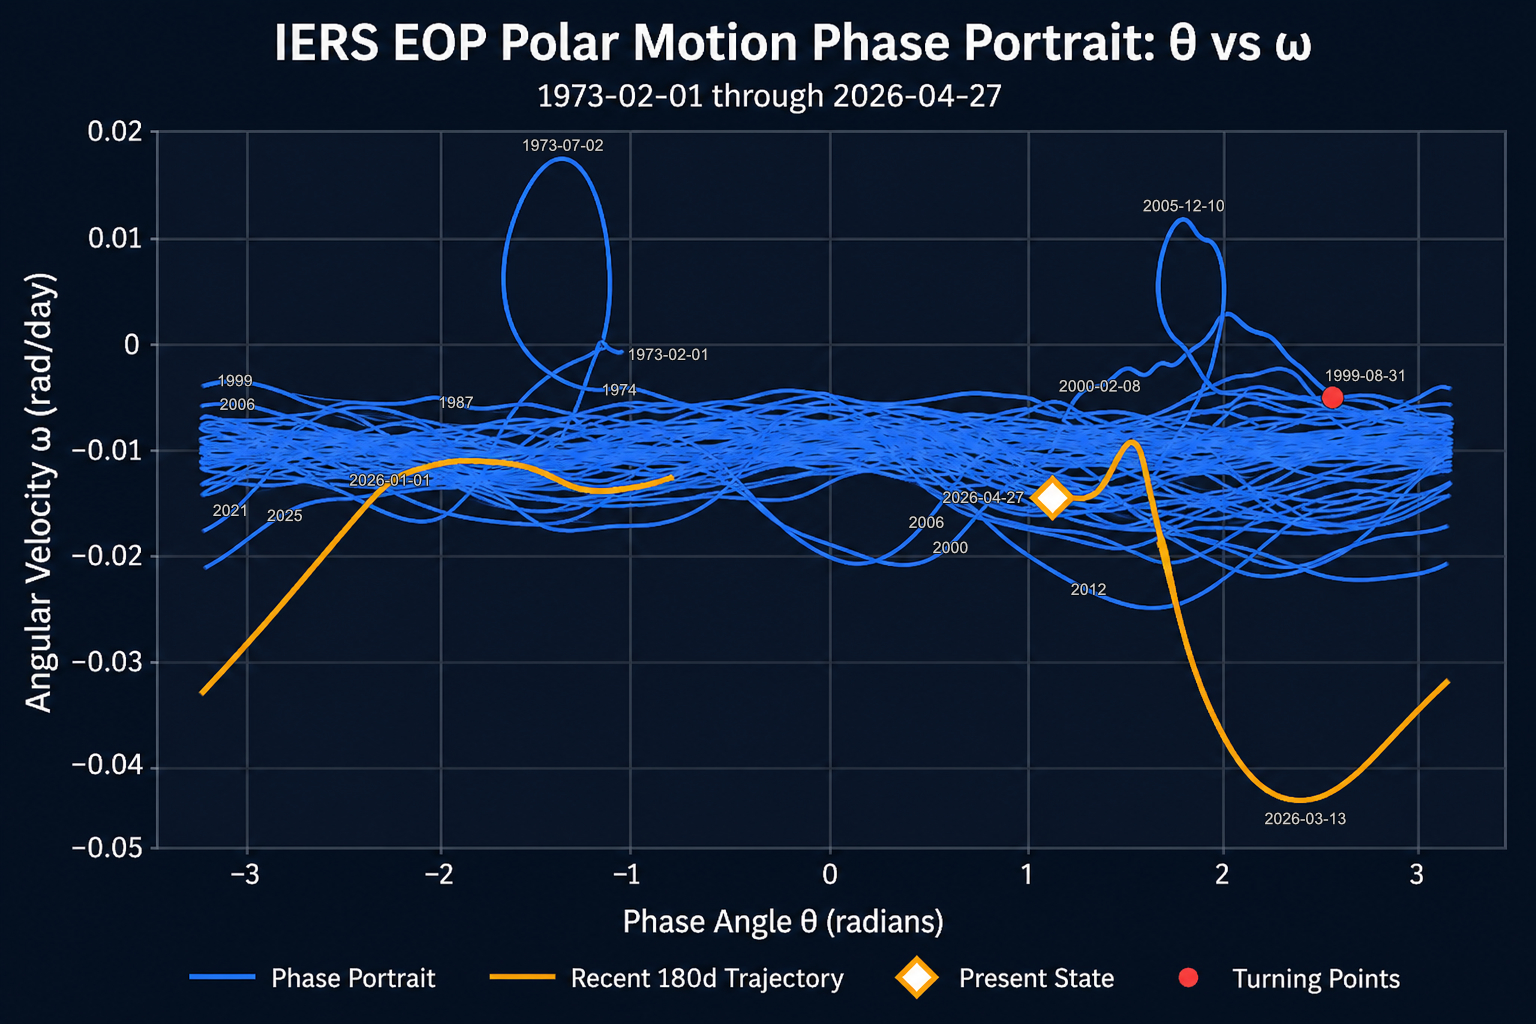
\includegraphics[width=\textwidth]{outputs/eoportrait.jpg}
\caption{\textbf{IERS EOP polar-motion phase portrait, 1973--2026.} The figure plots the angular phase coordinate $\theta$ of the polar-motion state against its angular velocity $\omega$, using IERS Earth Orientation Parameters from 1973-02-01 through 2026-04-27. The full historical trajectory is shown in blue, while the most recent 180-day trajectory is highlighted in orange. The present state is marked by the white diamond. Red markers identify selected turning-point detections, including the 1999-08-31 transition emphasized in this study. Rather than forming an unconstrained cloud, the trajectory occupies a narrow, structured band in $(\theta,\omega)$ phase space, punctuated by episodic excursions and loop-like departures. The recent trajectory departs strongly from the historical band, reaching unusually negative angular velocity near 2026-03-13 before returning toward the present state. This headline phase portrait summarizes the central empirical claim of the paper: polar motion is not merely a pair of independent coordinate time series, but a low-dimensional rotational state variable whose geometry exposes regime changes, metastable excursions, and possible leading indicators of drift transitions.}
\label{fig:eop-phase-portrait}
\end{figure*}

\section*{Plain-Language Summary}

The position of Earth’s rotation axis relative to its surface—known as polar motion—is
usually explained by adding together many physical effects, such as atmospheric winds,
ocean circulation, and changes in ice mass. In this study, we take a different approach.
Instead of starting with assumed causes, we first ask what structure is directly required
by the observed data itself.

By analyzing the geometry of polar motion over the period covered by available observations,
we find that the motion is not random. Instead, it is confined to a low-dimensional shape
and organized around a dominant direction. When projected onto this direction, the motion
separates into two distinct states, with the system switching intermittently between them.
The dynamics show bursts of rapid change and periods of persistence, indicating structured,
non-random transitions between preferred configurations.

Examining the residual motion in phase space reveals a more detailed picture. The trajectory
forms repeated looping patterns, corresponding to a quasi-periodic oscillation, while
simultaneously drifting along a preferred path. These loops are not stationary: their
centers evolve over time, tracing a slow, continuous trajectory that does not repeat.
The rate of this slow evolution varies substantially, including periods of acceleration,
deceleration, and temporary reversal. This shows that the system is not governed by a
single long-period cycle, but instead evolves on a time-dependent geometric structure.

Taken together, these observations indicate that polar motion consists of coupled dynamics:
a faster oscillatory component embedded within a slower, nonstationary drift. The system
therefore behaves as a low-dimensional dynamical process with two preferred states, in
which motion circulates locally while the overall structure evolves over time.

To test whether these patterns are meaningful, we apply a series of robustness checks.
These include varying the level of smoothing, changing how states are defined, and
comparing the results with synthetic datasets that mimic correlated noise. The geometric
features—such as low-dimensional confinement, bistability, and the coupled oscillatory–
drift structure—remain stable under all tests. However, the strength and stability of any
specific direction are not statistically distinguishable from what can arise in correlated
random processes.

Importantly, these results describe the geometric constraints evident within the time
interval sampled by the available data, and do not imply that the same structure must
hold outside this observational window.

This leads to a refined interpretation. Polar motion appears as a low-dimensional, bistable system with coupled fast and slow dynamics, in which oscillatory motion is embedded within a drifting geometric framework. While the geometry of this behavior is robustly supported by the data, its directional features may emerge naturally from internally correlated dynamics rather than from a fixed external alignment.

In the expanded analysis, this intrinsic geometry is compared with lagged planetary torque-phase proxies. The resulting relationship is not treated as direct deterministic forcing. Rather, the evidence is framed as phase conditioning: external gravitational geometry appears to modulate the probability of high-deviation states and state transitions within an already structured, metastable rotational system.

In compact form, the system occupies a low-dimensional, bistable manifold in which oscillatory trajectories are advected along a nonstationary slow manifold.

\section{Abstract}
\label{sec:abstract}
\begin{abstract}

We analyze polar motion as a geometric dynamical system using a constraint-first methodology, focusing on invariant structure rather than imposed physical models. Using filtered polar motion data, we identify a persistent low-dimensional organization characterized by near-planar confinement, a dominant principal axis, and a robust two-state (bistable) structure in projected coordinates.

A comprehensive robustness framework is applied, including smoothing sensitivity analysis, threshold invariance tests, and colored-noise (AR(1)) surrogate comparisons. The geometric structure—specifically planar confinement and bistability—is shown to be stable across all smoothing scales and thresholding methods. However, the magnitude of absolute (Earth-fixed) directional anisotropy and apparent axis stability are not statistically distinguishable from correlated stochastic processes under AR(1) and rotational null models.

These results support a refined interpretation: polar motion exhibits a low-dimensional, bistable geometric organization that is intrinsic to the data, while its directional features may emerge from temporally correlated dynamics rather than fixed external constraints. This reframes prior interpretations of Earth-fixed structure as emergent rather than imposed.

In compact form, the system can be described as a low-dimensional, bistable manifold in which oscillatory trajectories evolve within, and are advected by, a nonstationary slow mode. The present expanded manuscript further tests whether transition probabilities within this manifold are conditioned by planetary torque-phase geometry. Lagged enrichment, phase-sector localization, and escape-rate diagnostics are interpreted conservatively as evidence for weak phase-conditioned modulation rather than deterministic planetary forcing, consistent with metastable escape theory and nonequilibrium dynamical systems.

\end{abstract}

\section{Introduction}
\label{sec:introduction}

Polar motion represents the displacement of the Earth's rotation axis relative to its crust and is a fundamental observable in geodesy and Earth system dynamics. Traditionally, it is interpreted as the superposition of known physical components, including the Chandler wobble, annual forcing, and residual excitation attributed to atmosphere, oceans, and hydrology \citep{dickman2000,gross2007}.

While these models have been successful in reproducing broad spectral characteristics, they are inherently constructive: they explain the signal through the aggregation of assumed mechanisms. In contrast, the present study adopts a constraint-first approach, seeking to identify geometric invariants in the observed data prior to any dynamical or physical interpretation.

This distinction is critical. Rather than asking which mechanisms produce polar motion, we ask:

\begin{quote}
What geometric structure is required by the data itself?
\end{quote}

Recent work has suggested that polar motion may exhibit low-dimensional organization and state-like behavior beyond simple harmonic superposition. In particular, analyses of residual polar motion have revealed clustering, directional persistence, and apparent transitions between preferred configurations. However, the interpretation of these features remains ambiguous: they may reflect genuine dynamical structure, or they may arise from correlated stochastic processes.

The central objective of this study is therefore to separate:
\begin{enumerate}
    \item \textbf{Geometric constraints} that are directly supported by the data, and
    \item \textbf{Statistical interpretations} that depend on the choice of null model.
\end{enumerate}

To this end, we perform a systematic geometric analysis of filtered polar motion time series, focusing on:

\begin{itemize}
    \item Dimensionality reduction and planar confinement,
    \item Principal axis structure and its temporal behavior,
    \item Projection-based state decomposition and bistability,
    \item Phase-space reconstruction and dynamical organization.
\end{itemize}

Crucially, we augment this analysis with a dedicated robustness framework designed to test whether inferred structures persist under:
\begin{enumerate}
    \item Variations in smoothing scale,
    \item Alternative state definitions (mean, median, clustering),
    \item Colored-noise surrogate models (AR(1)),
    \item rotational null models for axis stability.
\end{enumerate}

This allows us to distinguish between:
\begin{itemize}
    \item \emph{Invariant geometric structure}, and
    \item \emph{Apparent structure induced by temporal correlation or statistical artefacts}.
\end{itemize}

The results show that polar motion is well described by a low-dimensional geometric manifold with a robust two-state organization. However, directional anisotropy and apparent axis stability are not statistically distinguishable from appropriately constructed null models. This leads to a revised interpretation in which the system's geometry is intrinsic, while its directional features may emerge from correlated stochastic dynamics rather than fixed external forcing.

\paragraph{Hierarchy of Inference.}
To maintain a clear separation between observation and interpretation, results are organized into three tiers:

\begin{itemize}
\item \textbf{Tier 1: Geometric invariants} — properties that remain stable under all preprocessing and surrogate tests (e.g., low-dimensional confinement, planar structure, bistability),
\item \textbf{Tier 2: Dynamical organization} — robust but interpretive features inferred from phase-space structure (e.g., coupled fast--slow dynamics, loop structure, drift),
\item \textbf{Tier 3: Directional features} — quantities sensitive to null-model choice and therefore interpreted cautiously (e.g., anisotropy magnitude, axis stability).
\end{itemize}

This hierarchy ensures that conclusions reflect the strength of empirical support rather than presentation order.

This paper is organized as follows. Section~\ref{sec:introduction} describes the data and preprocessing steps. Section~\ref{sec:methods} outlines the geometric analysis framework. Section~\ref{sec:results} presents the results, including dimensionality reduction, state structure, and phase-space reconstruction. Section~\ref{sec:methods} introduces robustness diagnostics and evaluates statistical significance under multiple null models. Section~\ref{sec:discussion} discusses the implications for interpreting polar motion as a dynamical system.



\section{Conceptual Framework}
\label{sec:conceptual_framework}

We distinguish three layers of description.

\subsection{Geometric Constraint}
\label{subsec:geometric_constraint}

The observed polar motion is confined to a low-dimensional manifold embedded in the full state space. This constraint is independent of any dynamical model and arises directly from the data.

\subsection{Intrinsic Dynamics}
\label{subsec:intrinsic_dynamics}

Within this manifold, the system exhibits bistability, characterized by two preferred states, intermittent transitions, phase-space looping structure, and slow drift of loop centers. These properties are consistent with a weakly coupled, noise-activated system evolving on a reduced manifold \citep{prigogine1984,kramers1940,risken1989}.

\subsection{External Phase Conditioning}
\label{subsec:external_phase_conditioning}

The new contribution of this expanded work is the identification of a statistically structured relationship between transition behavior and planetary torque phase. This is not formulated as a claim that planetary torques continuously drive polar motion. Instead, the working interpretation is narrower: planetary geometry may condition the effective probability landscape within which transitions occur. Classical excitation theory remains relevant for forcing amplitudes and angular-momentum exchange \citep{munk1960,lambeck1980,dickman2000,gross2007}, while the present analysis asks whether a low-dimensional Earth-rotation state space is also sensitive to the phase geometry of the solar-system torque environment \citep{murraydermott1999}.

\section{Results}
\label{sec:results}
\label{sec:results}

\noindent\textit{Analytical procedures, filtering choices, and surrogate constructions are detailed in Section~\ref{sec:methods}.}

\subsection{Planar Structure and Principal Axis}
\label{subsec:planar_structure_and_principal_axis}

The polar motion trajectory in $(x,y)$ space exhibits strong directional organization (Figure~\ref{fig:trajectory}), with motion confined to a narrow band rather than isotropically distributed.

\begin{figure}[h!]
\centering
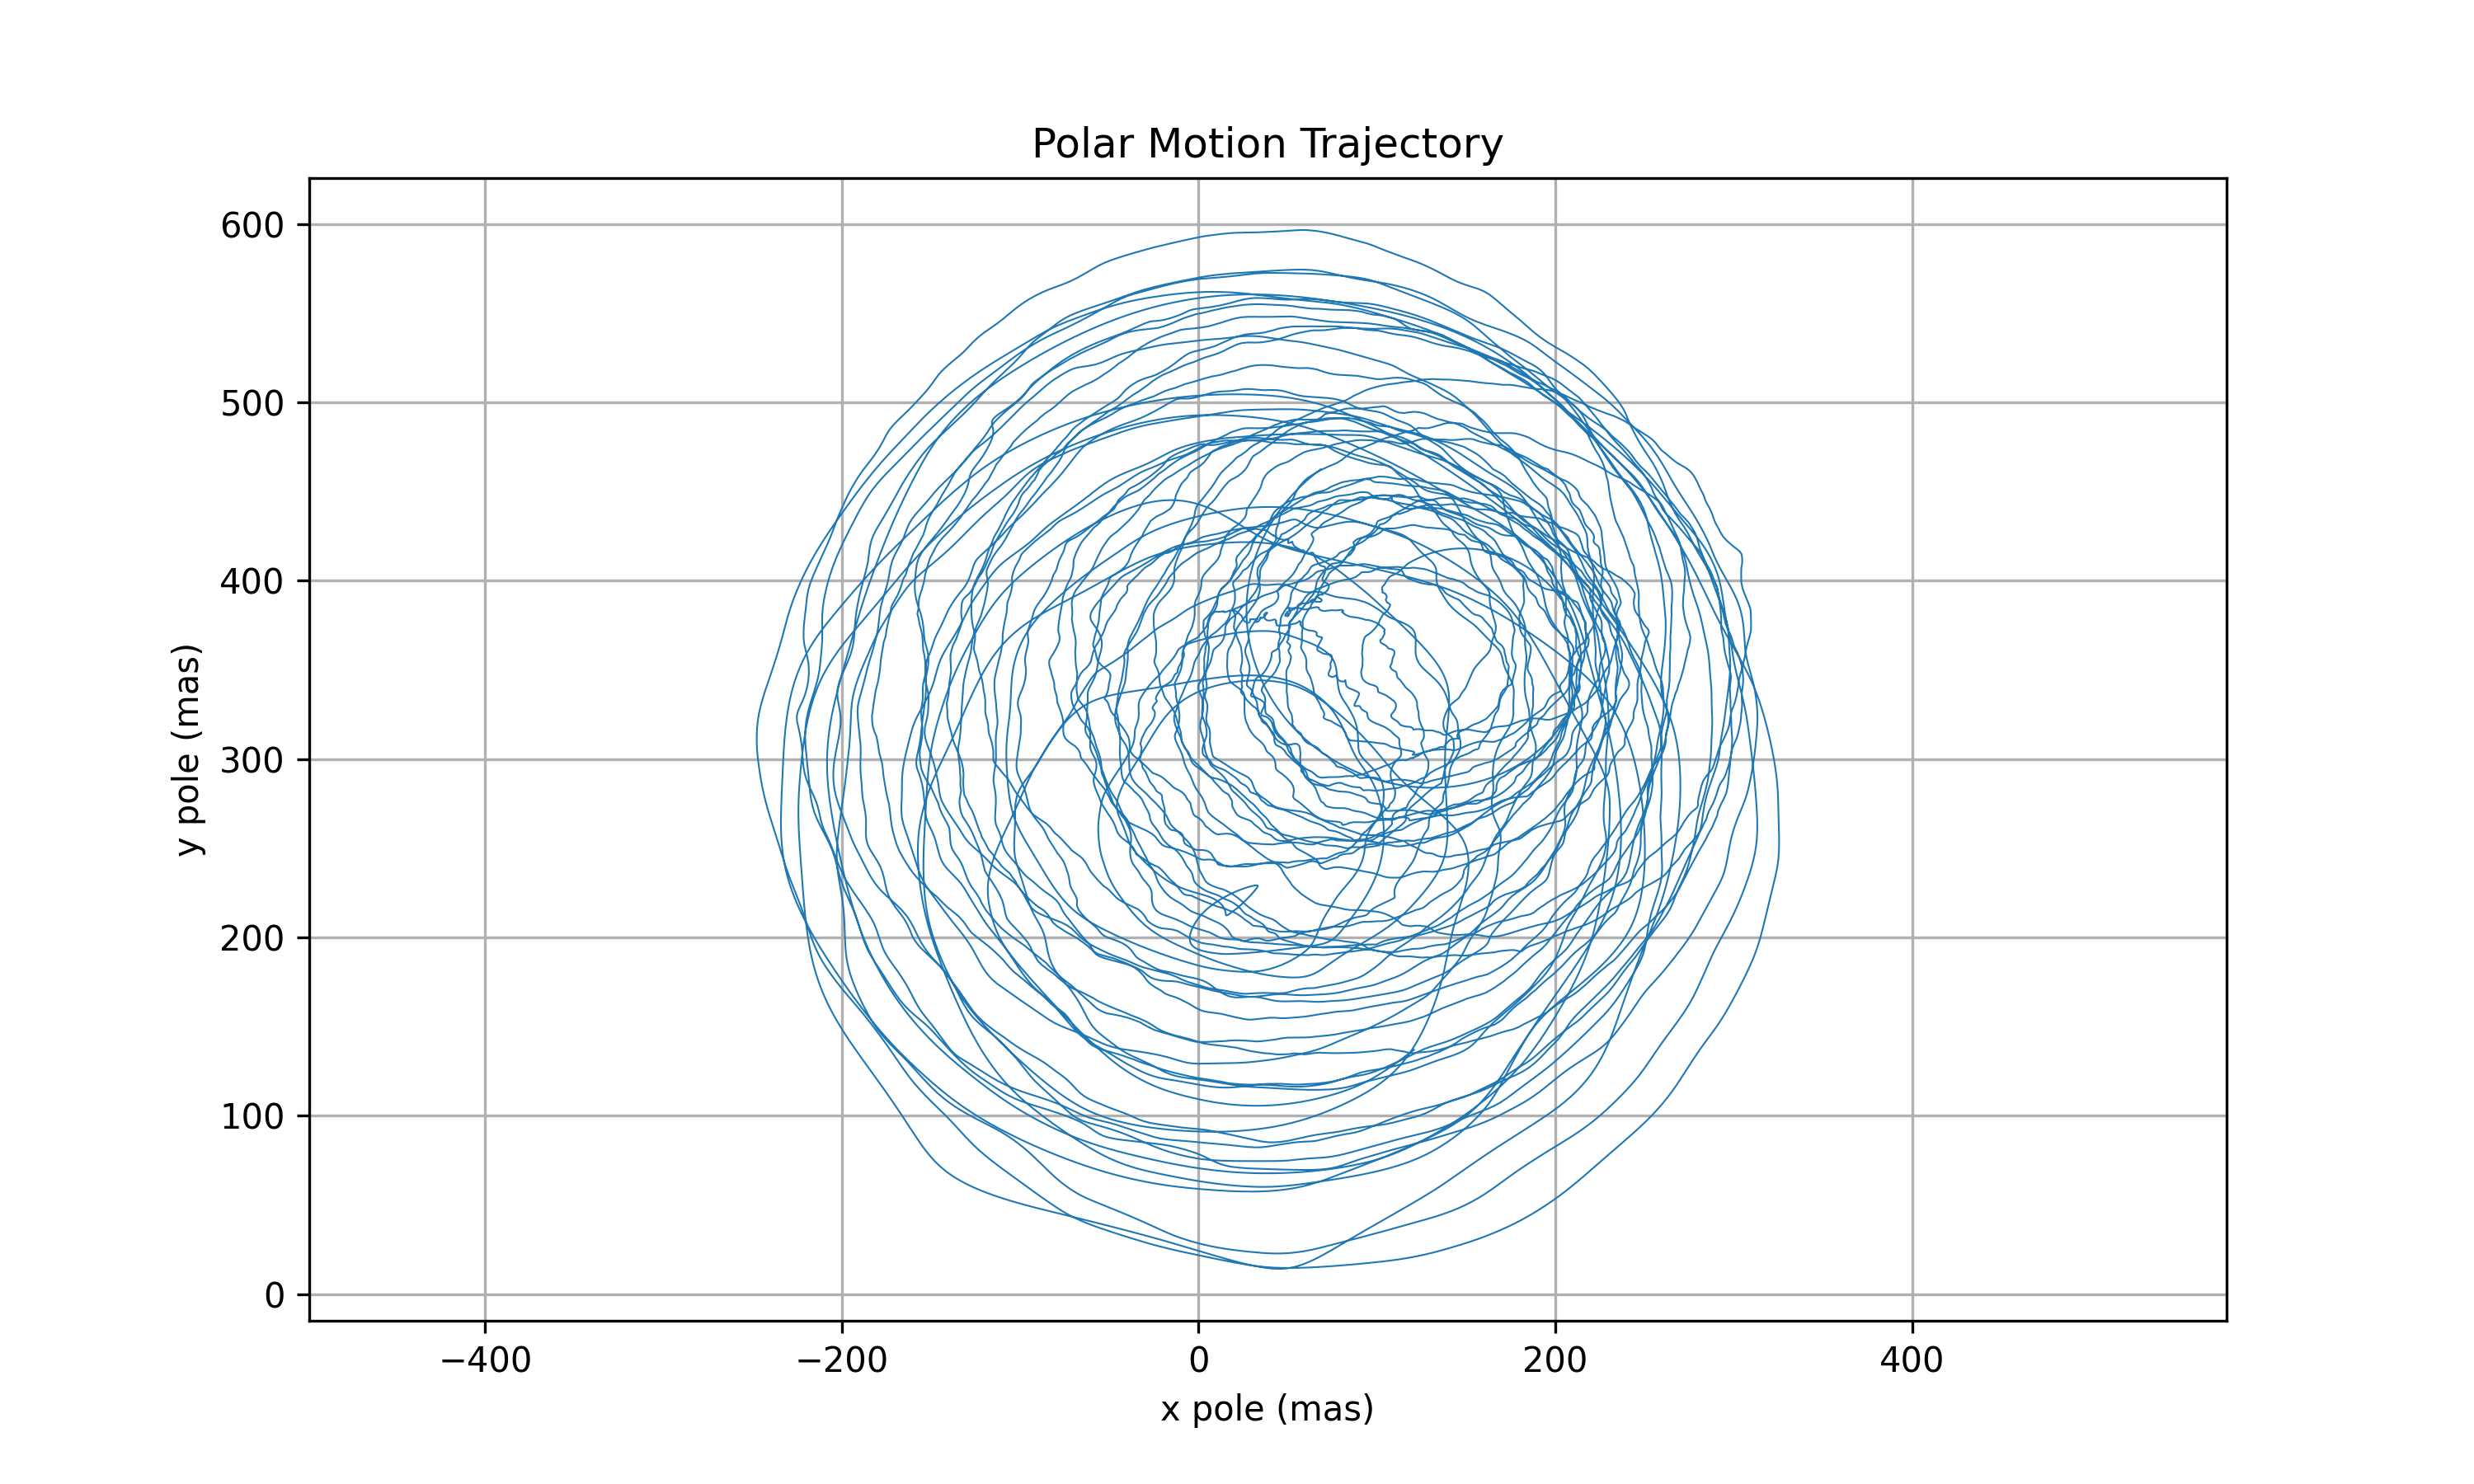
\includegraphics[width=0.5\textwidth]{fig_01_polar_trajectory.png}
\caption{Polar motion trajectory in $(x,y)$ space showing strong directional confinement.}
\label{fig:trajectory}
\end{figure}

The corresponding velocity field (Figure~\ref{fig:vector_field}) reveals coherent flow aligned with a dominant direction.

\begin{figure}[h!]
\centering
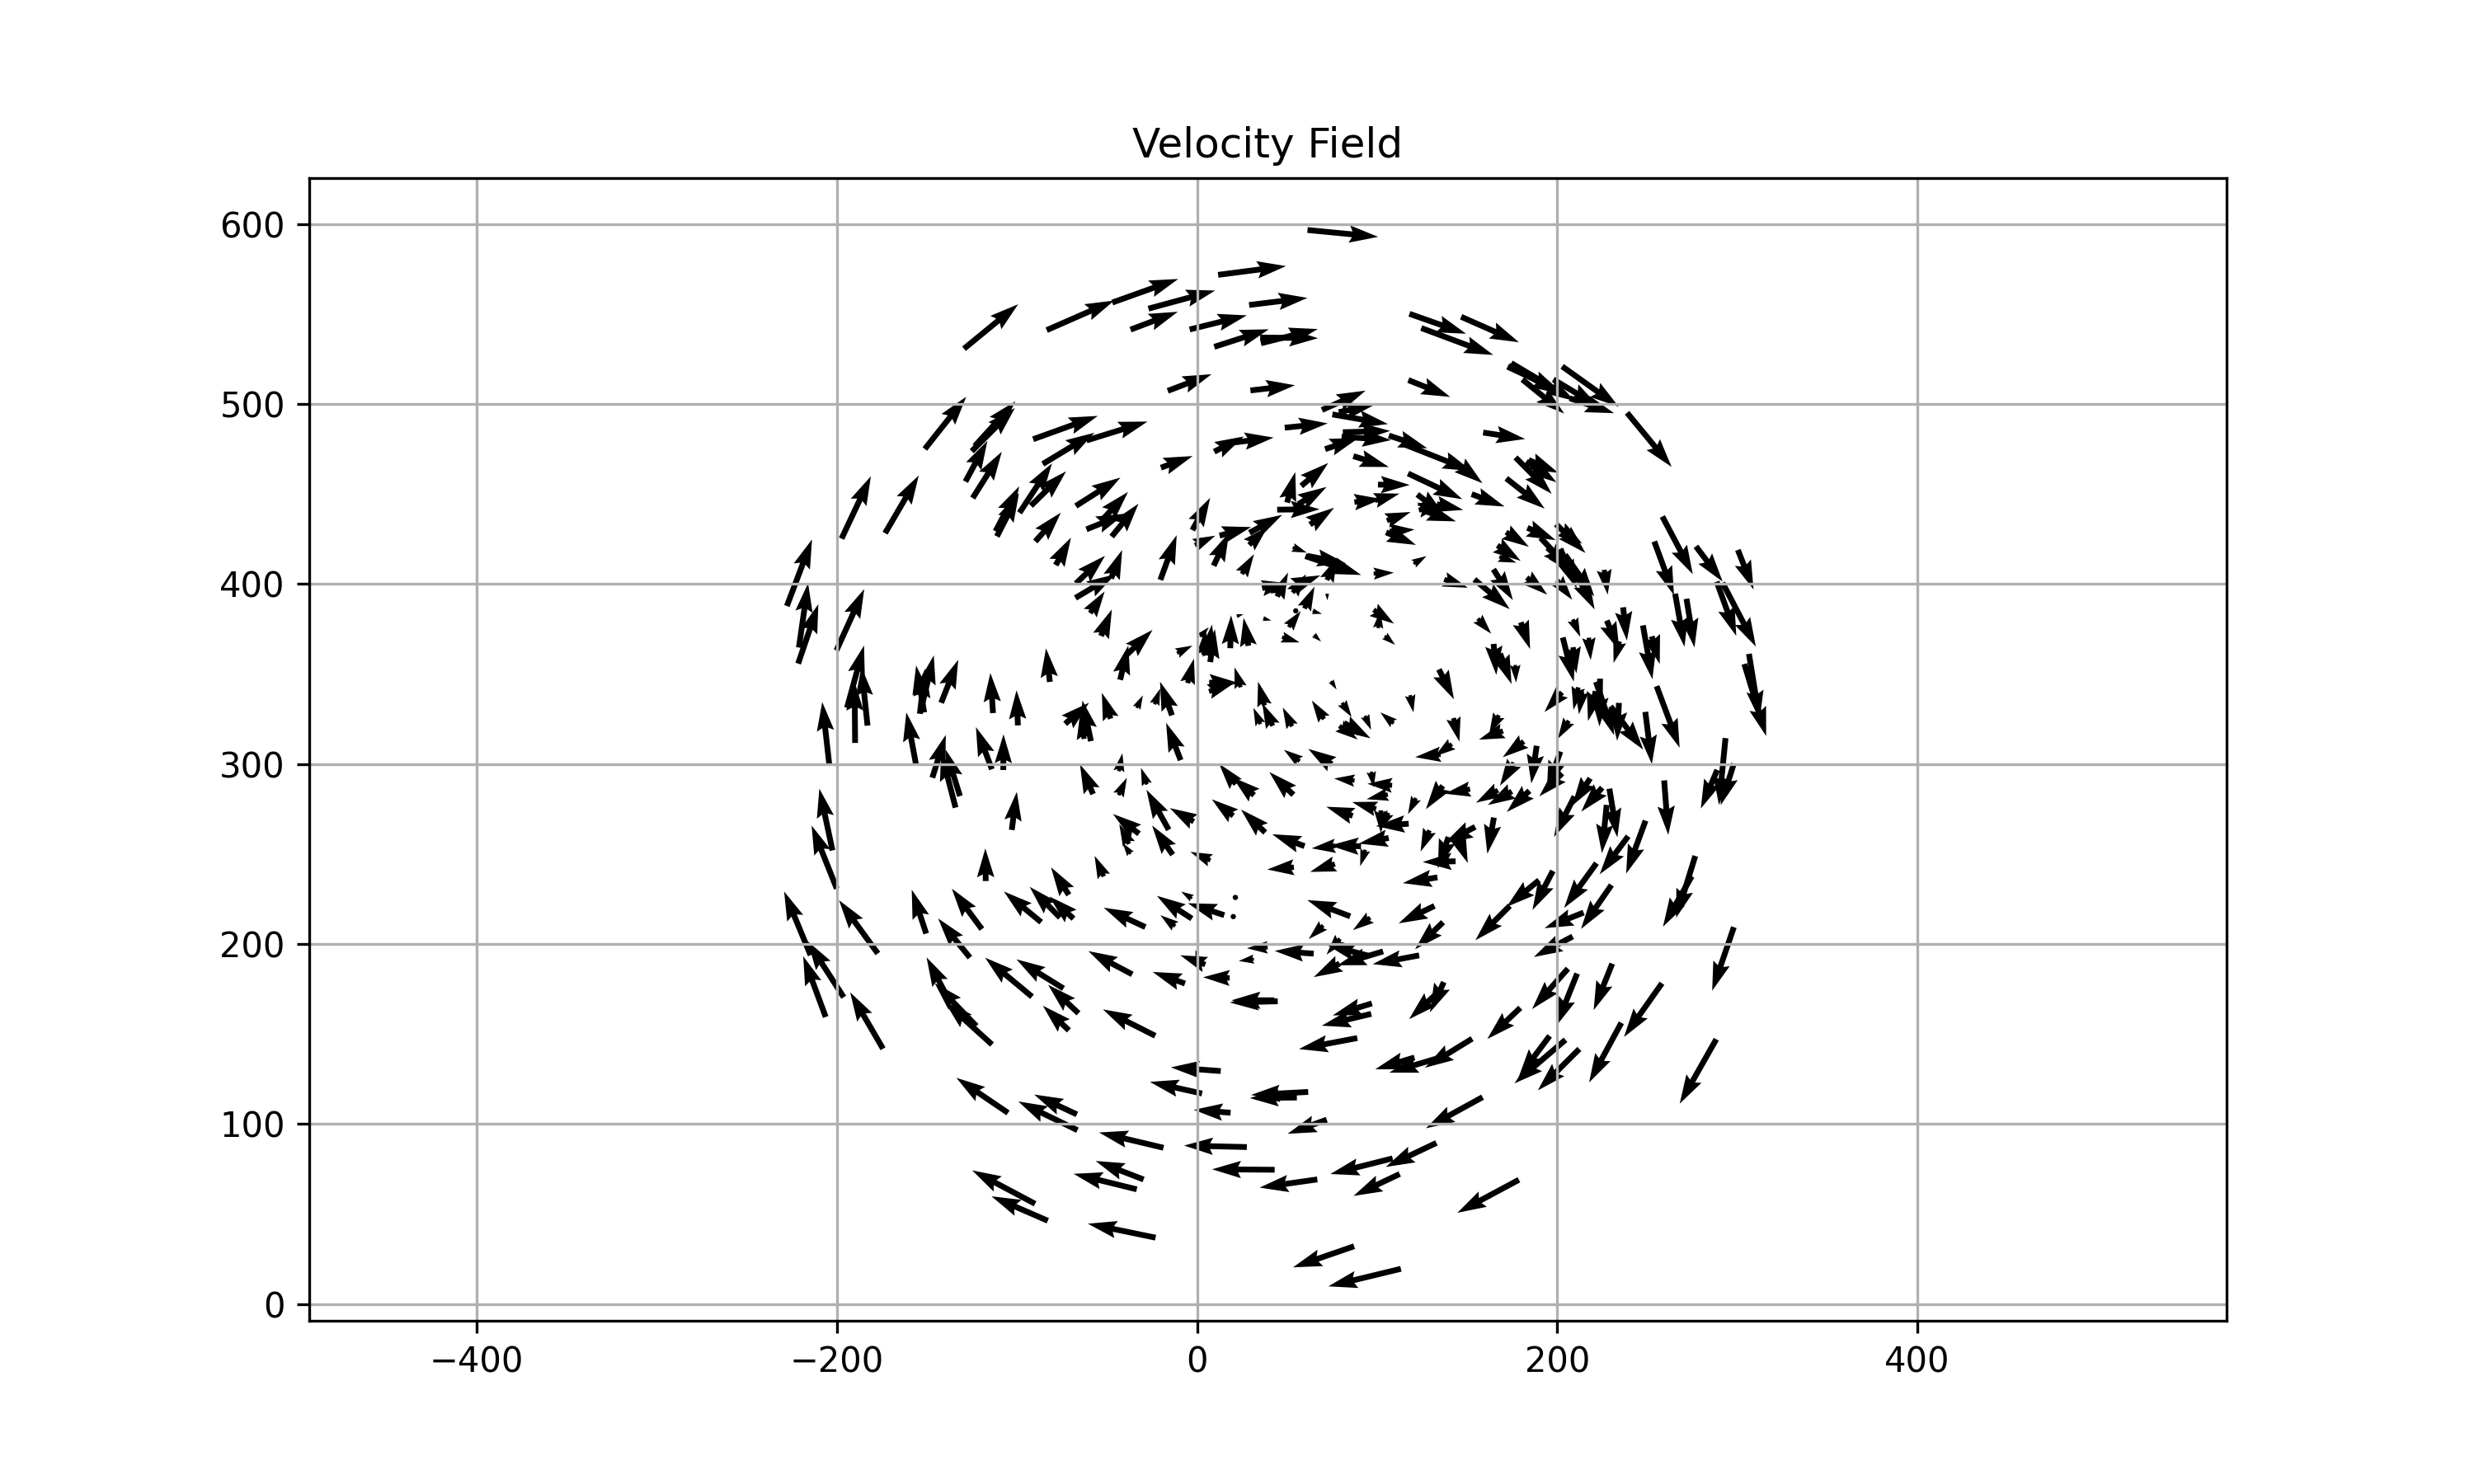
\includegraphics[width=0.5\textwidth]{fig_02_vector_field.png}
\caption{Velocity vector field illustrating coherent directional flow.}
\label{fig:vector_field}
\end{figure}

Principal component analysis shows that variance is strongly concentrated along a single axis (Figure~\ref{fig:pca}), indicating effective dimensional reduction.

\begin{figure}[h!]
\centering
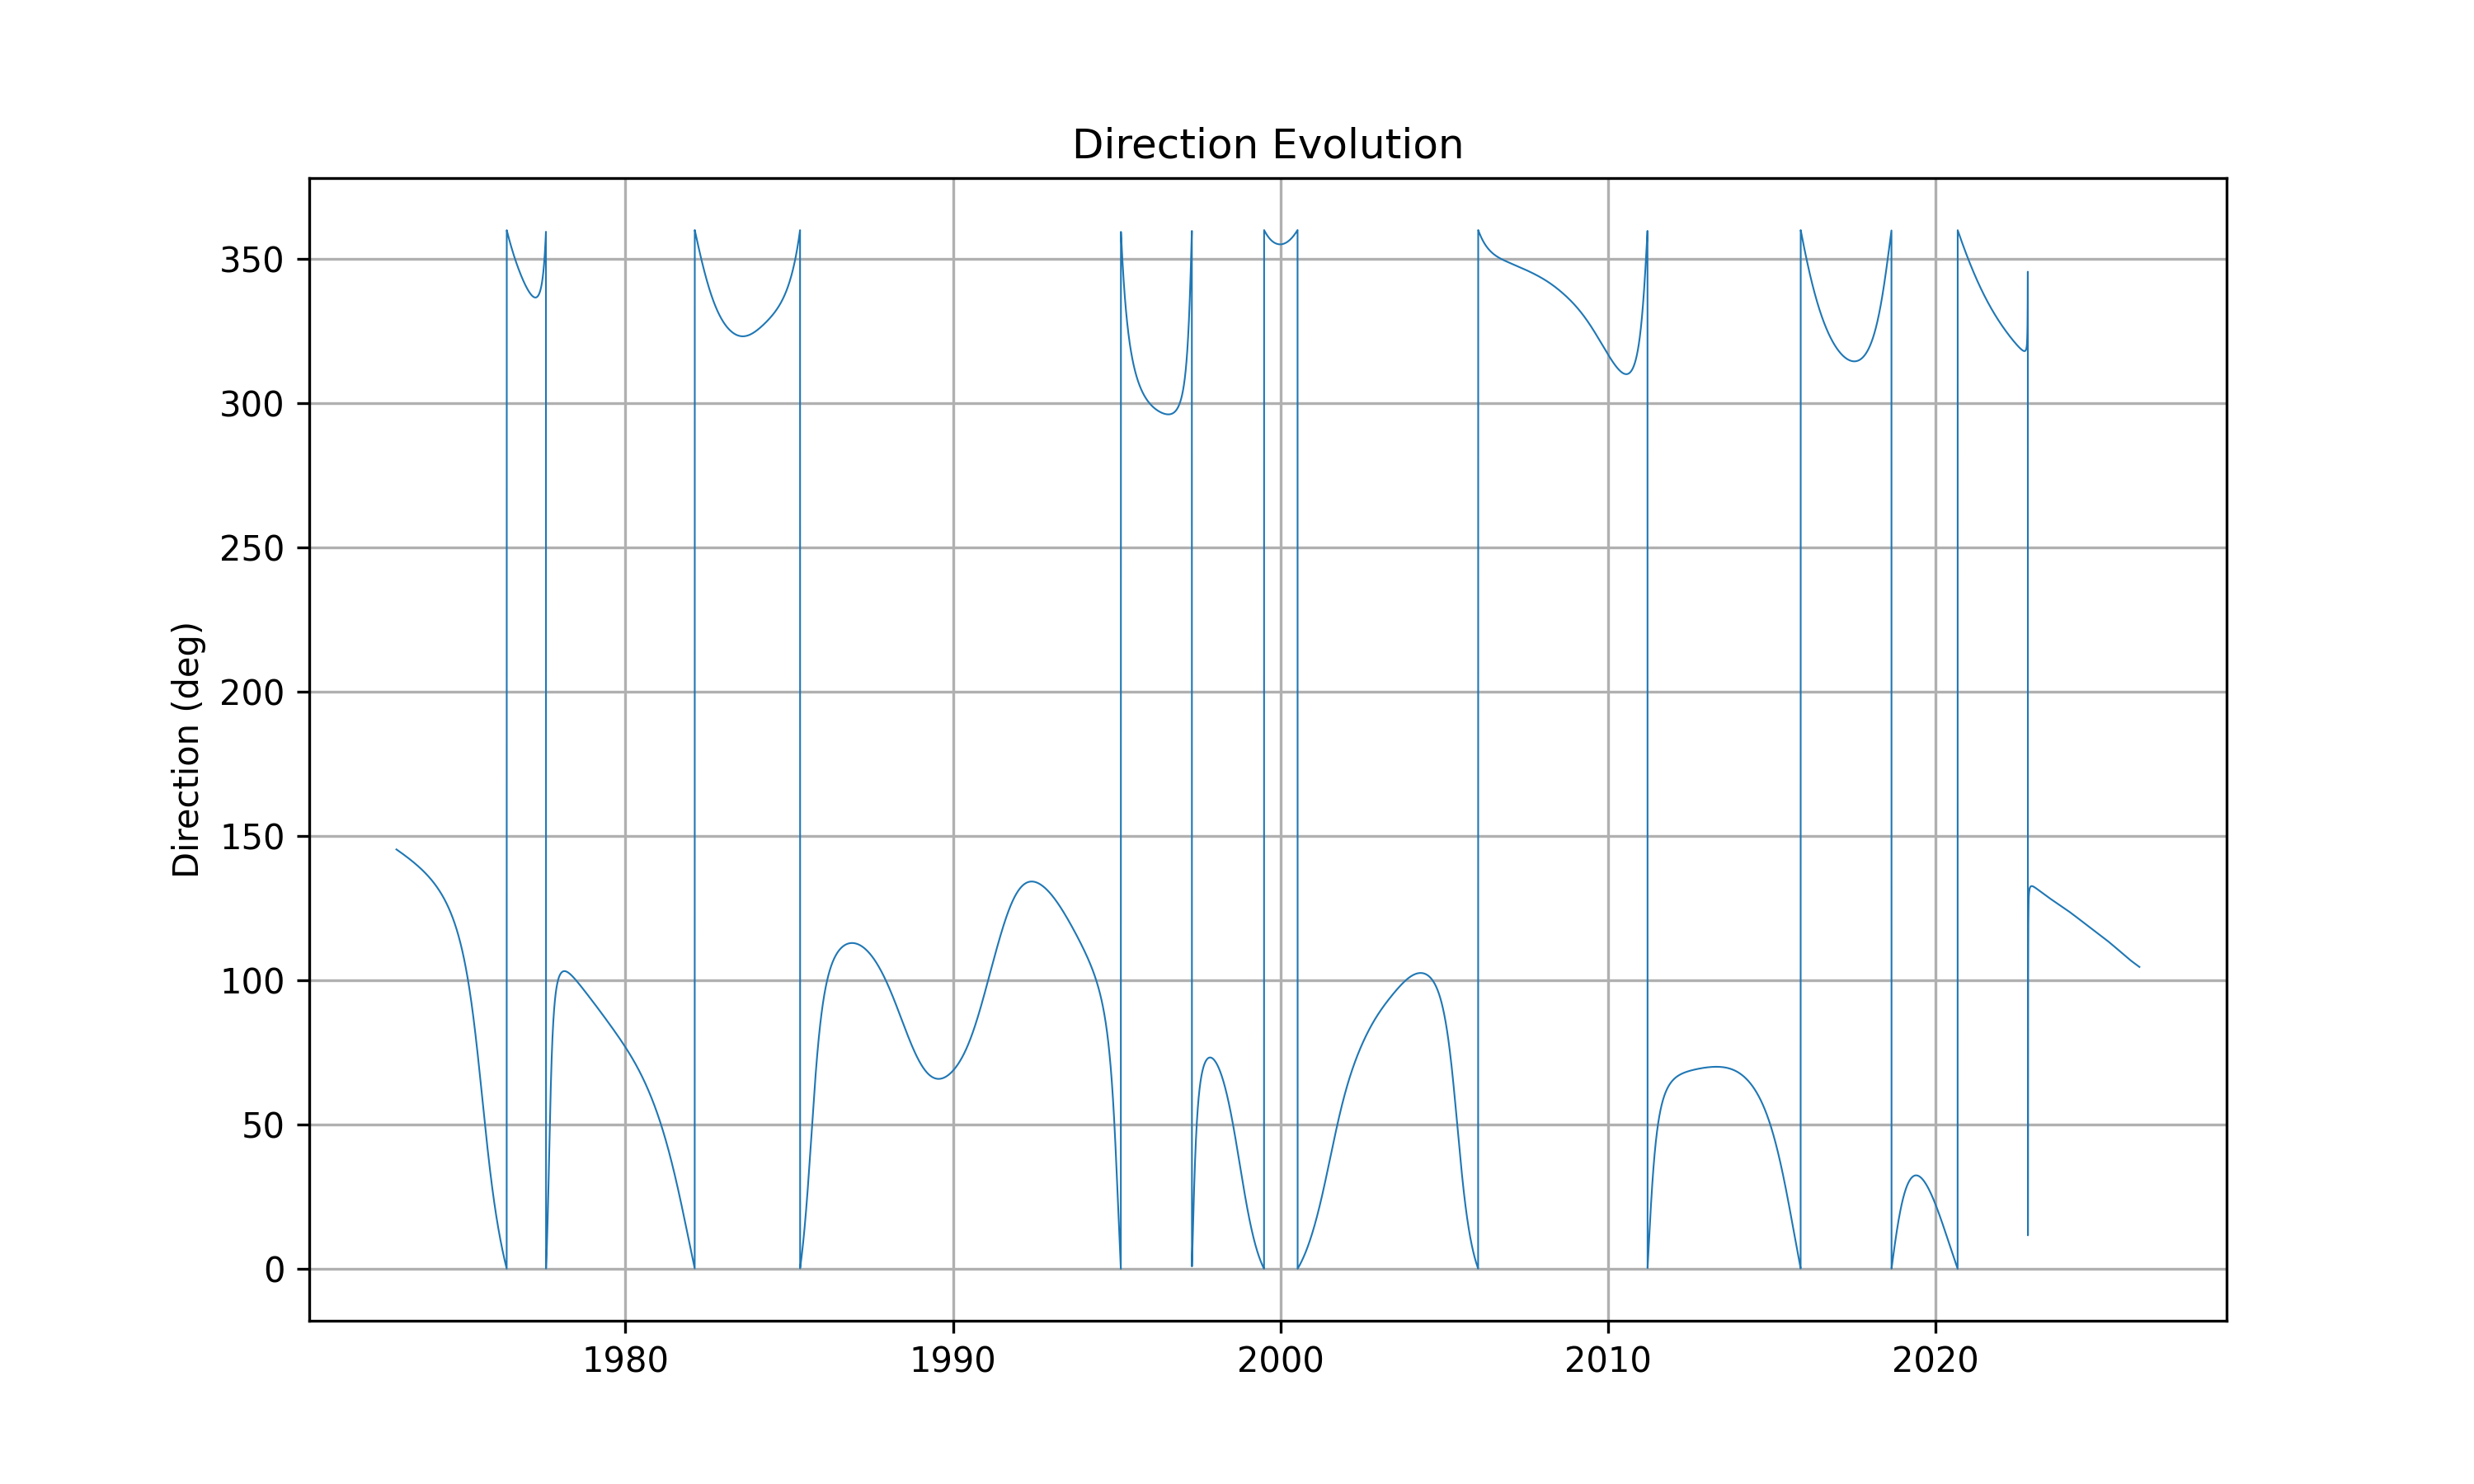
\includegraphics[width=0.5\textwidth]{fig_03_direction_time.png}
\caption{Principal component decomposition showing dominance of a single axis.}
\label{fig:pca}
\end{figure}

The variance ratio (Figure~\ref{fig:variance_ratio}) confirms that the system is well approximated by a low-dimensional structure.

\begin{figure}[h!]
\centering
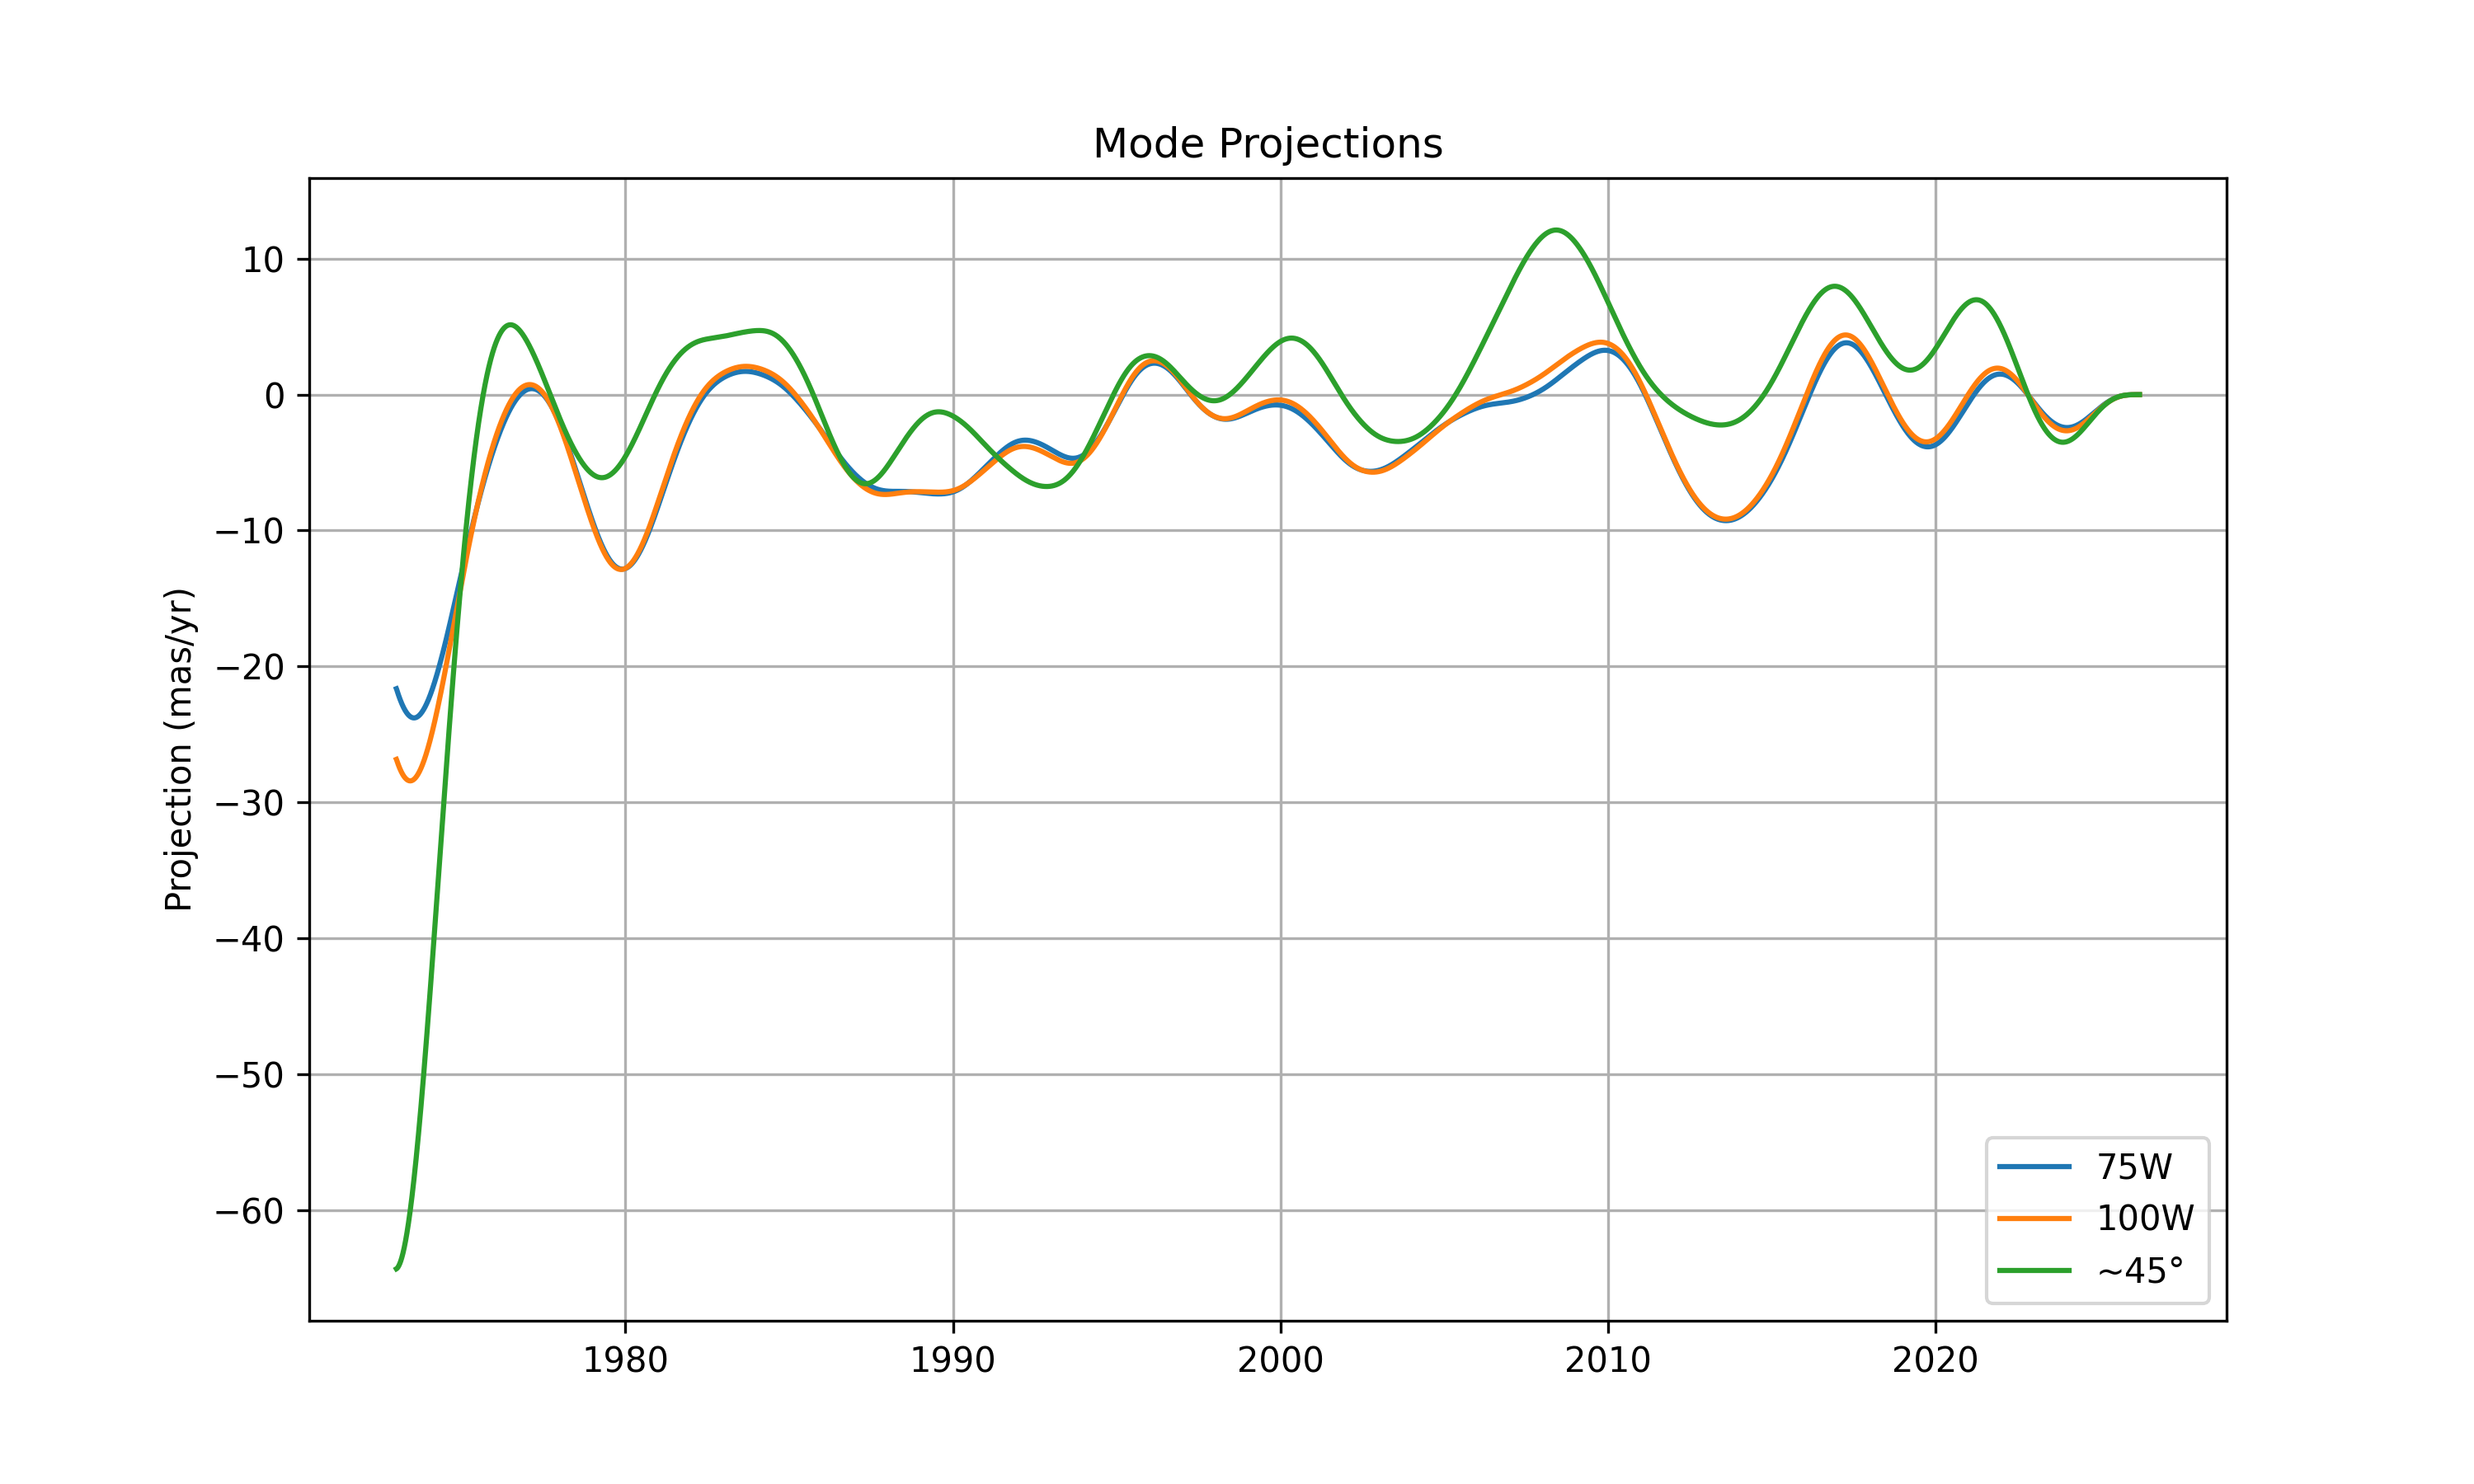
\includegraphics[width=0.5\textwidth]{fig_04_mode_projections.png}
\caption{Principal-axis projections across smoothing windows (75W, 100W, and ~45-day equivalent). The curves represent trajectory projections onto the dominant eigenvector, not variance ratios.}
\label{fig:variance_ratio}
\end{figure}

Across all smoothing scales tested, the orientation of the principal axis varies by less than $\sim 1.2^\circ$, and anisotropy remains stable to within $\sim 0.002$. This indicates that the observed geometric structure is not sensitive to filtering choices.

\paragraph{Observed Structural Invariance.}
Across all smoothing windows examined (45-day equivalent, 75-day, 100-day), the dominant principal axis remains stable in orientation, and the projected trajectory retains a consistent low-dimensional structure. While the amplitude and temporal coherence of the projections vary with filtering scale, the geometric alignment of the dominant mode is invariant under these transformations.

This invariance suggests that the identified structure reflects an underlying property of the system rather than an artifact of smoothing or temporal aggregation. However, the temporal ordering and transition dynamics remain sensitive to filtering choices, and are therefore treated separately.

\subsection{Interpretation of Directional Structure}
\label{subsec:interpretation_of_directional_structure}

The existence of a dominant axis reflects a persistent geometric organization of the trajectory. However, robustness testing against colored-noise surrogates shows that the magnitude of anisotropy is not statistically distinguishable from that expected under correlated stochastic dynamics.

Accordingly, the directional structure is interpreted as a geometric feature of the observed trajectory, rather than evidence of externally imposed anisotropic forcing; however, this does not preclude internally generated directional organization coupled to system dynamics.

\subsection{Two-State Structure}
\label{subsec:two_state_structure}

Projection of the trajectory onto the dominant axis reveals clear bimodal clustering (Figure~\ref{fig:state_projection}).

\begin{figure}[h!]
\centering
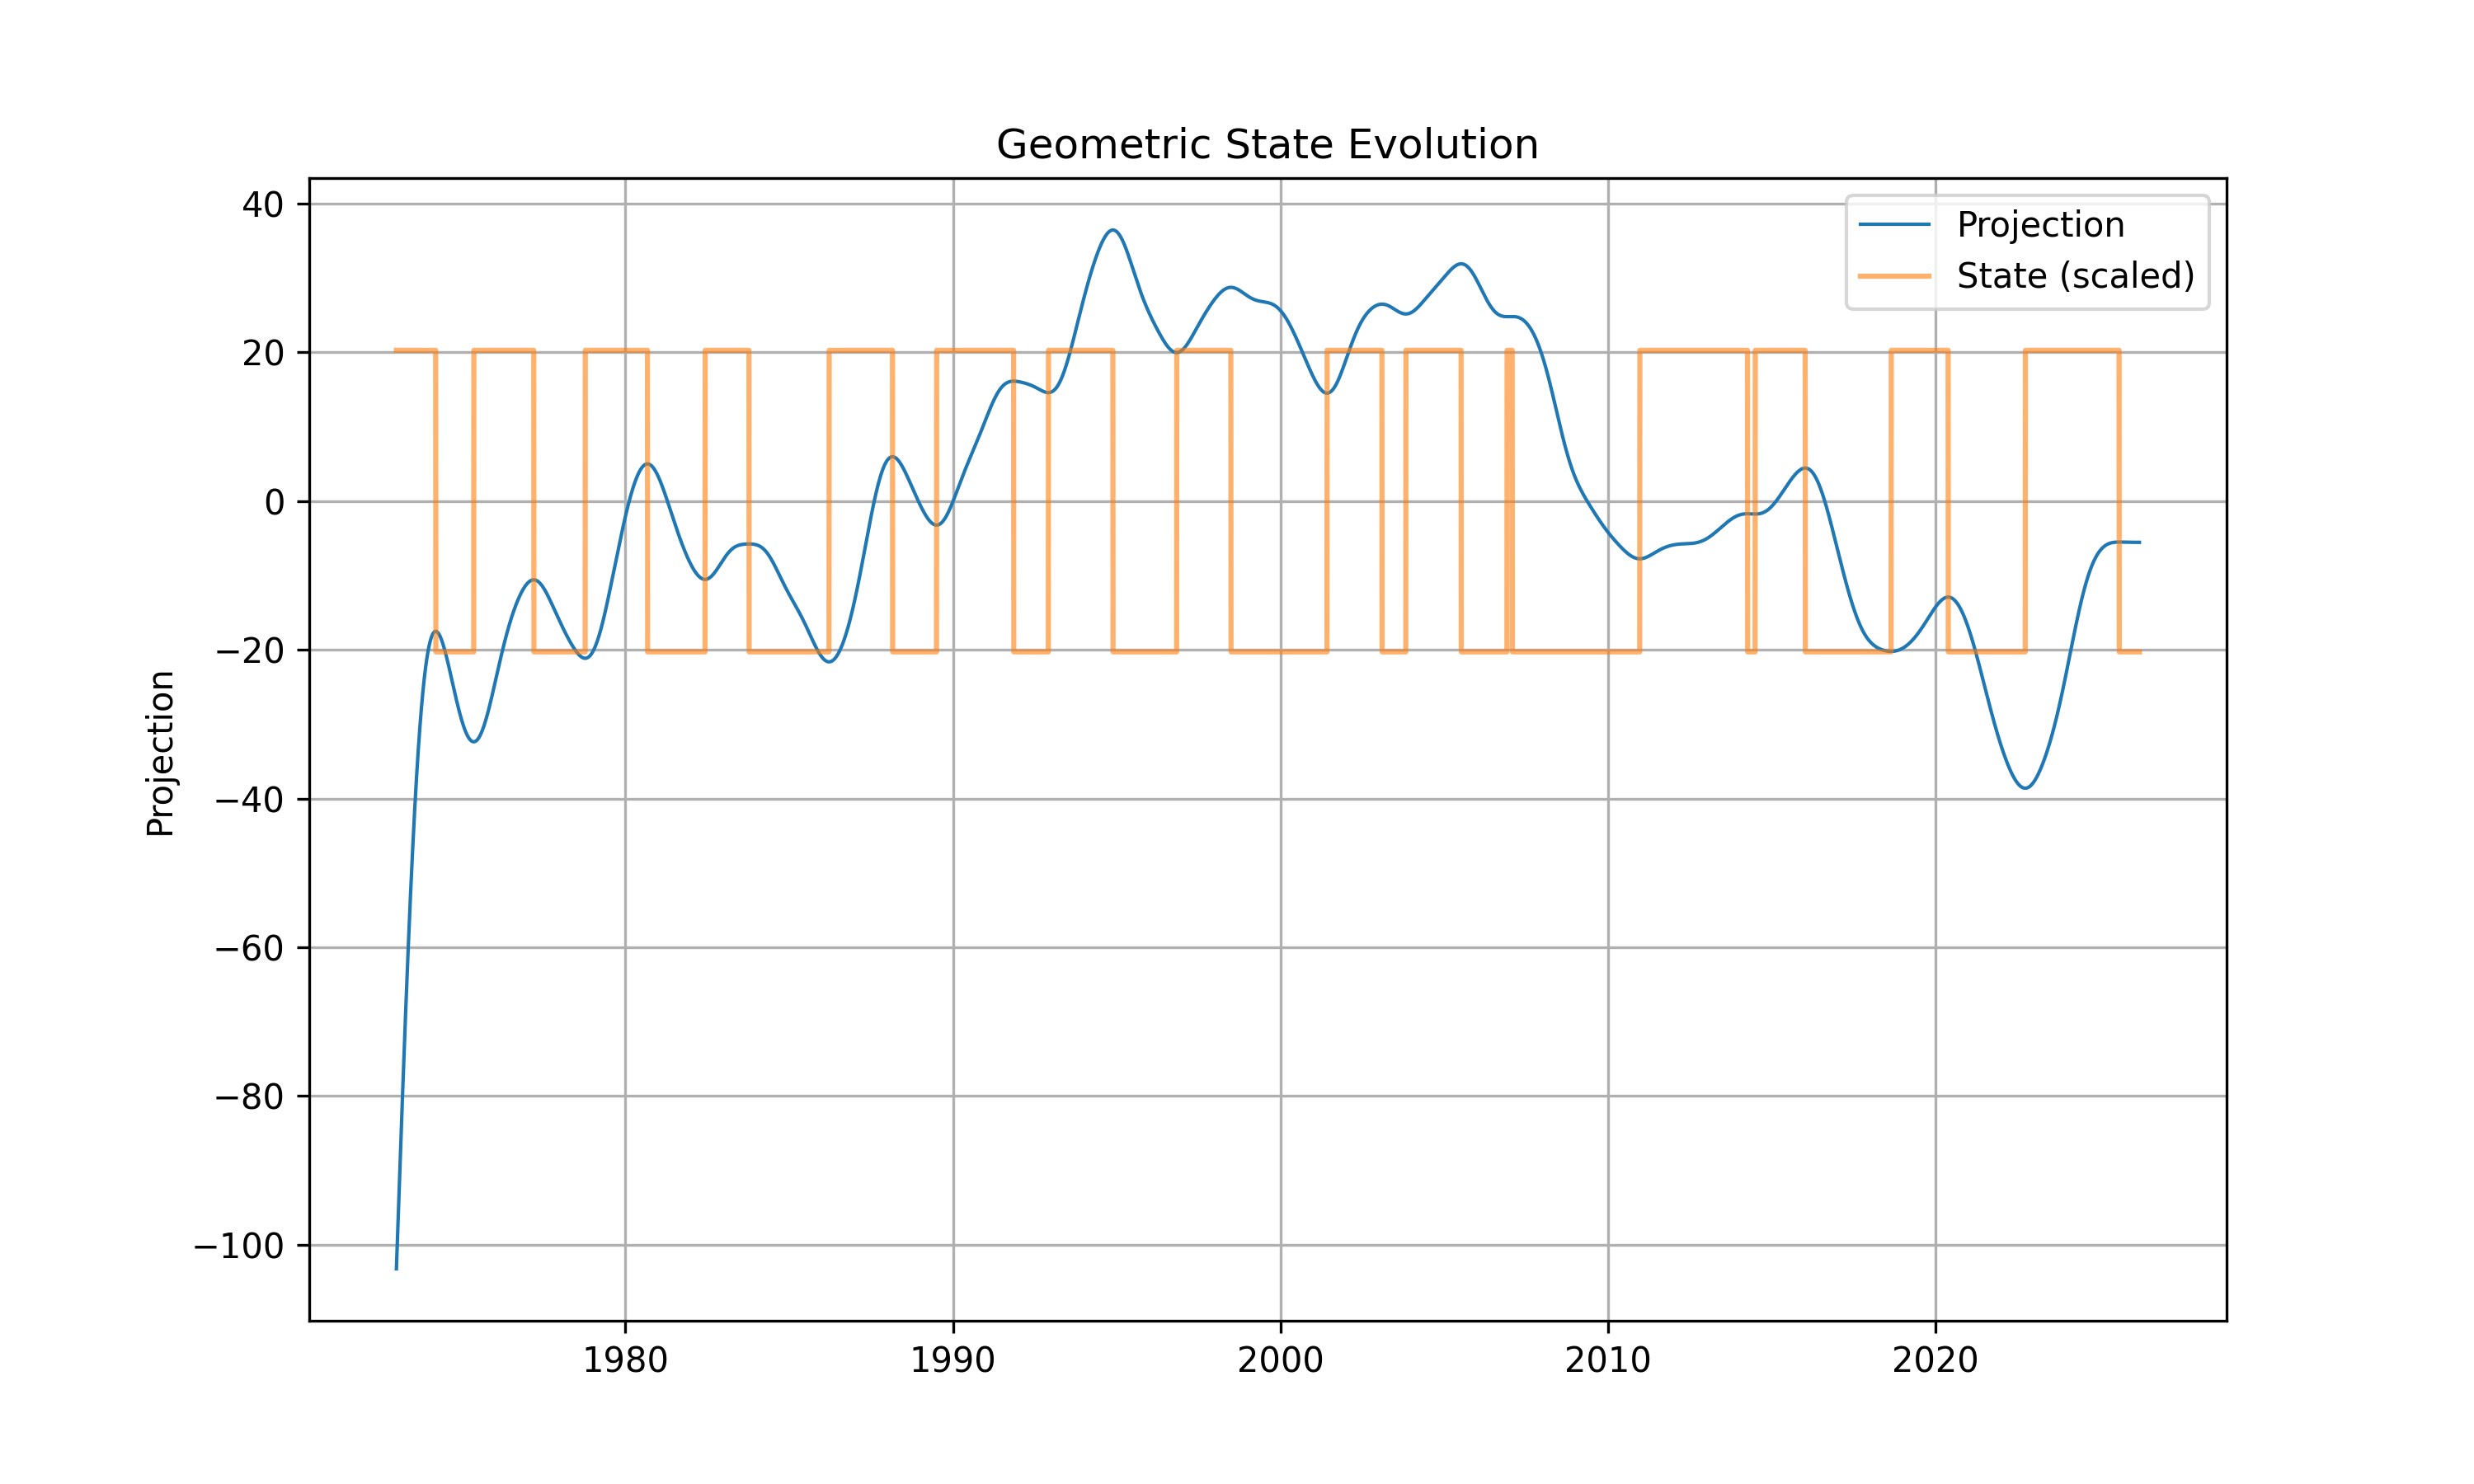
\includegraphics[width=0.5\textwidth]{fig_06_state_projection.png}
\caption{Projection onto the dominant axis showing bimodal clustering into two states.}
\label{fig:state_projection}
\end{figure}

The corresponding binary state sequence (Figure~\ref{fig:state_timeseries}) exhibits discrete transitions between two regimes.

\begin{figure}[h!]
\centering
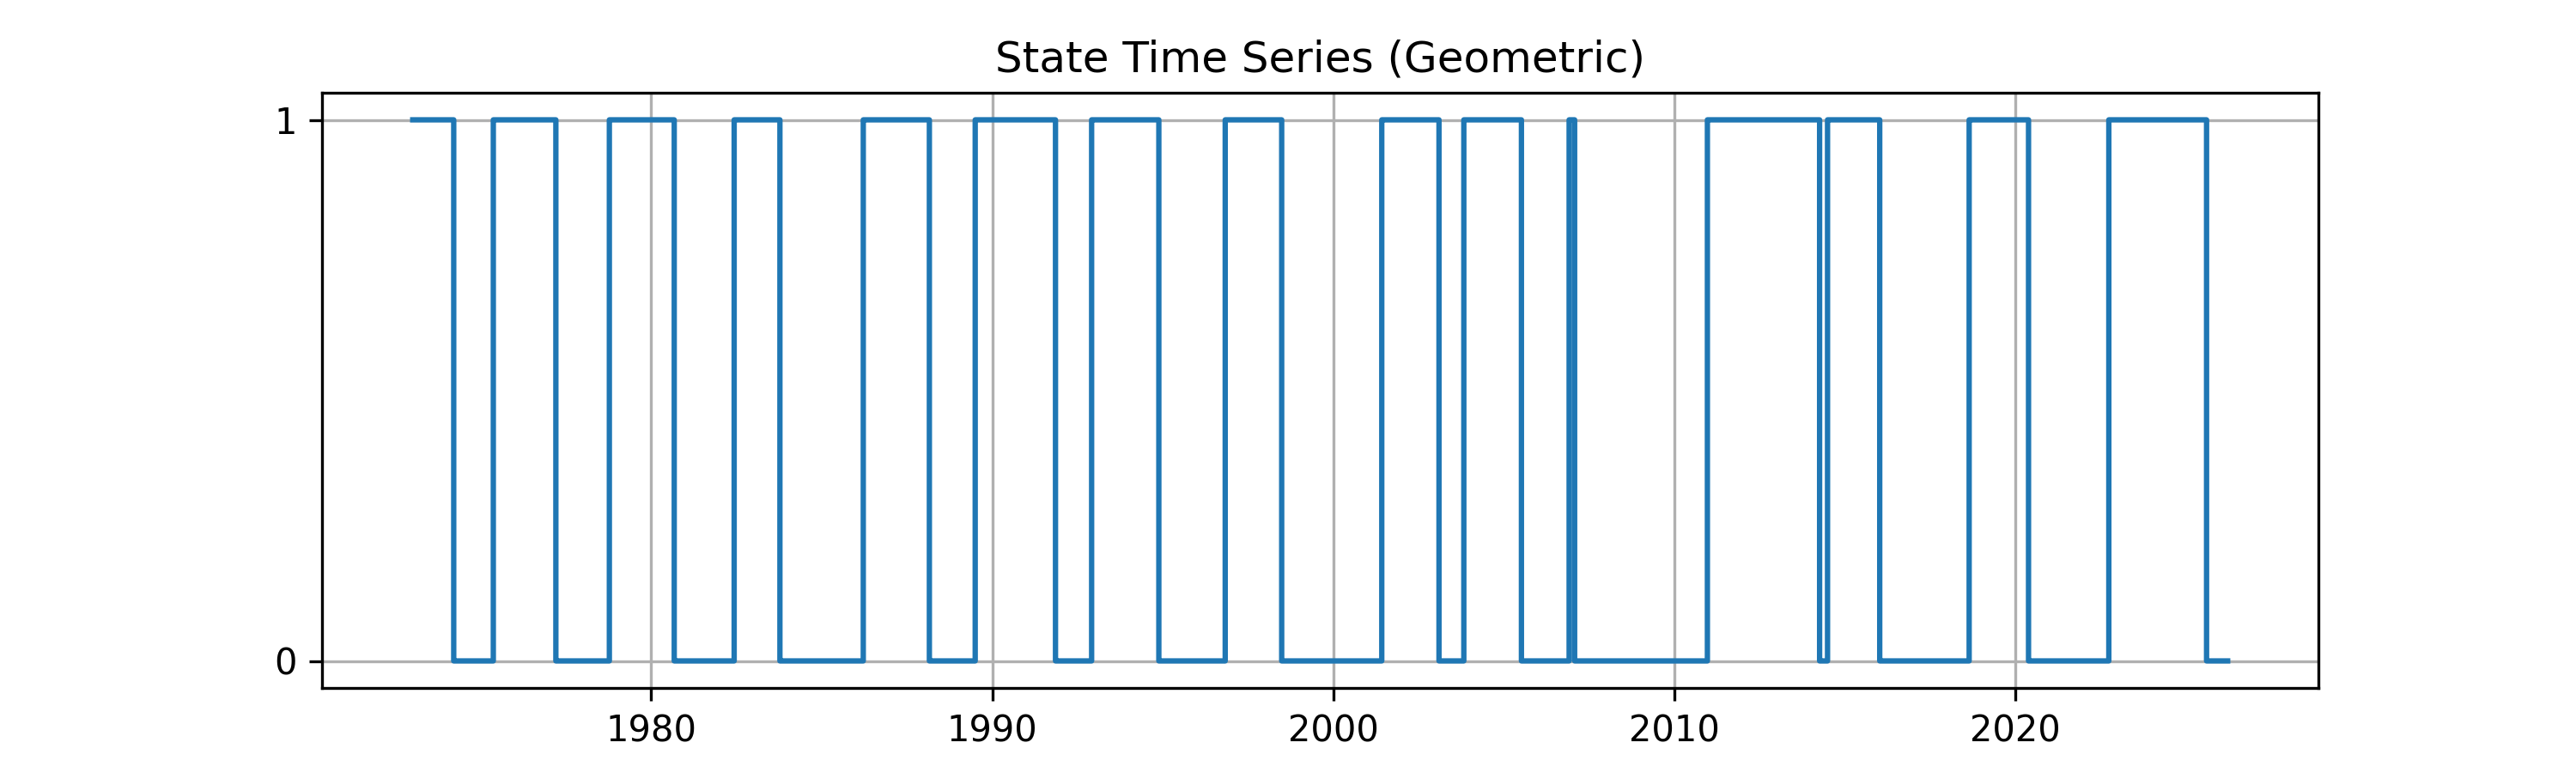
\includegraphics[width=0.5\textwidth]{fig_07_state_timeseries.png}
\caption{Binary state sequence showing transitions between two metastable states.}
\label{fig:state_timeseries}
\end{figure}

The dwell-time distribution (Figure~\ref{fig:dwell_times}) deviates from an exponential form, indicating non-Poisson switching.

\begin{figure}[h!]
\centering
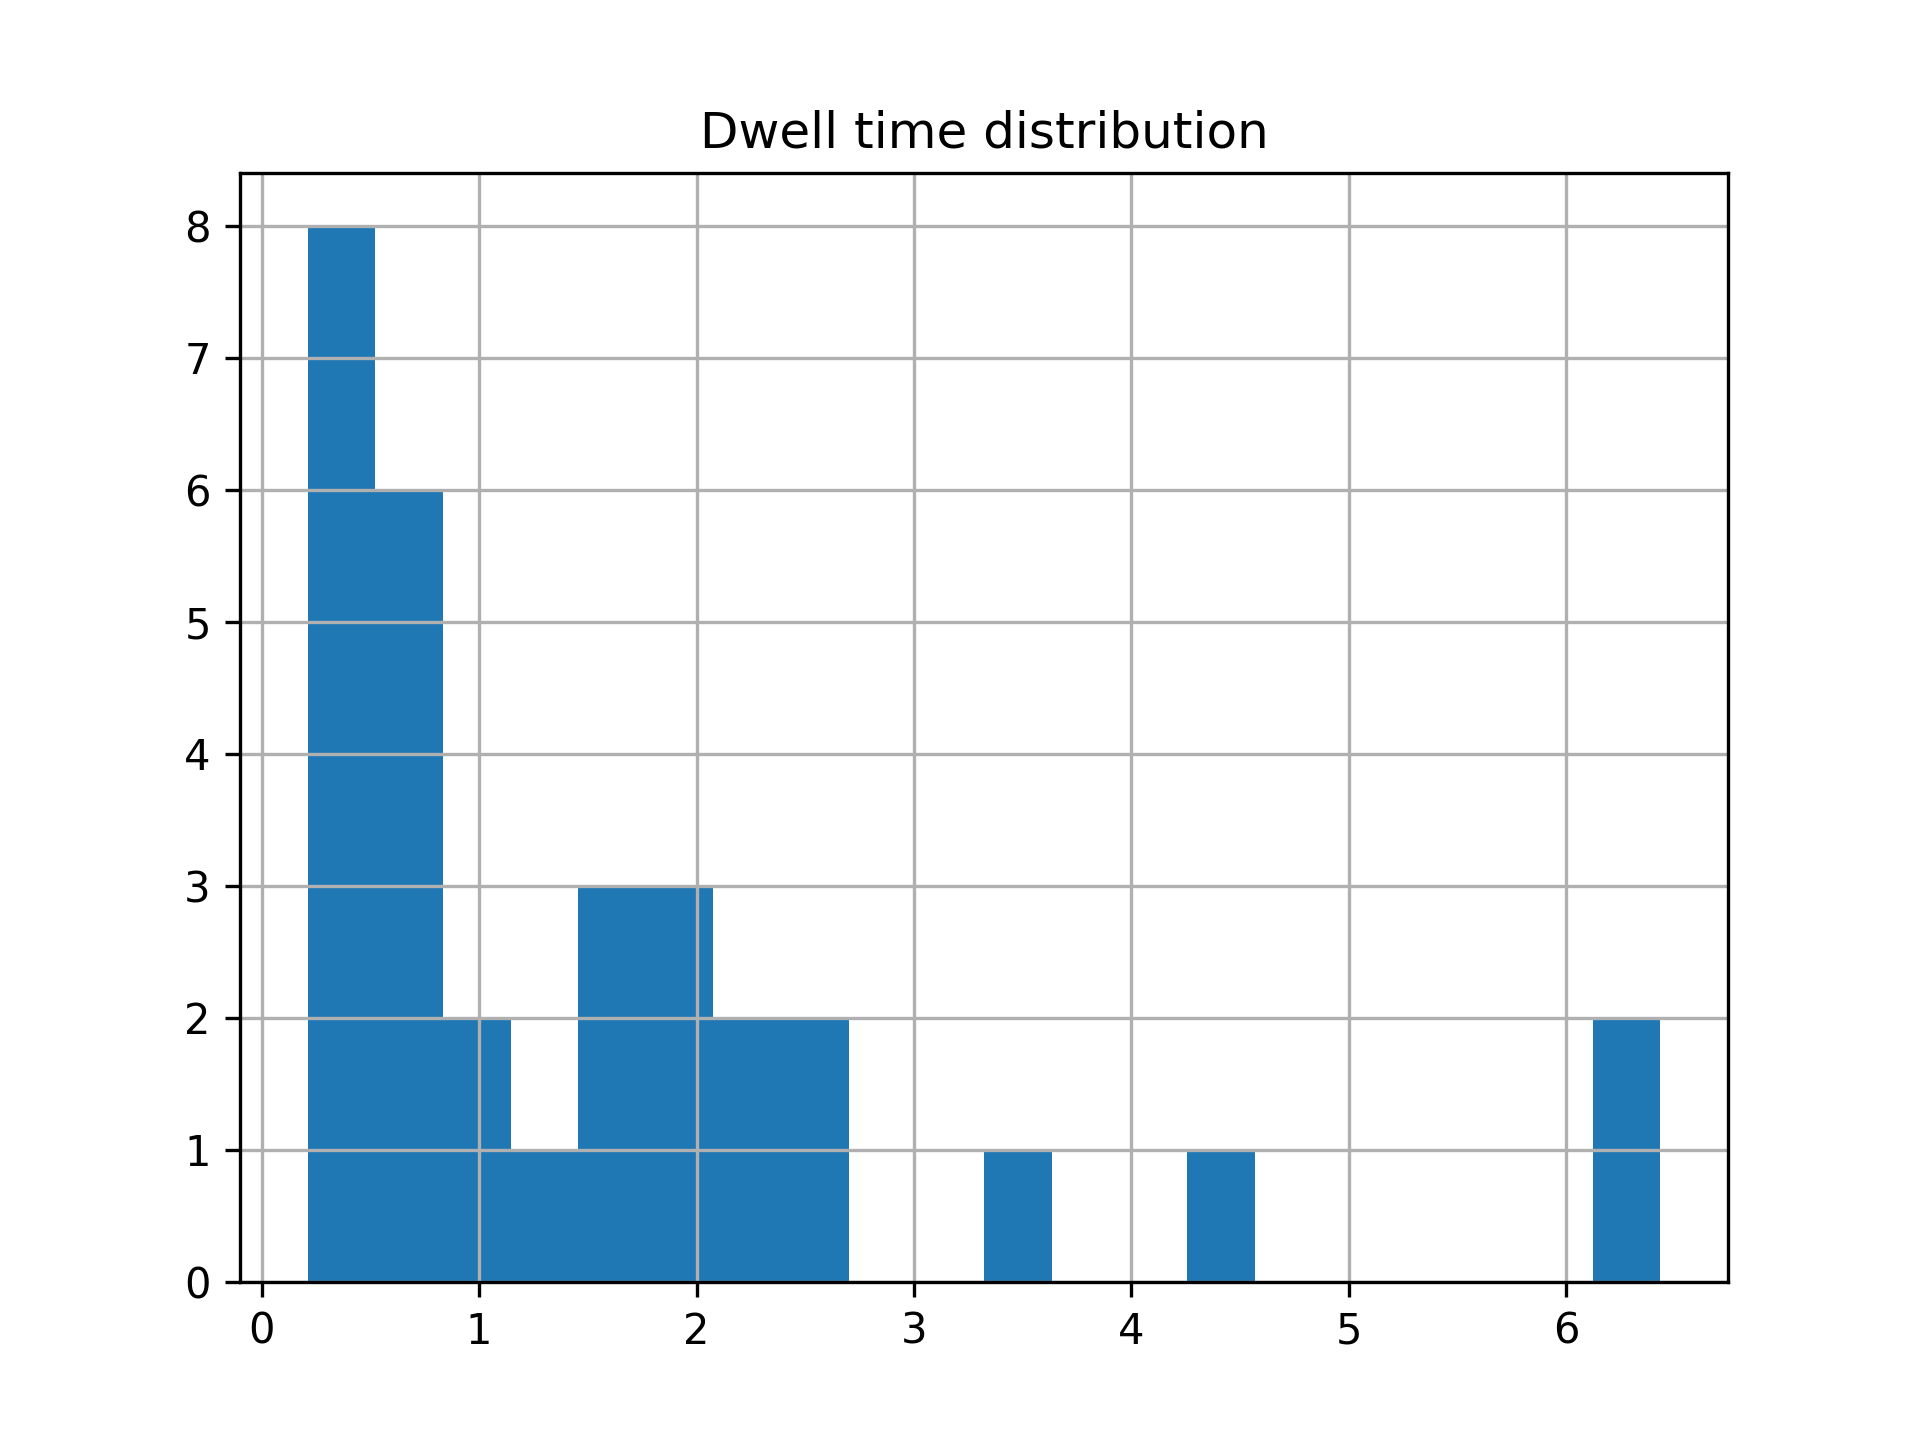
\includegraphics[width=0.5\textwidth]{fig_42_dwell_times.png}
\caption{Distribution of dwell times within each state. Deviation from exponential form indicates structured switching dynamics.}
\label{fig:dwell_times}
\end{figure}

\paragraph{Geometric versus Trivial Bimodality.}
A potential concern is that bimodality may arise trivially from projecting a roughly circular or elliptical trajectory onto a single axis. To address this, we emphasize that the observed two-state structure is not inferred from projection alone, but from the combined evidence of:

\begin{itemize}
\item persistent clustering under multiple independent state definitions (mean, median, and mixture models),
\item non-exponential dwell-time distributions indicating structured, non-Poissonian switching,
\item coherence between state transitions and dynamical indicators such as angular velocity bursts (Section~\ref{subsec:interpretation}).
\end{itemize}

Taken together, these features indicate that the bistable organization reflects temporal structure in the dynamics rather than a purely geometric artifact of projection.

\subsection{Robustness of State Structure}
\label{subsec:robustness_of_state_structure}

The two-state organization is found to be robust under
multiple definitions:

\begin{itemize}
\item Mean threshold
\item Median threshold
\item Gaussian mixture clustering
\end{itemize}

Transition counts and dwell times remain consistent
across all methods, with $\sim 90$ transitions and mean
dwell times of $\sim 200$ time steps.

This demonstrates that the bistable structure is not an
artefact of threshold selection, but an intrinsic feature
of the system.

Beyond simple transition counts, the temporal structure
of switching exhibits clear deviations from memoryless
behavior. The dwell-time distribution (Fig. 7) departs
from an exponential form, indicating non-Poissonian
dynamics and suggesting the presence of state-dependent
persistence.

This observation is reinforced by later analysis of the
angular velocity (Section~\ref{subsec:interpretation}), where transitions appear
as burst-like events embedded within longer intervals of
coherent evolution. Together, these results indicate that
state switching is not purely stochastic, but reflects
structured intermittency within the system’s dynamics.

\section{Residual Phase-Space Structure and Spectral Content}
\label{sec:residual_phase}

To isolate the intrinsic dynamics of polar motion, we examine the residual trajectory after removal of dominant deterministic components. The resulting motion is analyzed directly in $(x_{\mathrm{res}}, y_{\mathrm{res}})$ phase space, preserving geometric relationships without projection or dimensional reduction.

\subsection{Residual Phase-Space Trajectory}
\label{subsec:residual_phase_space_trajectory}

\begin{figure}[h!]
\centering
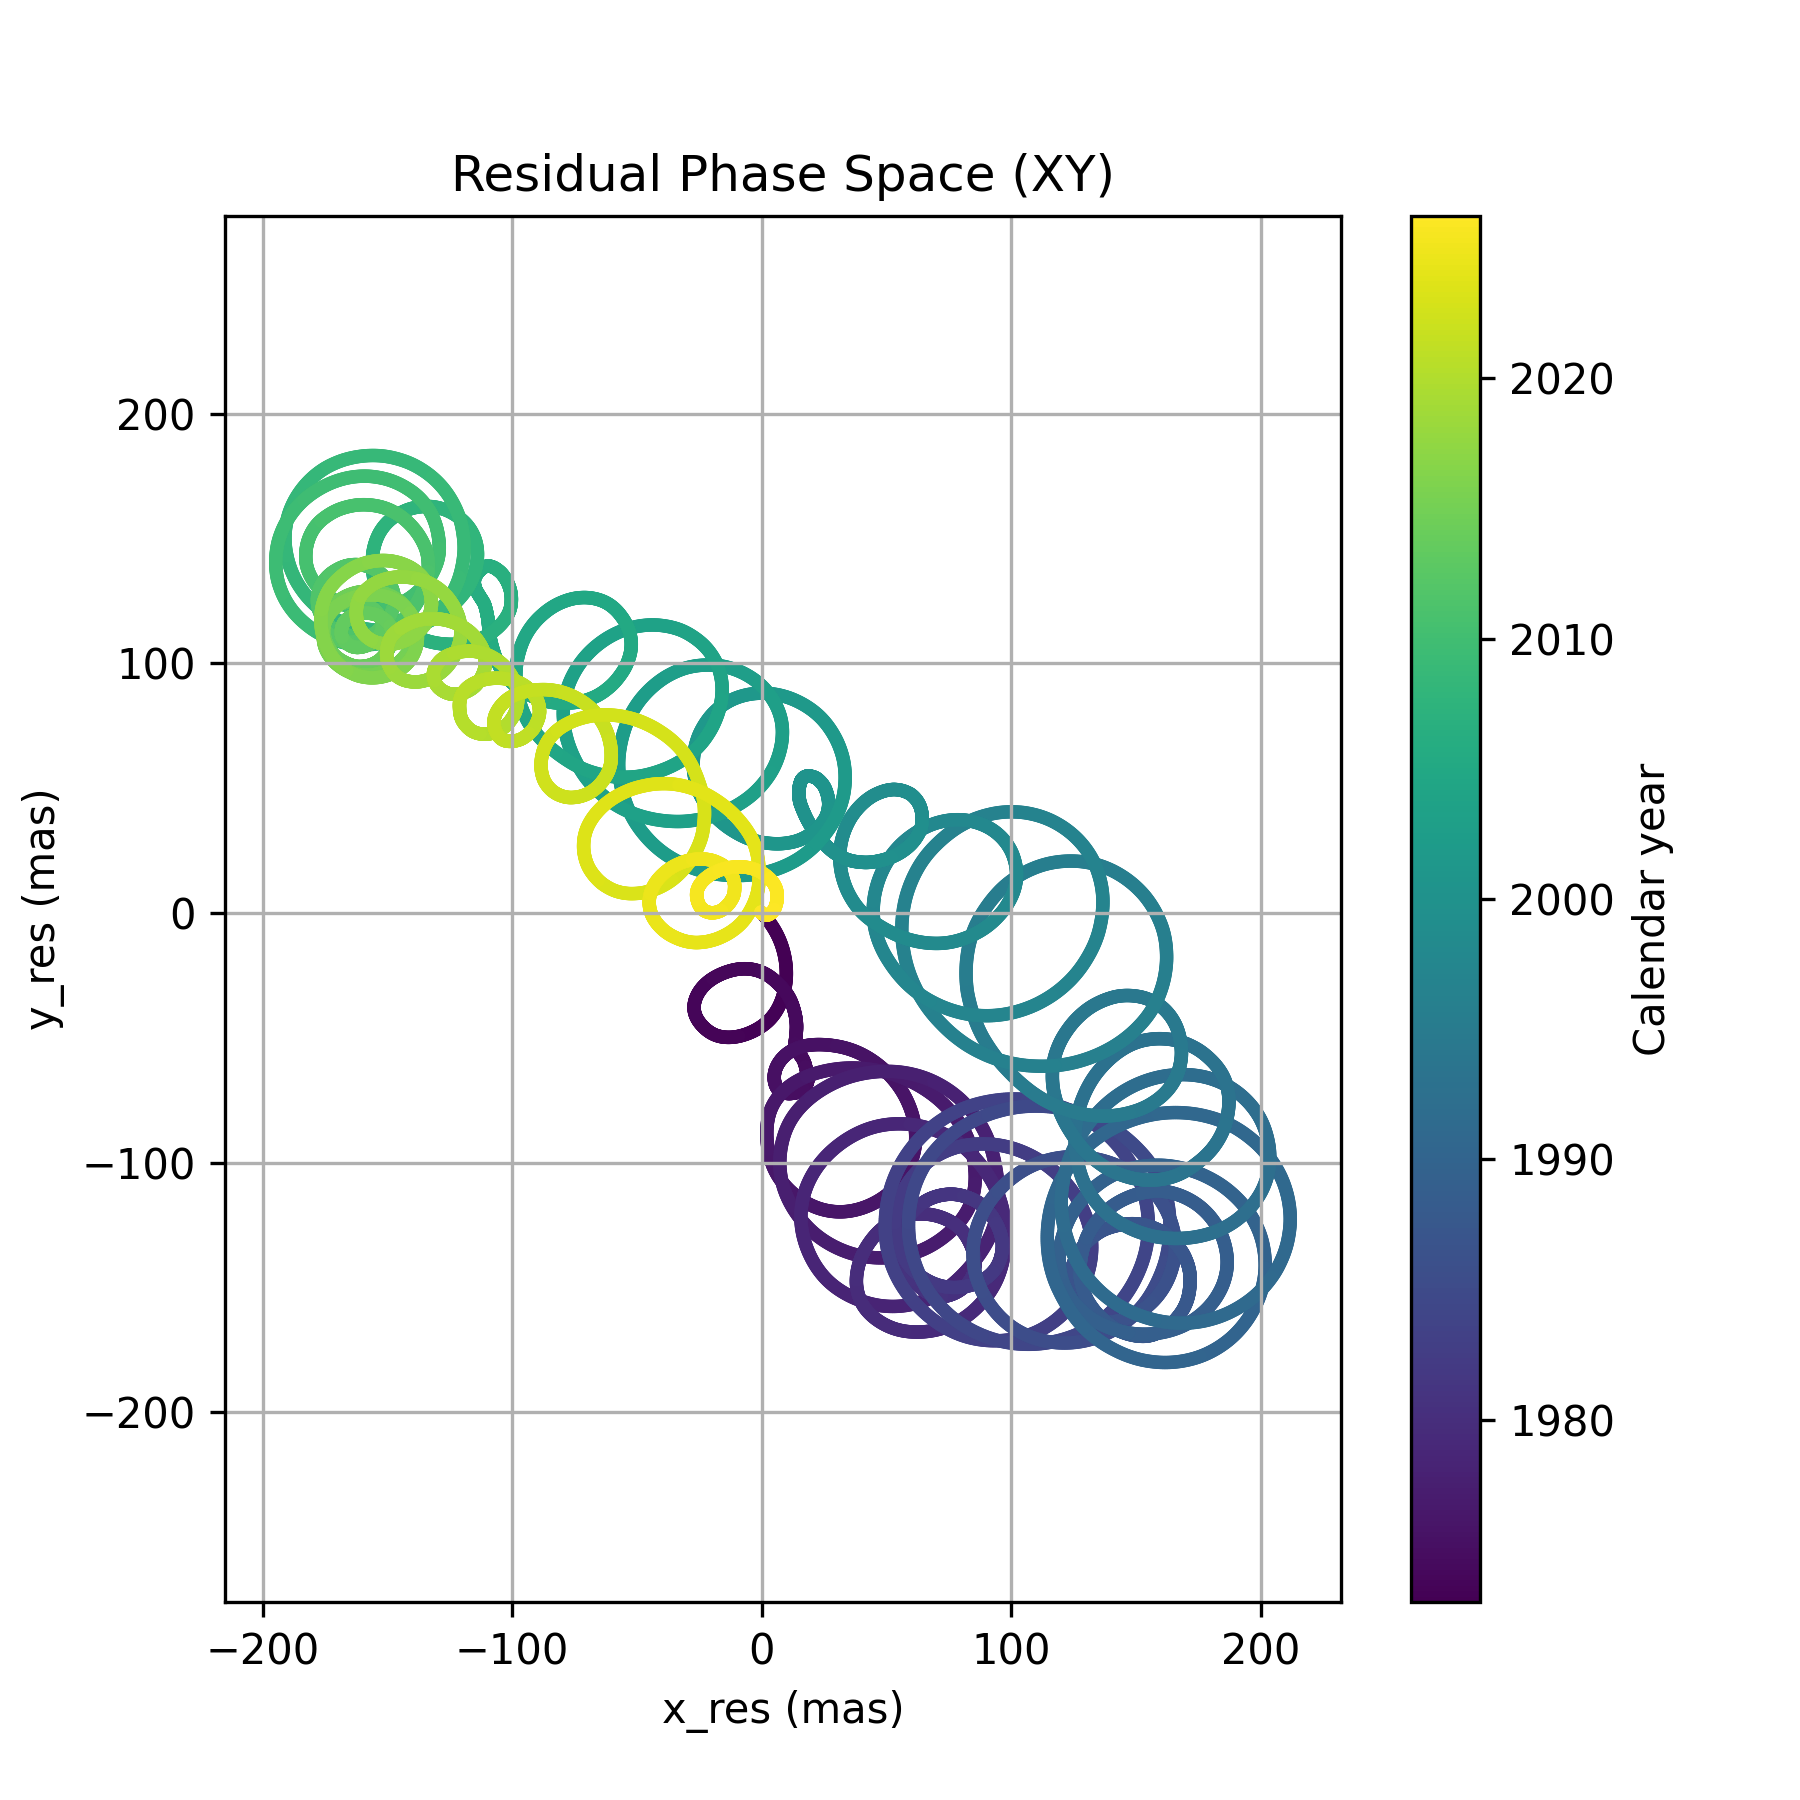
\includegraphics[width=0.5\textwidth]{fig_12a_residual_path.png}
\caption{
Residual polar motion trajectory in $(x_{\mathrm{res}}, y_{\mathrm{res}})$ space, colored by calendar year. The trajectory exhibits a sequence of looping structures embedded within a larger-scale drift. The persistence and coherence of these loops suggest a quasi-periodic component superimposed on a slower translational mode.
}
\end{figure}

The residual trajectory reveals a structured path consisting of repeated loops rather than stochastic dispersion. The approximate count and spacing of these loops are consistent with a sub-annual to interannual oscillatory component, embedded within a longer-timescale drift.

\subsection{Drift Structure and Preferred Axis}
\label{subsec:drift_structure_and_preferred_axis}

\begin{figure}[h!]
\centering
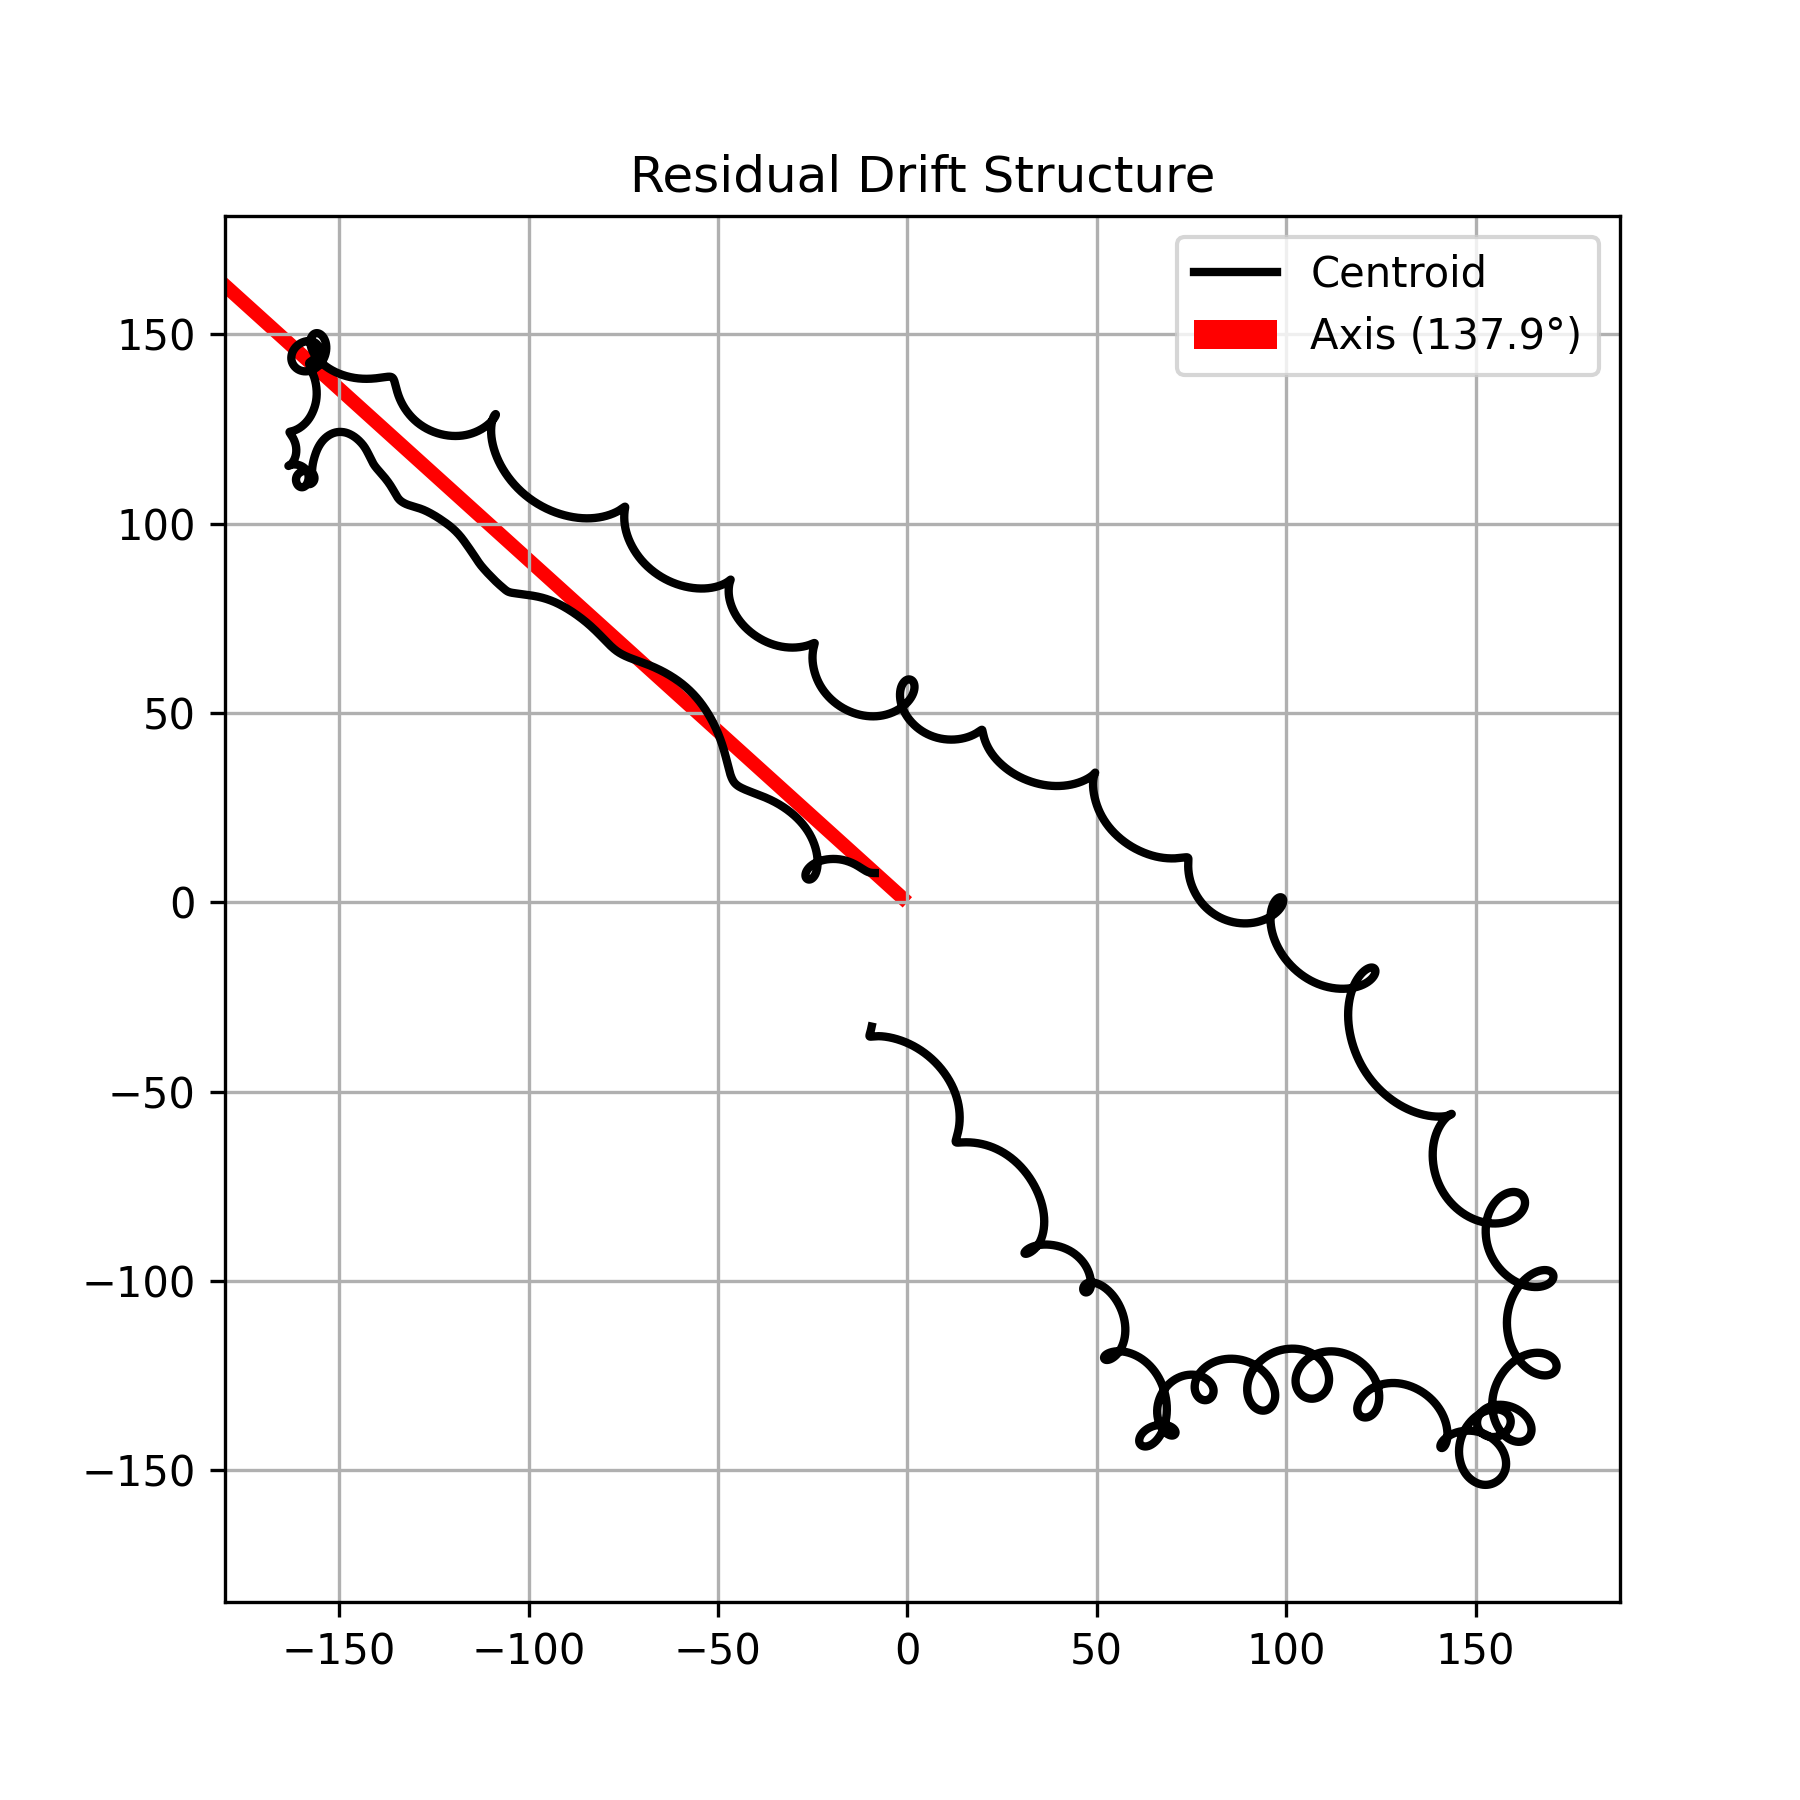
\includegraphics[width=0.5\textwidth]{fig_12b_residual_structure.png}
\caption{
Centroid trajectory of the residual motion (black) with best-fit linear drift axis (red). The motion organizes along a well-defined orientation, indicating anisotropic structure in the residual phase space. The centroid path traces a smooth progression, while local looping behavior persists around this axis.
}
\end{figure}

The residual motion is not isotropic. Instead, it exhibits a clear preferred orientation, with the centroid trajectory aligning along a stable axis. This indicates that the residual dynamics are governed by a constrained geometry, rather than random fluctuations.

\subsection{Combined Phase-Space Representation}
\label{subsec:combined_phase_space_representation}

\begin{figure}[h!]
\centering
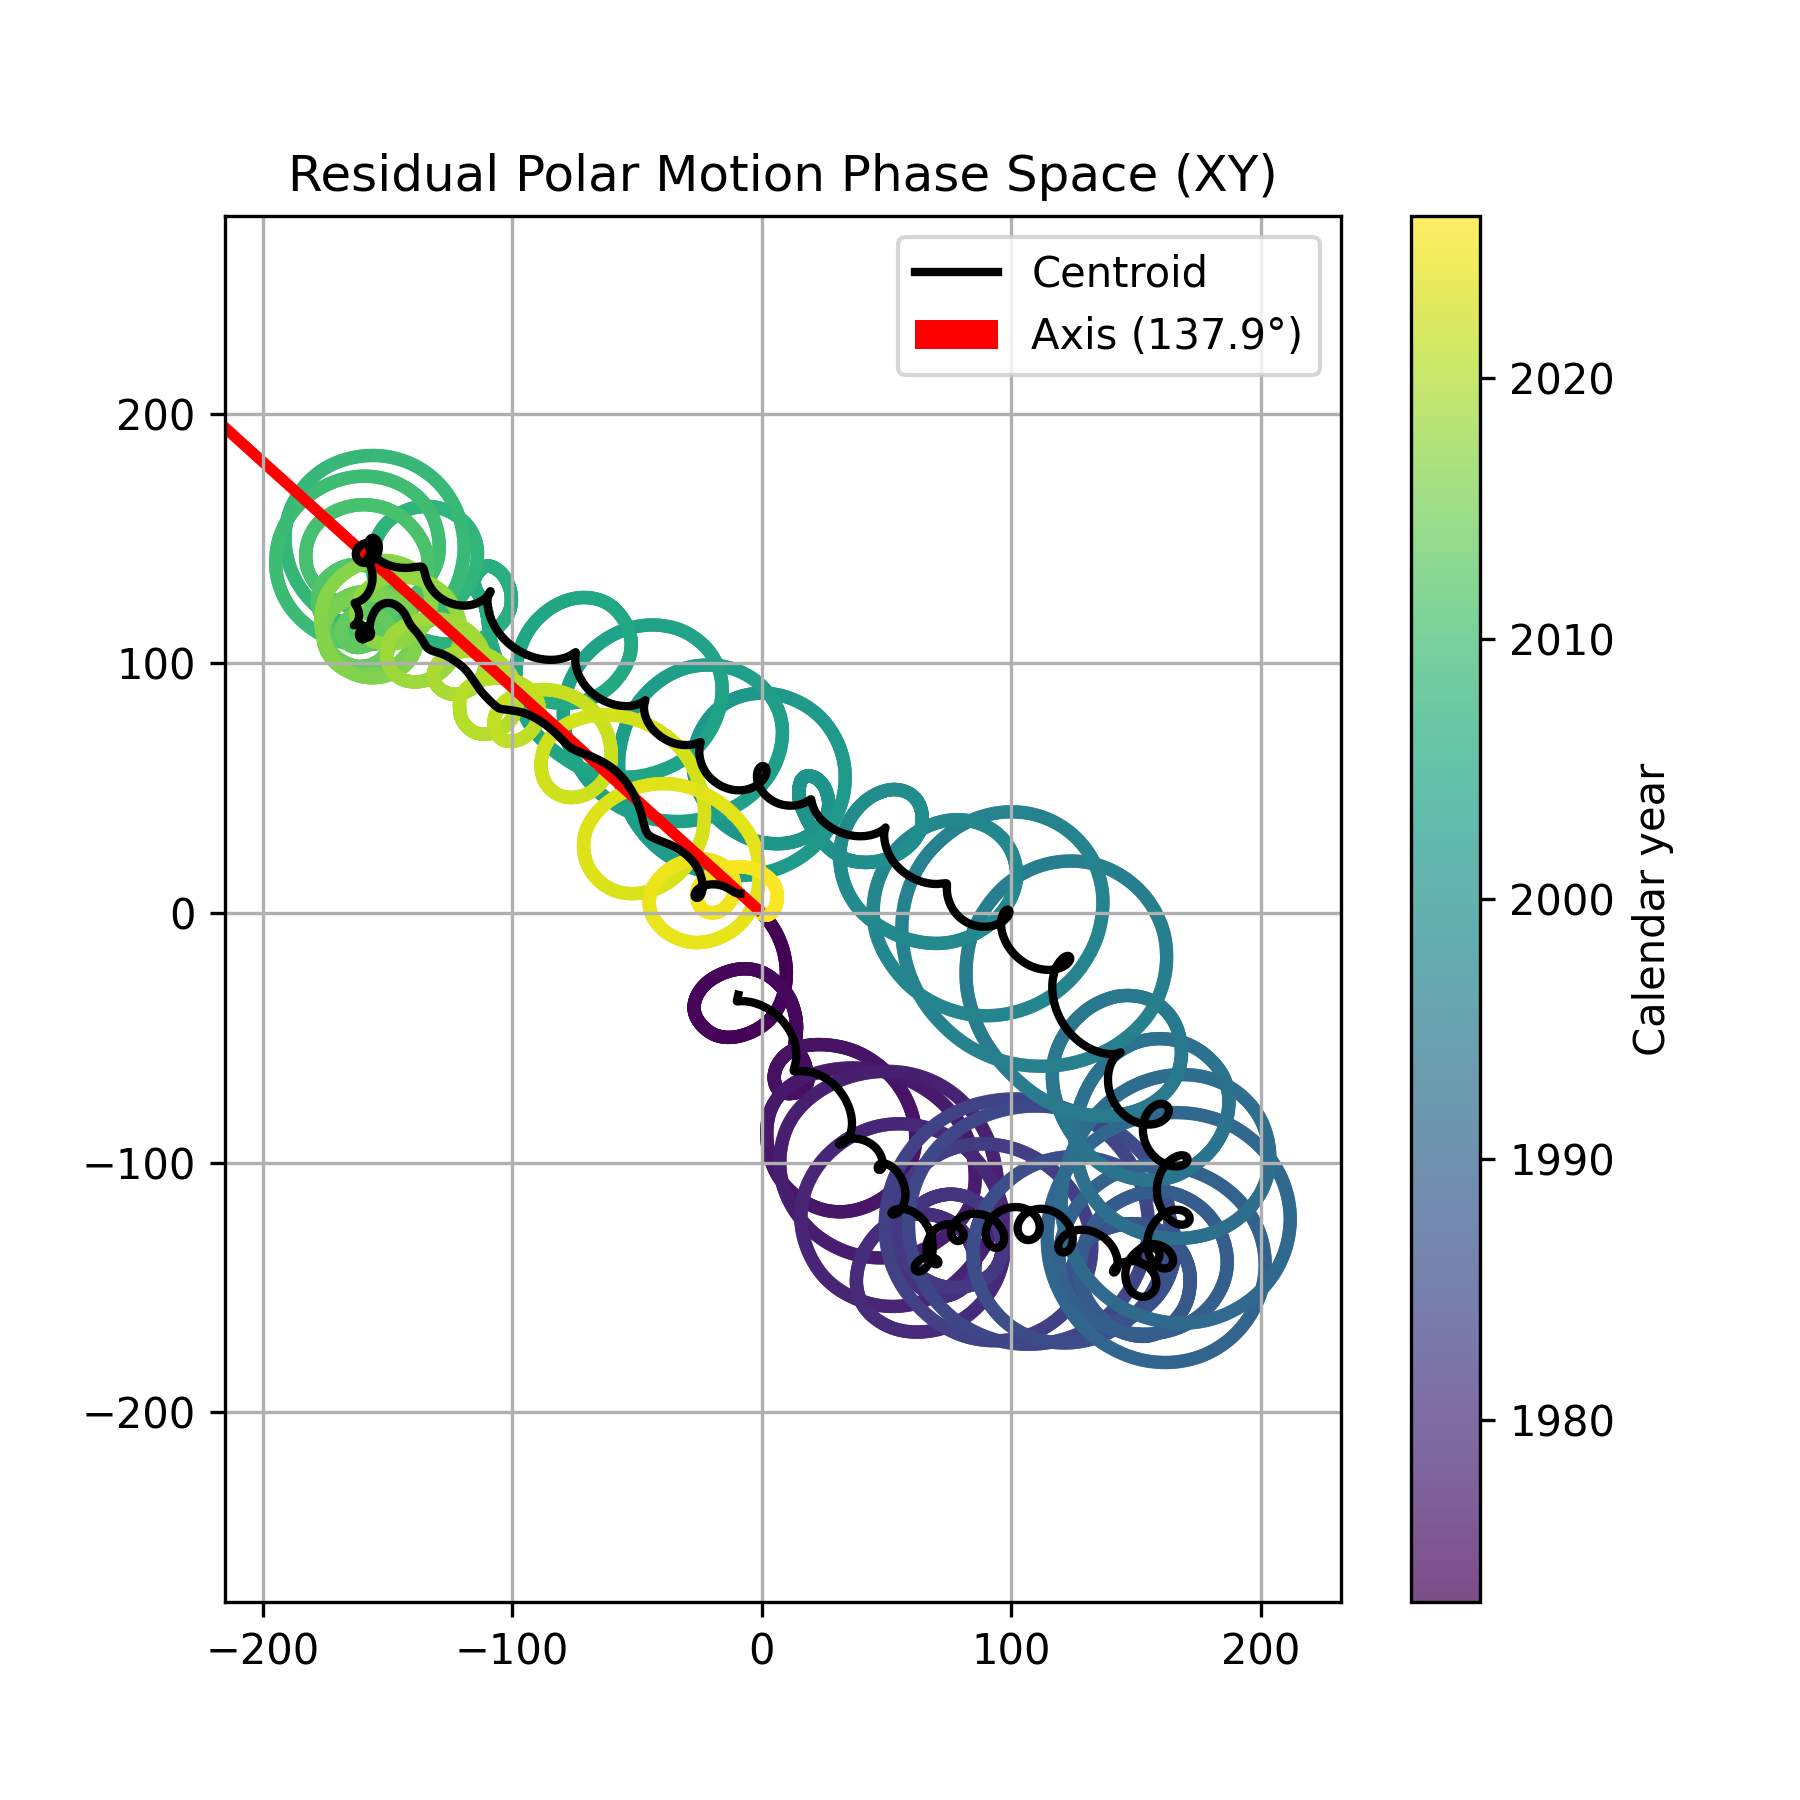
\includegraphics[width=0.5\textwidth]{fig_12c_residual_combined.png}
\caption{
Combined view of residual phase-space trajectory and drift structure. The looping motion remains phase-locked to the underlying drift axis, indicating a superposition of oscillatory and translational modes. Temporal coloring shows continuity of evolution rather than discrete regime transitions.
}
\end{figure}

When viewed together, the structure resolves into a coherent dynamical pattern: a looping trajectory that advances along a fixed axis. This behavior is consistent with a weakly coupled system in which an oscillatory mode is advected by a slower drift.

\subsection{Spectral Signature of Residual Motion}
\label{subsec:spectral_signature_of_residual_motion}

\begin{figure}[h!]
\centering
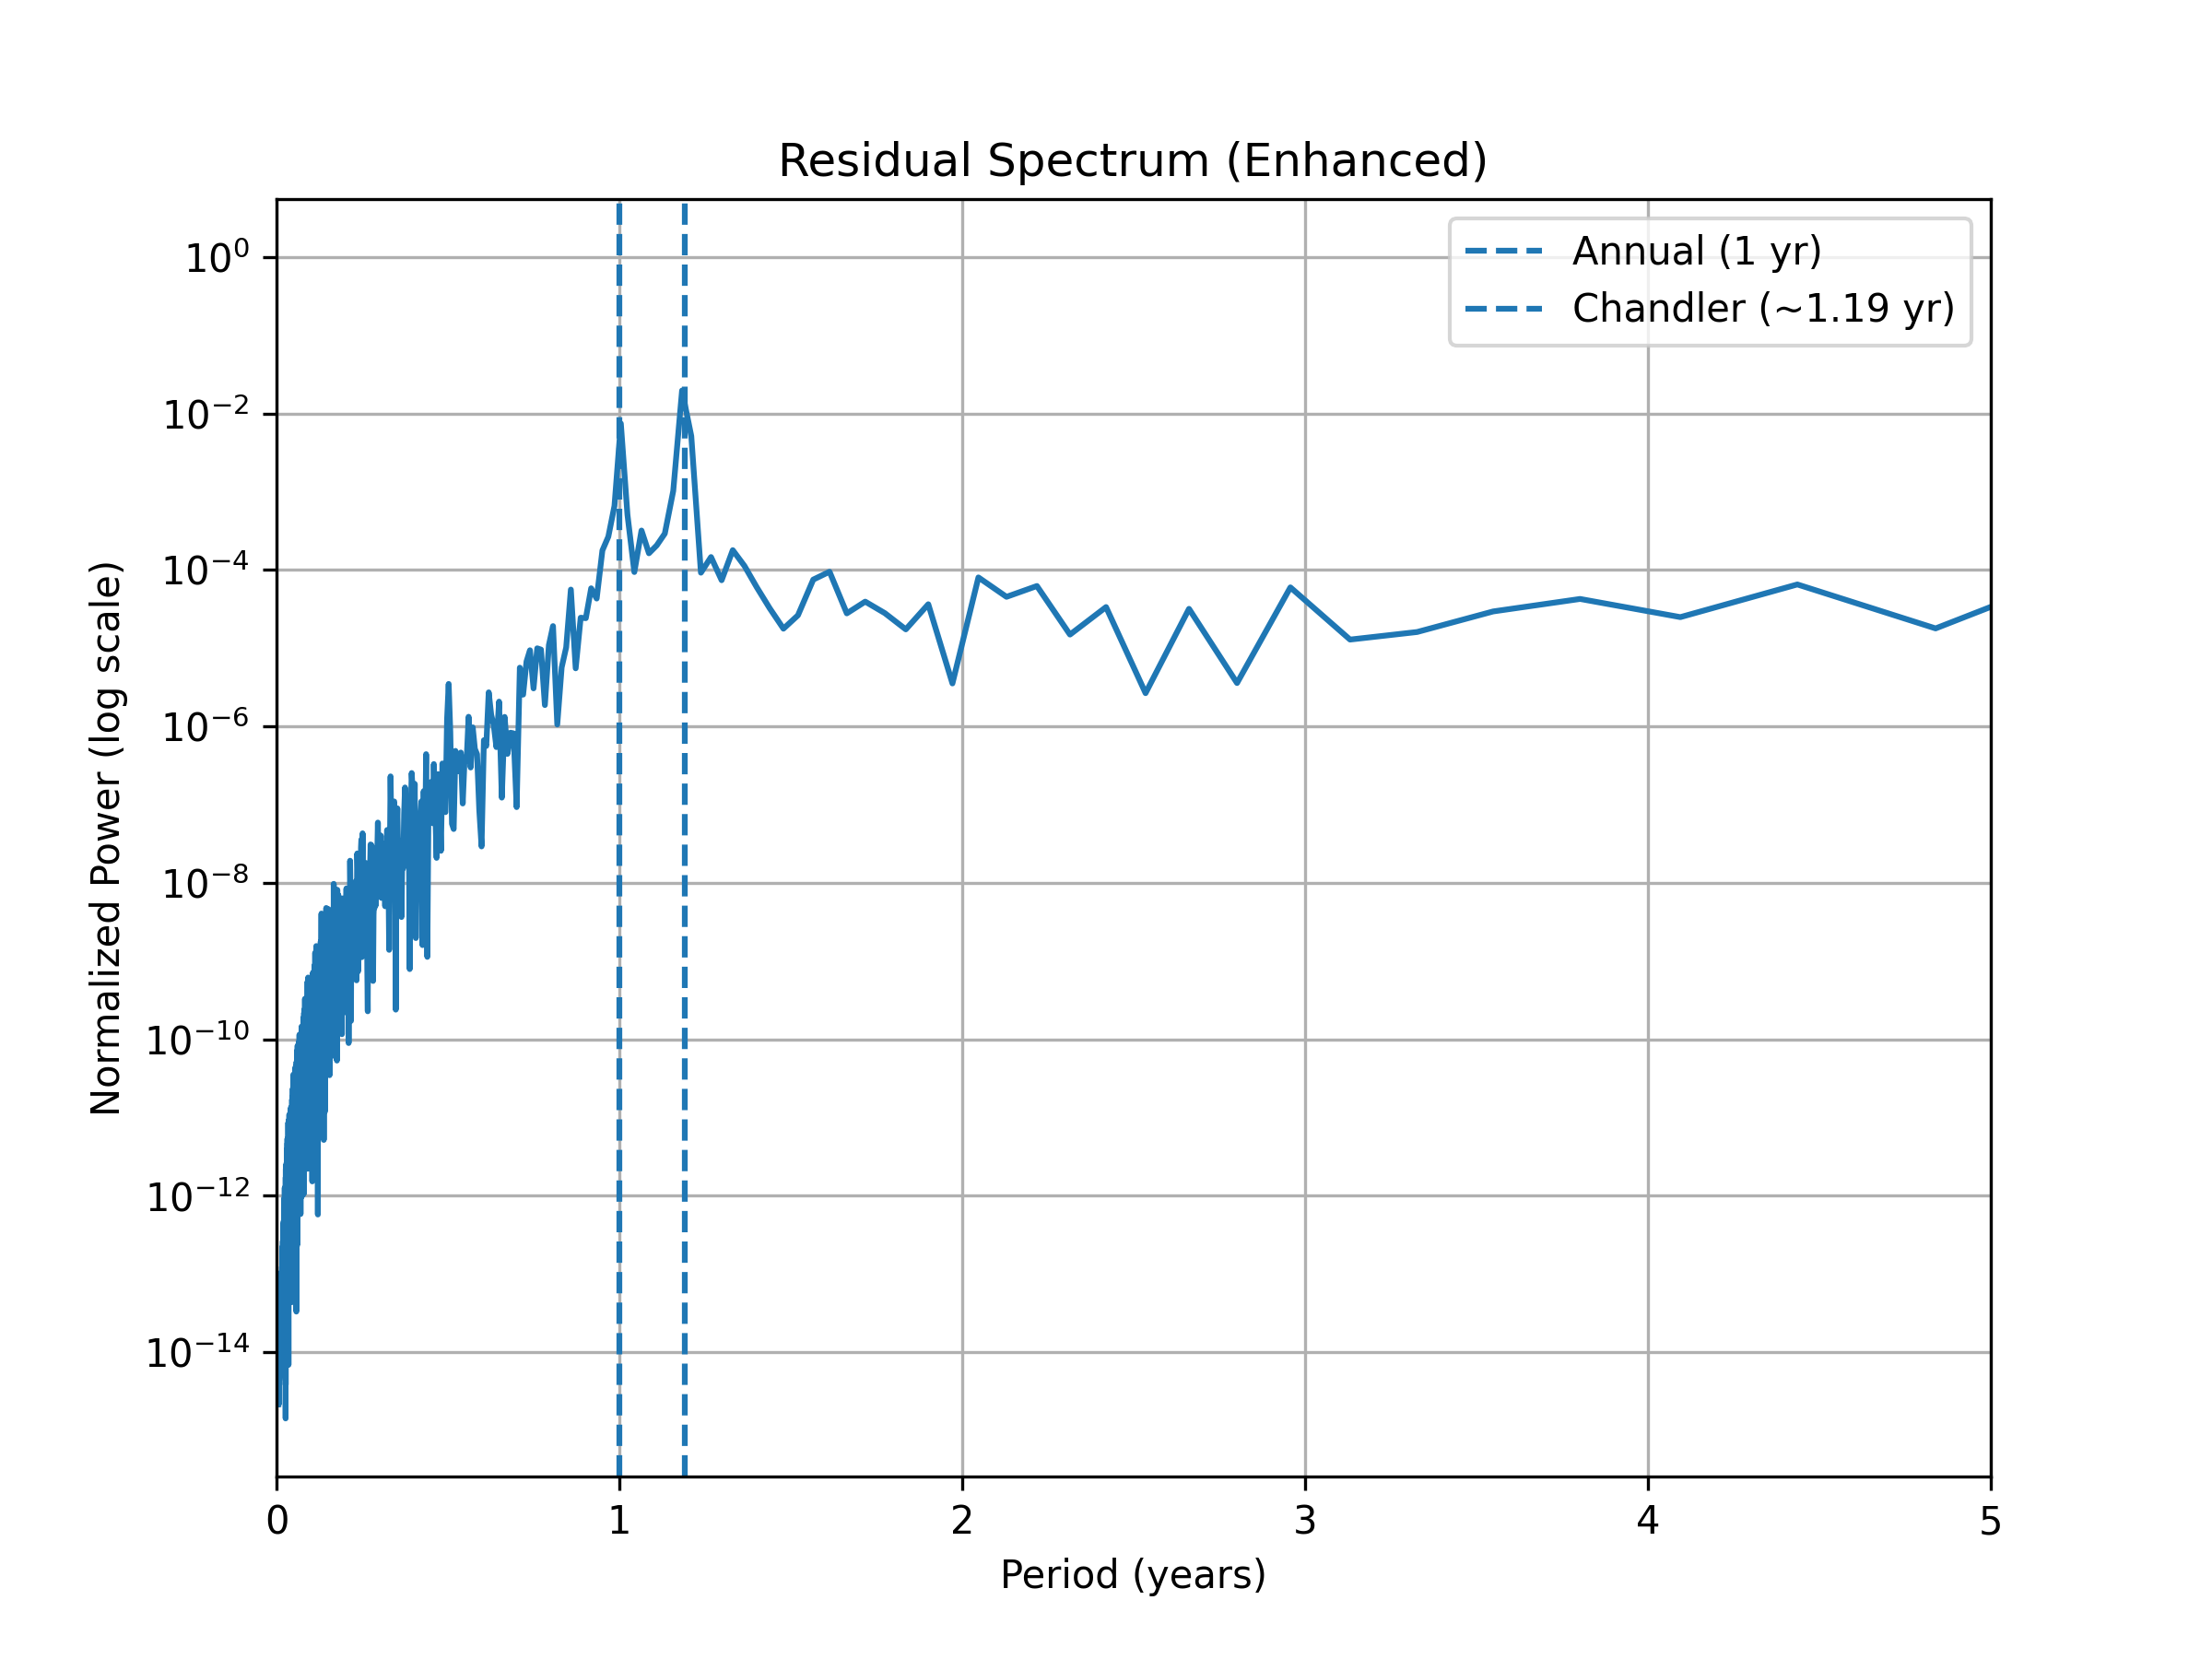
\includegraphics[width=0.5\textwidth]{fig_13_residual_spectrum.png}
\caption{
Enhanced residual power spectrum (log-scaled), normalized for visibility. Two prominent peaks appear near 1.0 year and $\sim$1.2 years, corresponding to annual and Chandler-band periodicities. The logarithmic scaling reveals a broad background structure beyond the dominant peaks.
}
\end{figure}

\begin{figure}[h!]
\centering
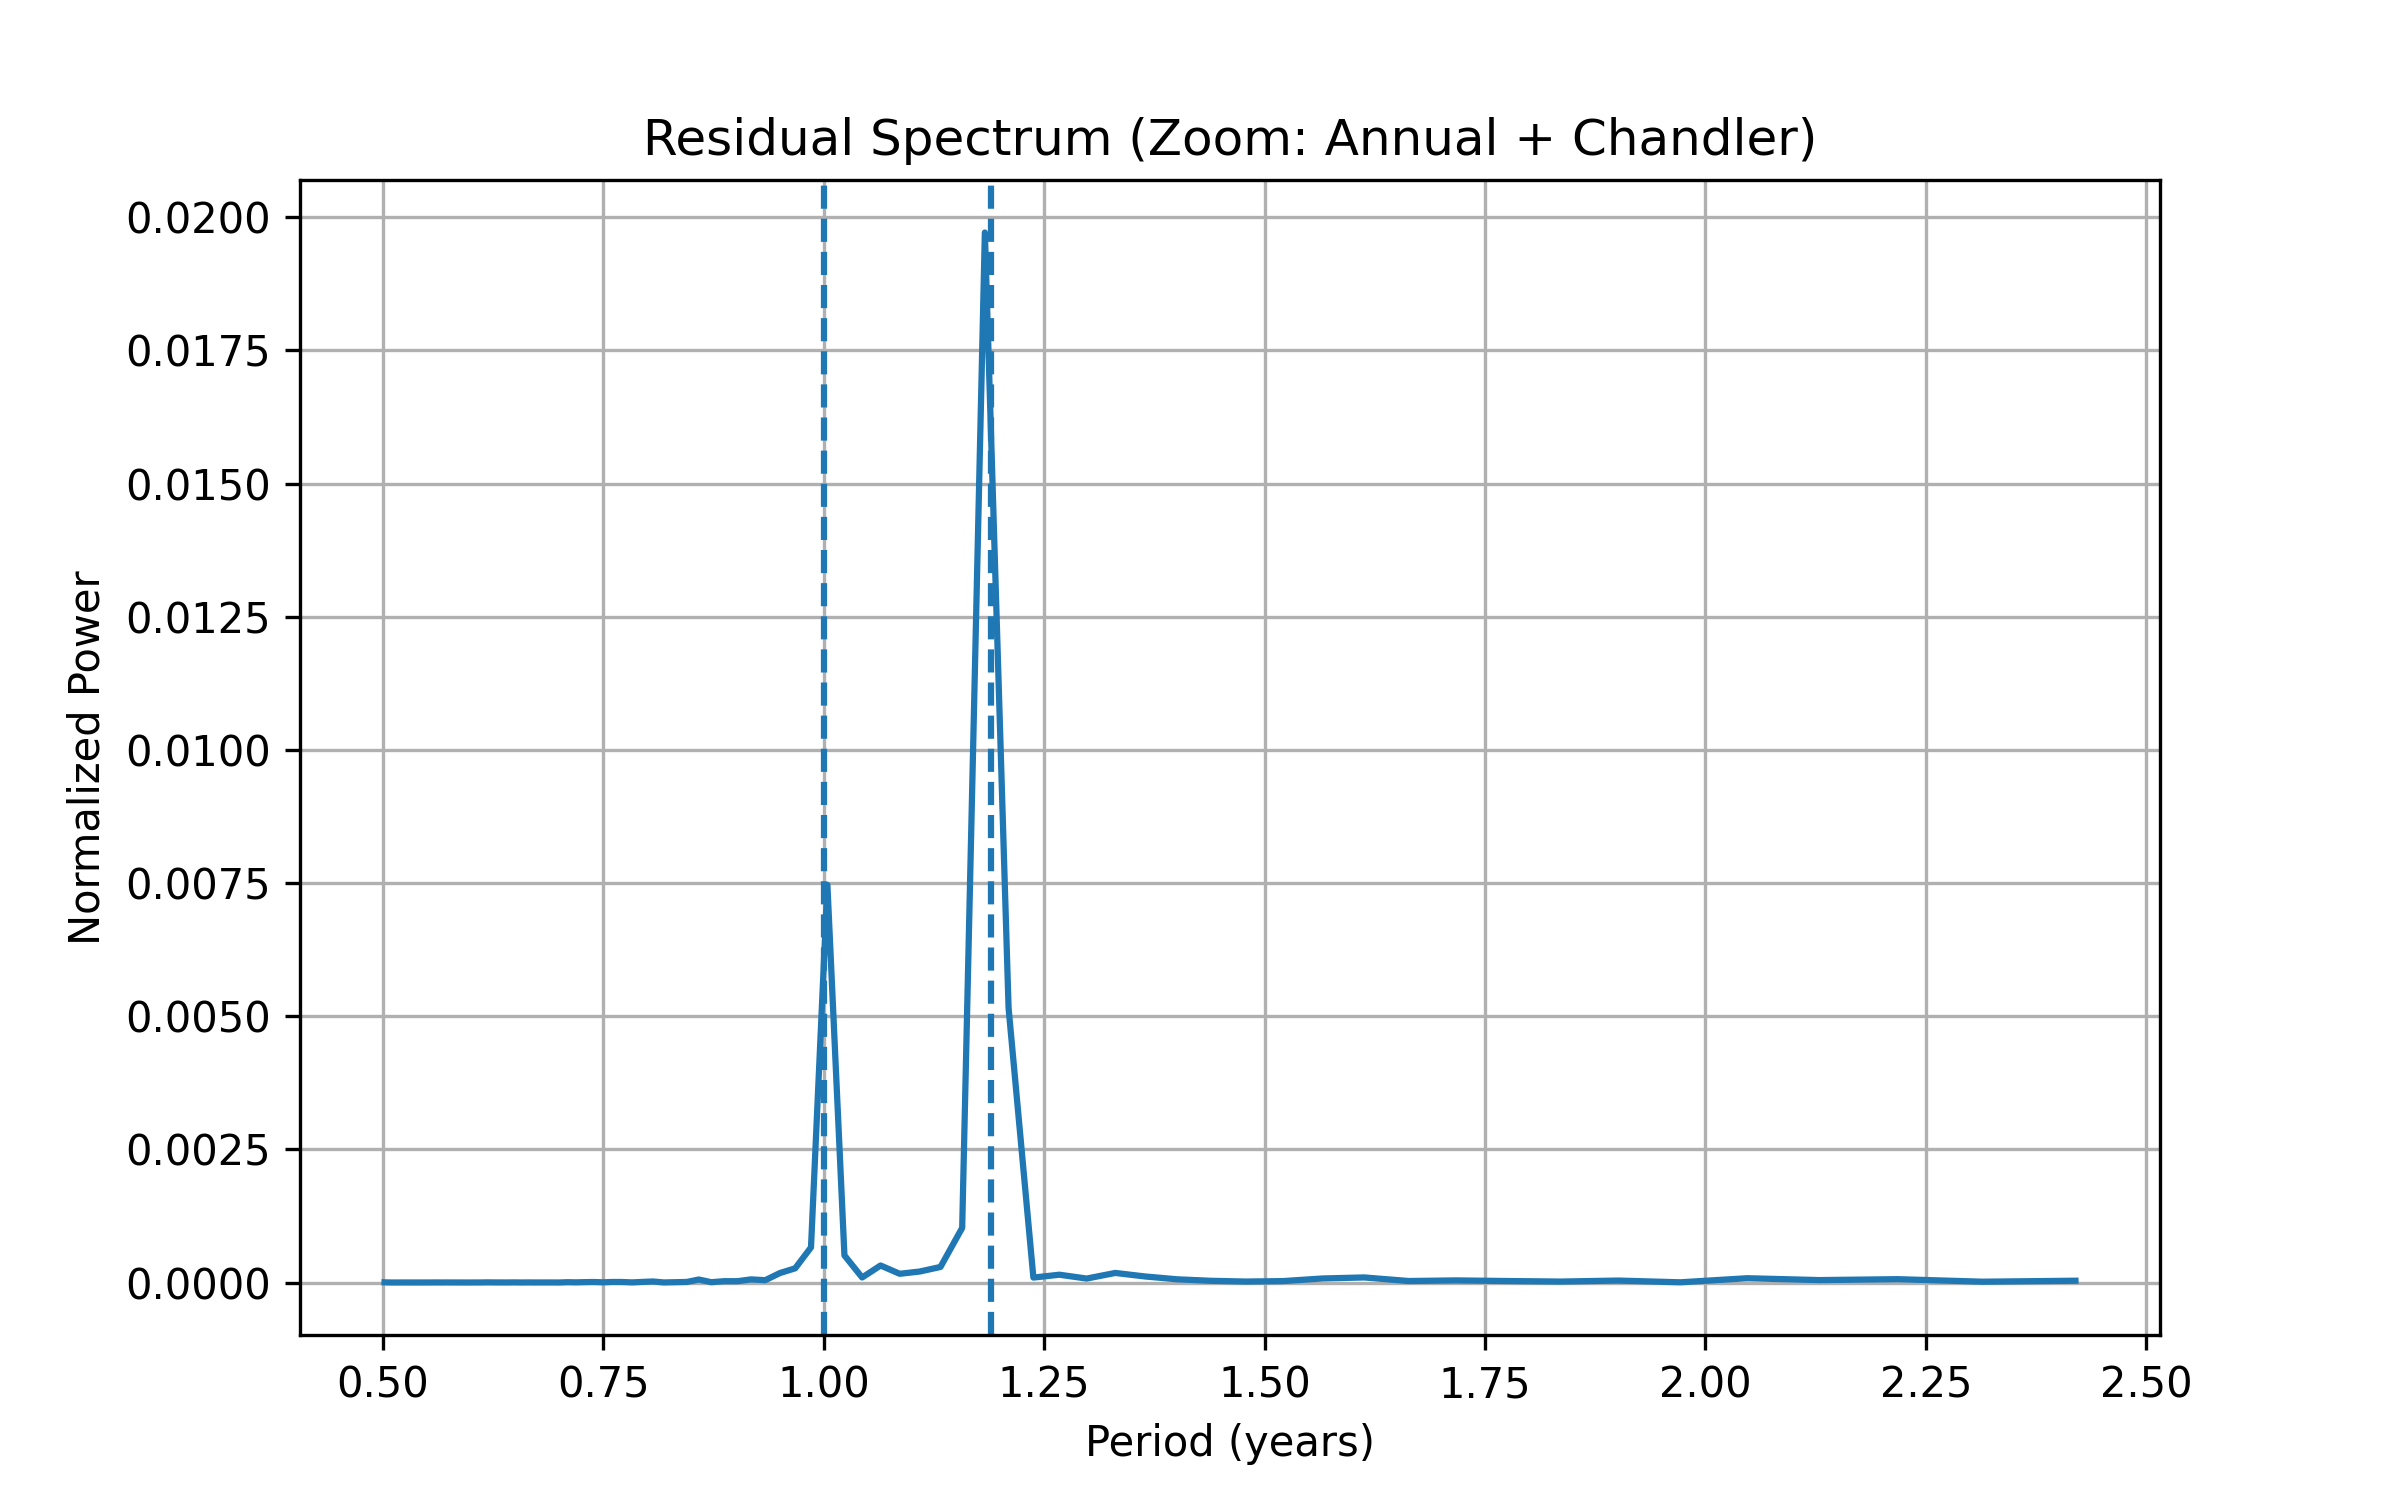
\includegraphics[width=0.5\textwidth]{fig_13b_residual_spectrum_zoom.png}
\caption{
Zoomed spectral view (0.5--2.5 years). The separation between the annual ($\sim$1 year) and Chandler-band ($\sim$1.2 year) peaks is clearly resolved. The Chandler-band peak aligns with the looping structures observed in phase space.
}
\end{figure}

The spectral analysis confirms that the residual motion contains a dominant periodic component in the Chandler band, alongside a smaller annual contribution. Importantly, the phase-space representation shows that this periodicity is not isolated, but embedded within a larger geometric structure.

\subsection{Phase-Space Density and Principal Axes}
\label{subsec:phase_space_density_and_principal_axes}

\begin{figure}[h!]
\centering
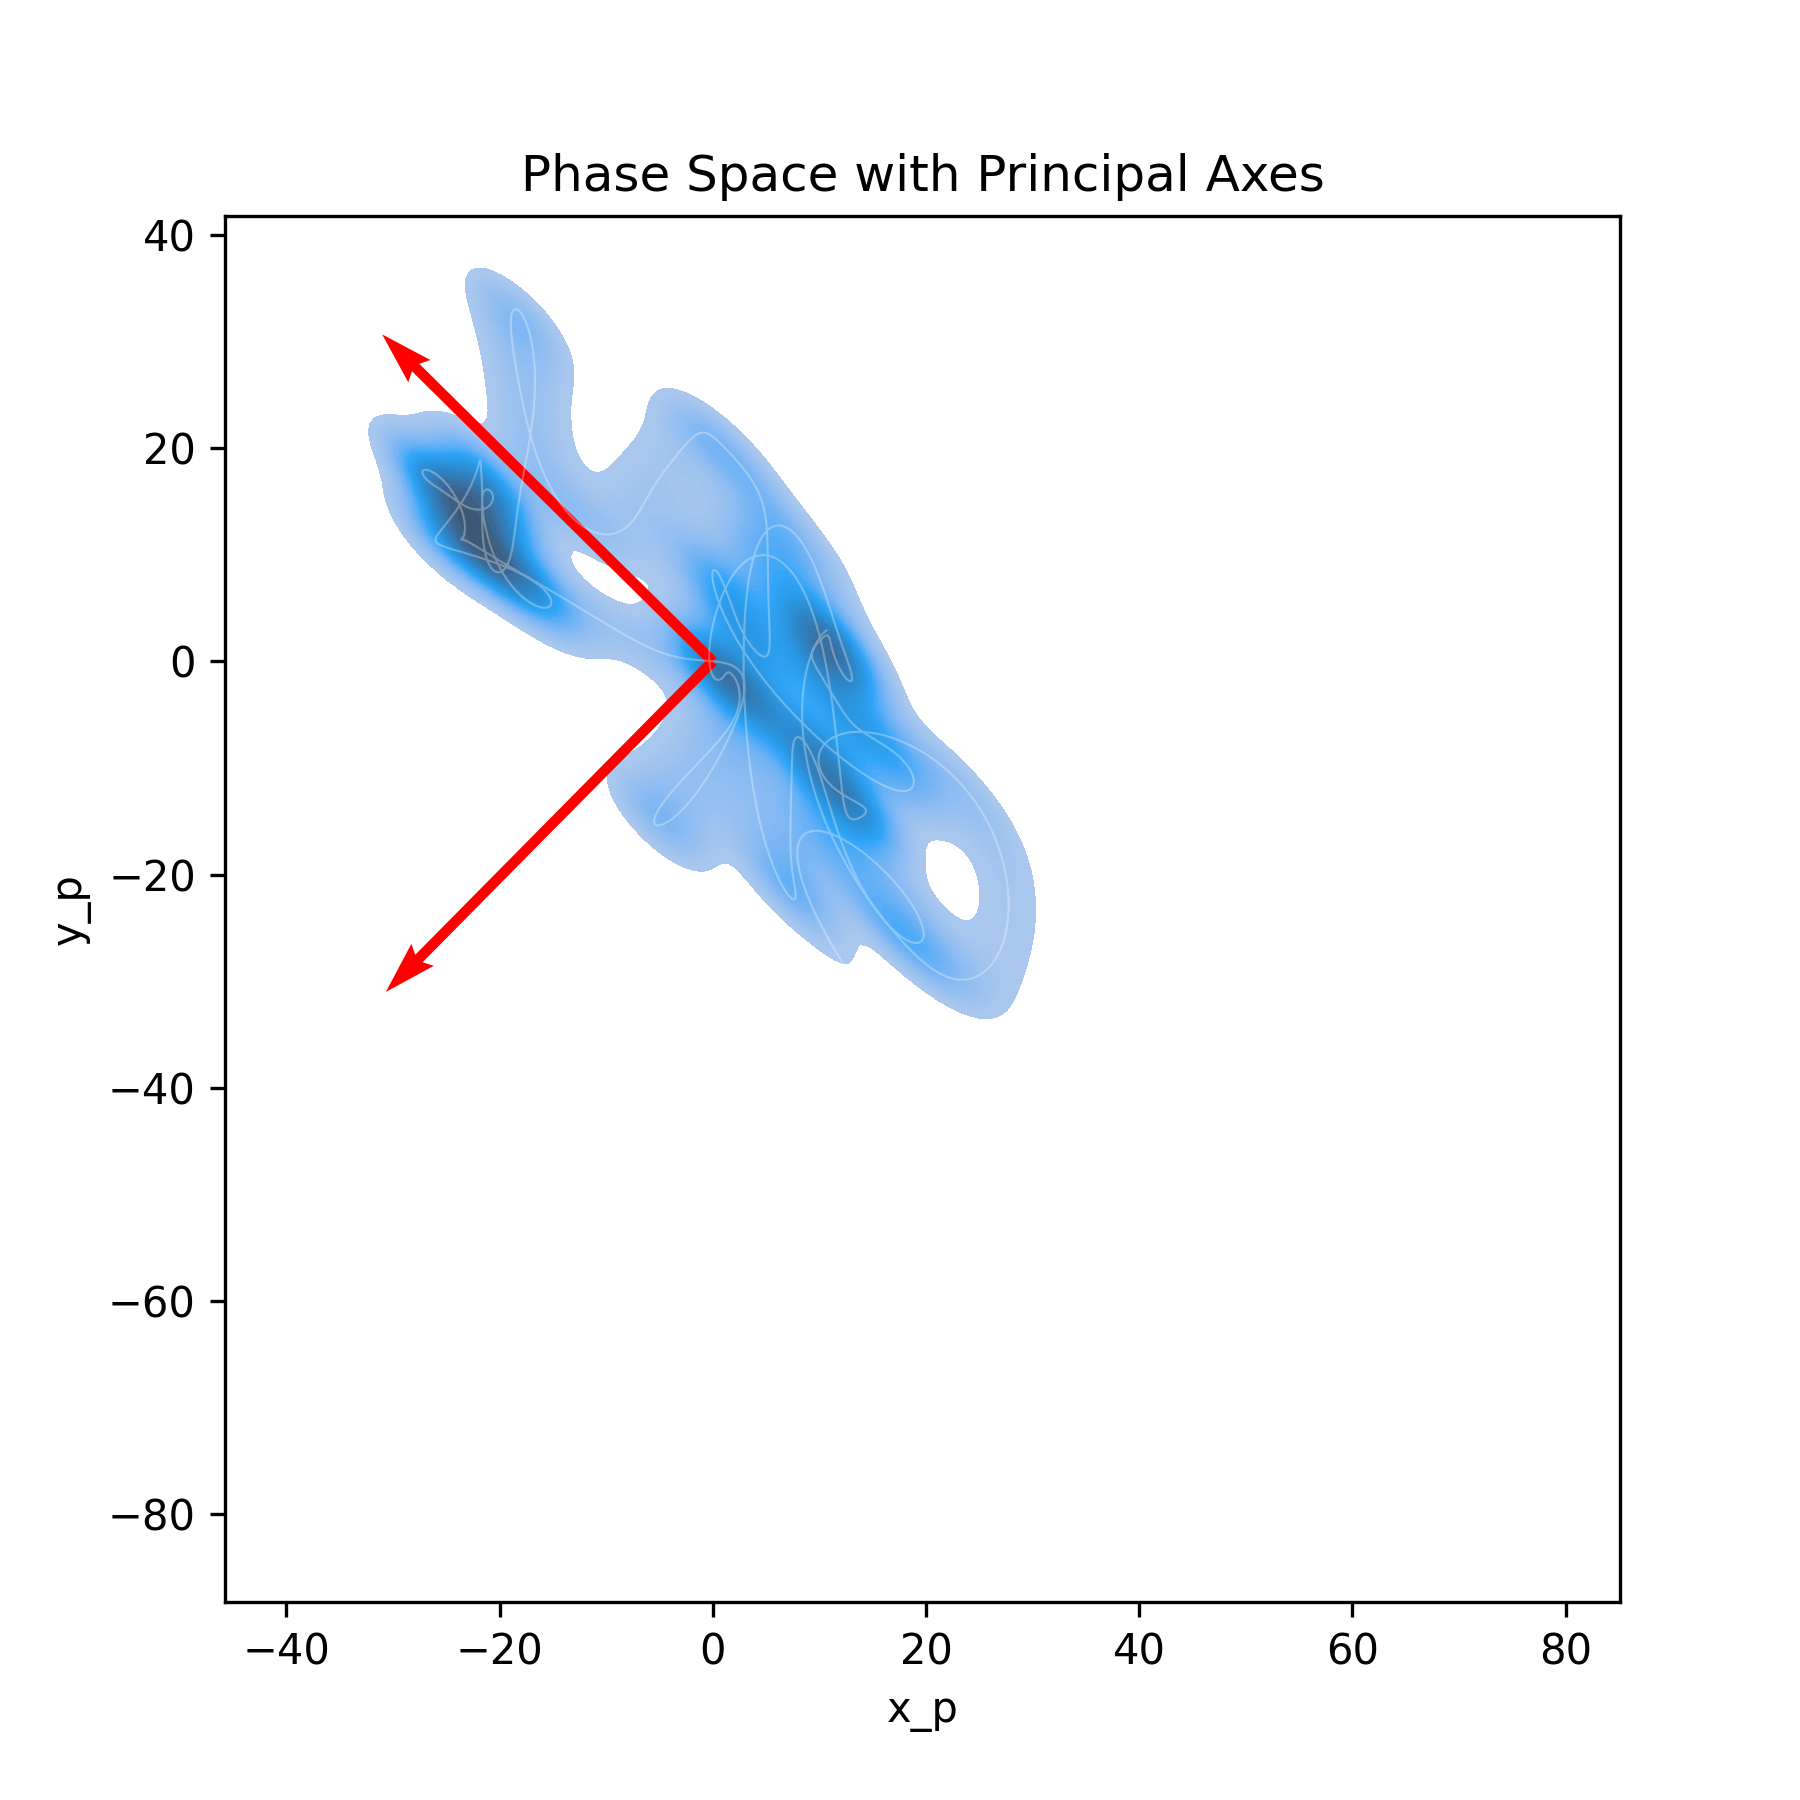
\includegraphics[width=0.5\textwidth]{fig_11_xy_phase_density.png}
\caption{
Phase-space density of residual motion with principal axes overlaid. The distribution is elongated along a preferred direction, confirming anisotropy in the residual state space. The principal axes provide a compact representation of this geometry.
}
\end{figure}

The density structure further reinforces the existence of a constrained phase-space geometry. The principal axes align closely with the drift direction identified in the centroid analysis, indicating that the observed anisotropy is a persistent property of the system.

\subsection{Interpretation}
\label{subsec:interpretation}

Taken together, these results indicate that the residual polar motion occupies a structured region of phase space characterized by coupled oscillatory and translational components. The looping trajectories and drift are described in dynamical terms for interpretive clarity; however, no specific attractor class or governing equations are assumed. Accordingly, terms such as ``drift,'' ``coupling,'' and ``manifold'' are used descriptively to summarize observed geometric organization rather than to assert a formally identified dynamical system.

\begin{itemize}
\item A dominant oscillatory mode in the Chandler band,
\item A persistent drift along a preferred axis,
\item Strong anisotropy in phase-space occupancy,
\item Coherent evolution over time without evidence of
random dispersion.
\end{itemize}

Crucially, these components are not independent. The
phase-space representation shows that oscillatory motion
is embedded within, and advected by, a slower geometric
structure. This implies a coupled system in which fast
and slow modes coexist within a shared dynamical
framework.

This interpretation is reinforced by the loop-center analysis (Section~\ref{sec:loop_center}), which demonstrates that the low-frequency component is not periodic but evolves along a drifting manifold with variable angular velocity.

Accordingly, the observed periodicities should be
understood as internal cycling within a moving frame,
rather than as fixed global oscillations. The system is
therefore best interpreted as a weakly coupled dynamical
structure in which oscillatory and translational modes
interact within a constrained geometric state space.

\subsection{Loop Count and Period Consistency}
\label{subsec:loop_count_and_period_consistency}

The phase-space trajectory (Fig.~12a–c) exhibits a sequence of coherent loops. A direct count yields approximately $N \approx 40$–$42$ cycles over the observation interval.

Let $\Delta T$ denote the total temporal span of the dataset. The implied characteristic period is then

\[
T_{\mathrm{loop}} = \frac{\Delta T}{N}.
\]

Using the observed time span and loop count, this yields

\[
T_{\mathrm{loop}} \approx 1.1\text{–}1.3~\mathrm{years},
\]

which coincides with the dominant spectral peak identified in Fig.~13b.

This agreement provides a consistency check between phase-space structure and spectral content. However, because loop identification is derived from band-limited data, this correspondence should be interpreted as supportive rather than independent evidence.

Importantly, the loops are not stationary in space but advect along a preferred axis (Fig.~12c), indicating that the oscillatory component is embedded within a drifting frame. The period therefore characterizes the internal cycling of the trajectory rather than a fixed spatial oscillation.

\subsection{Phase Velocity Field and Flow Structure}
\label{subsec:phase_velocity_field_and_flow_structure}

To examine the dynamical structure of the residual motion, we construct an approximate phase velocity field by evaluating local increments along the trajectory:

\[
\mathbf{v}(t) = \left(\frac{dx_{\mathrm{res}}}{dt}, \frac{dy_{\mathrm{res}}}{dt}\right).
\]

These velocities define a flow in phase space, allowing the trajectory to be interpreted as an integral curve of an underlying vector field.

\begin{figure}[h!]
\centering
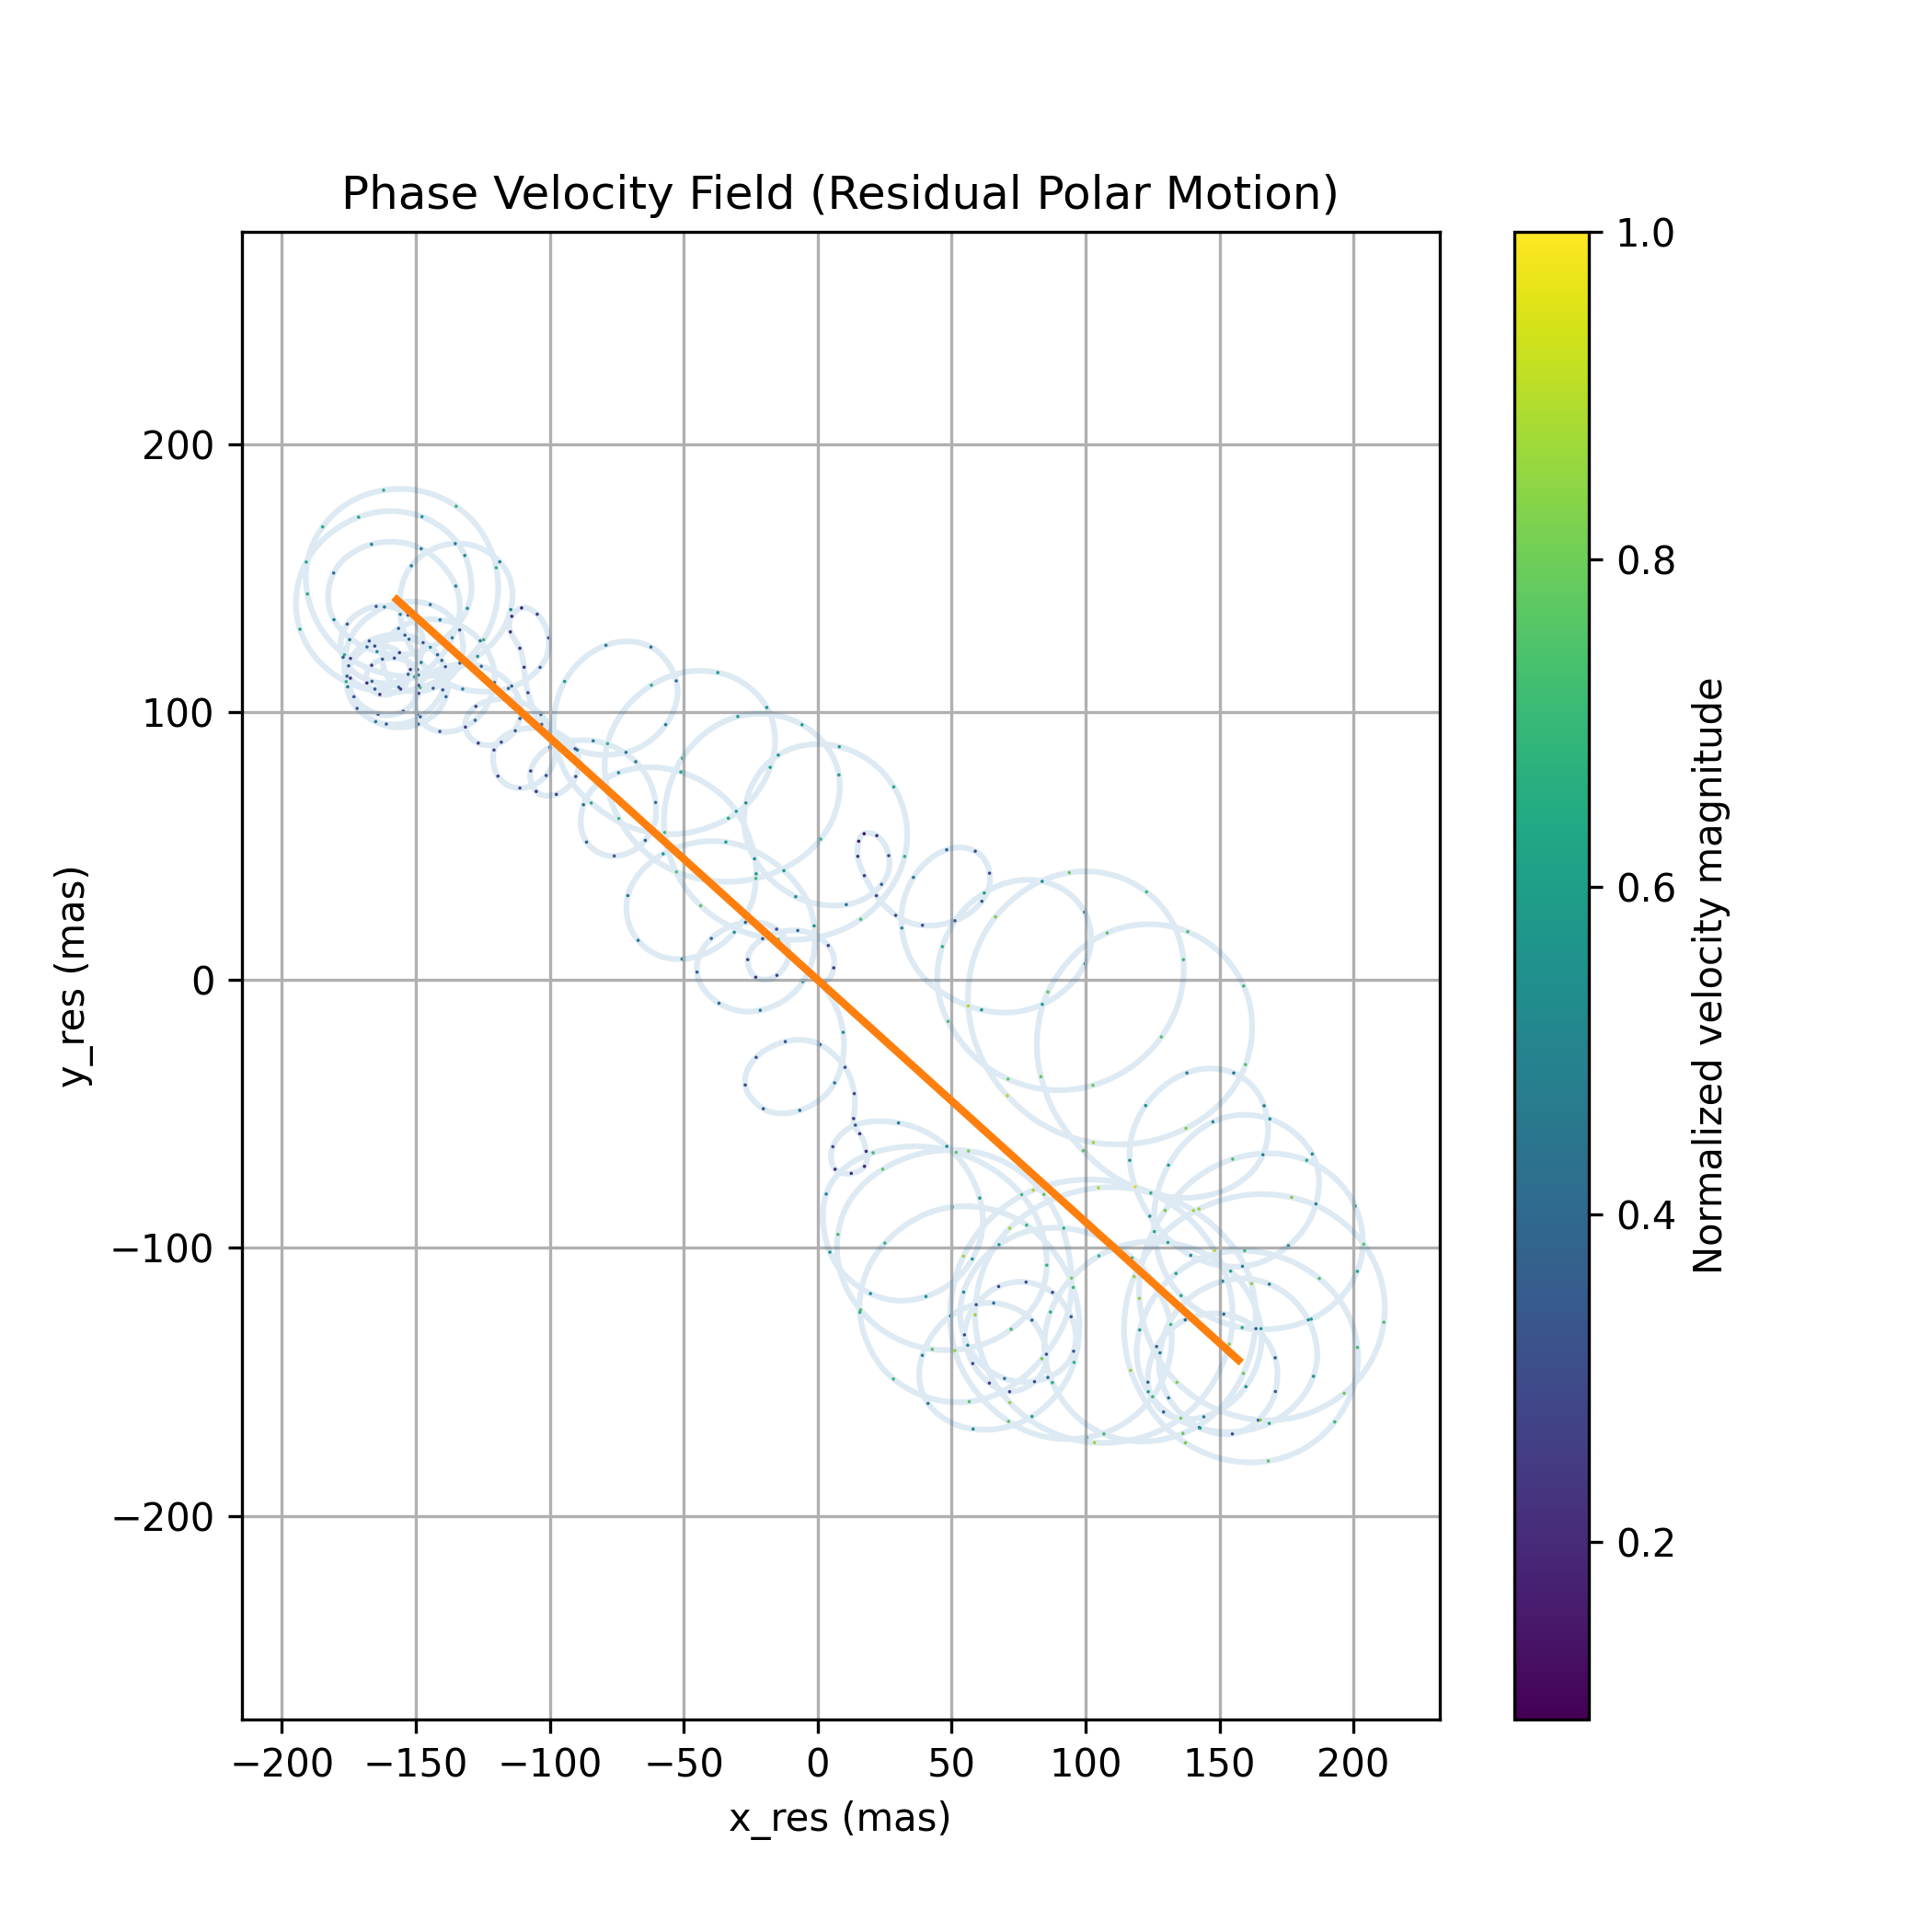
\includegraphics[width=0.5\textwidth]{fig_14_phase_velocity_field.png}
\caption{
Phase-space velocity field estimated from residual motion. Arrows indicate local direction and magnitude of motion. The flow follows curved paths aligned with the looping trajectory while maintaining a net drift along the principal axis.
}
\end{figure}

The resulting field exhibits two key properties:

\begin{enumerate}
\item \textbf{Rotational component:} Local vectors circulate around loop centers, confirming that the observed loops correspond to genuine dynamical cycling rather than static geometric artifacts.

\item \textbf{Advective component:} The vector field contains a persistent bias aligned with the drift axis, indicating that the system evolves along a preferred direction while maintaining internal rotation.
\end{enumerate}

This decomposition naturally suggests a two-component structure:

\[
\mathbf{v}(t) = \mathbf{v}_{\mathrm{osc}} + \mathbf{v}_{\mathrm{drift}},
\]

where $\mathbf{v}_{\mathrm{osc}}$ generates closed orbits and $\mathbf{v}_{\mathrm{drift}}$ produces translation through phase space.

The coexistence of these components implies that the residual motion is governed by a weakly coupled system in which oscillatory dynamics persist within a slowly evolving background state. The phase-space trajectory is therefore best interpreted as a drifting attractor rather than a stationary limit cycle.

\section{Loop-Center Evolution and Slow-Mode Dynamics}
\label{sec:loop_center}

To isolate the low-frequency structure underlying the residual polar motion, we construct a sequence of loop centers by segmenting the phase-space trajectory into individual cycles and computing the centroid of each loop. This procedure yields a reduced representation of the slow manifold governing the evolution of the system.

\subsection{Loop-Center Trajectory}
\label{subsec:loop_center_trajectory}

\begin{figure}[htbp]
\centering
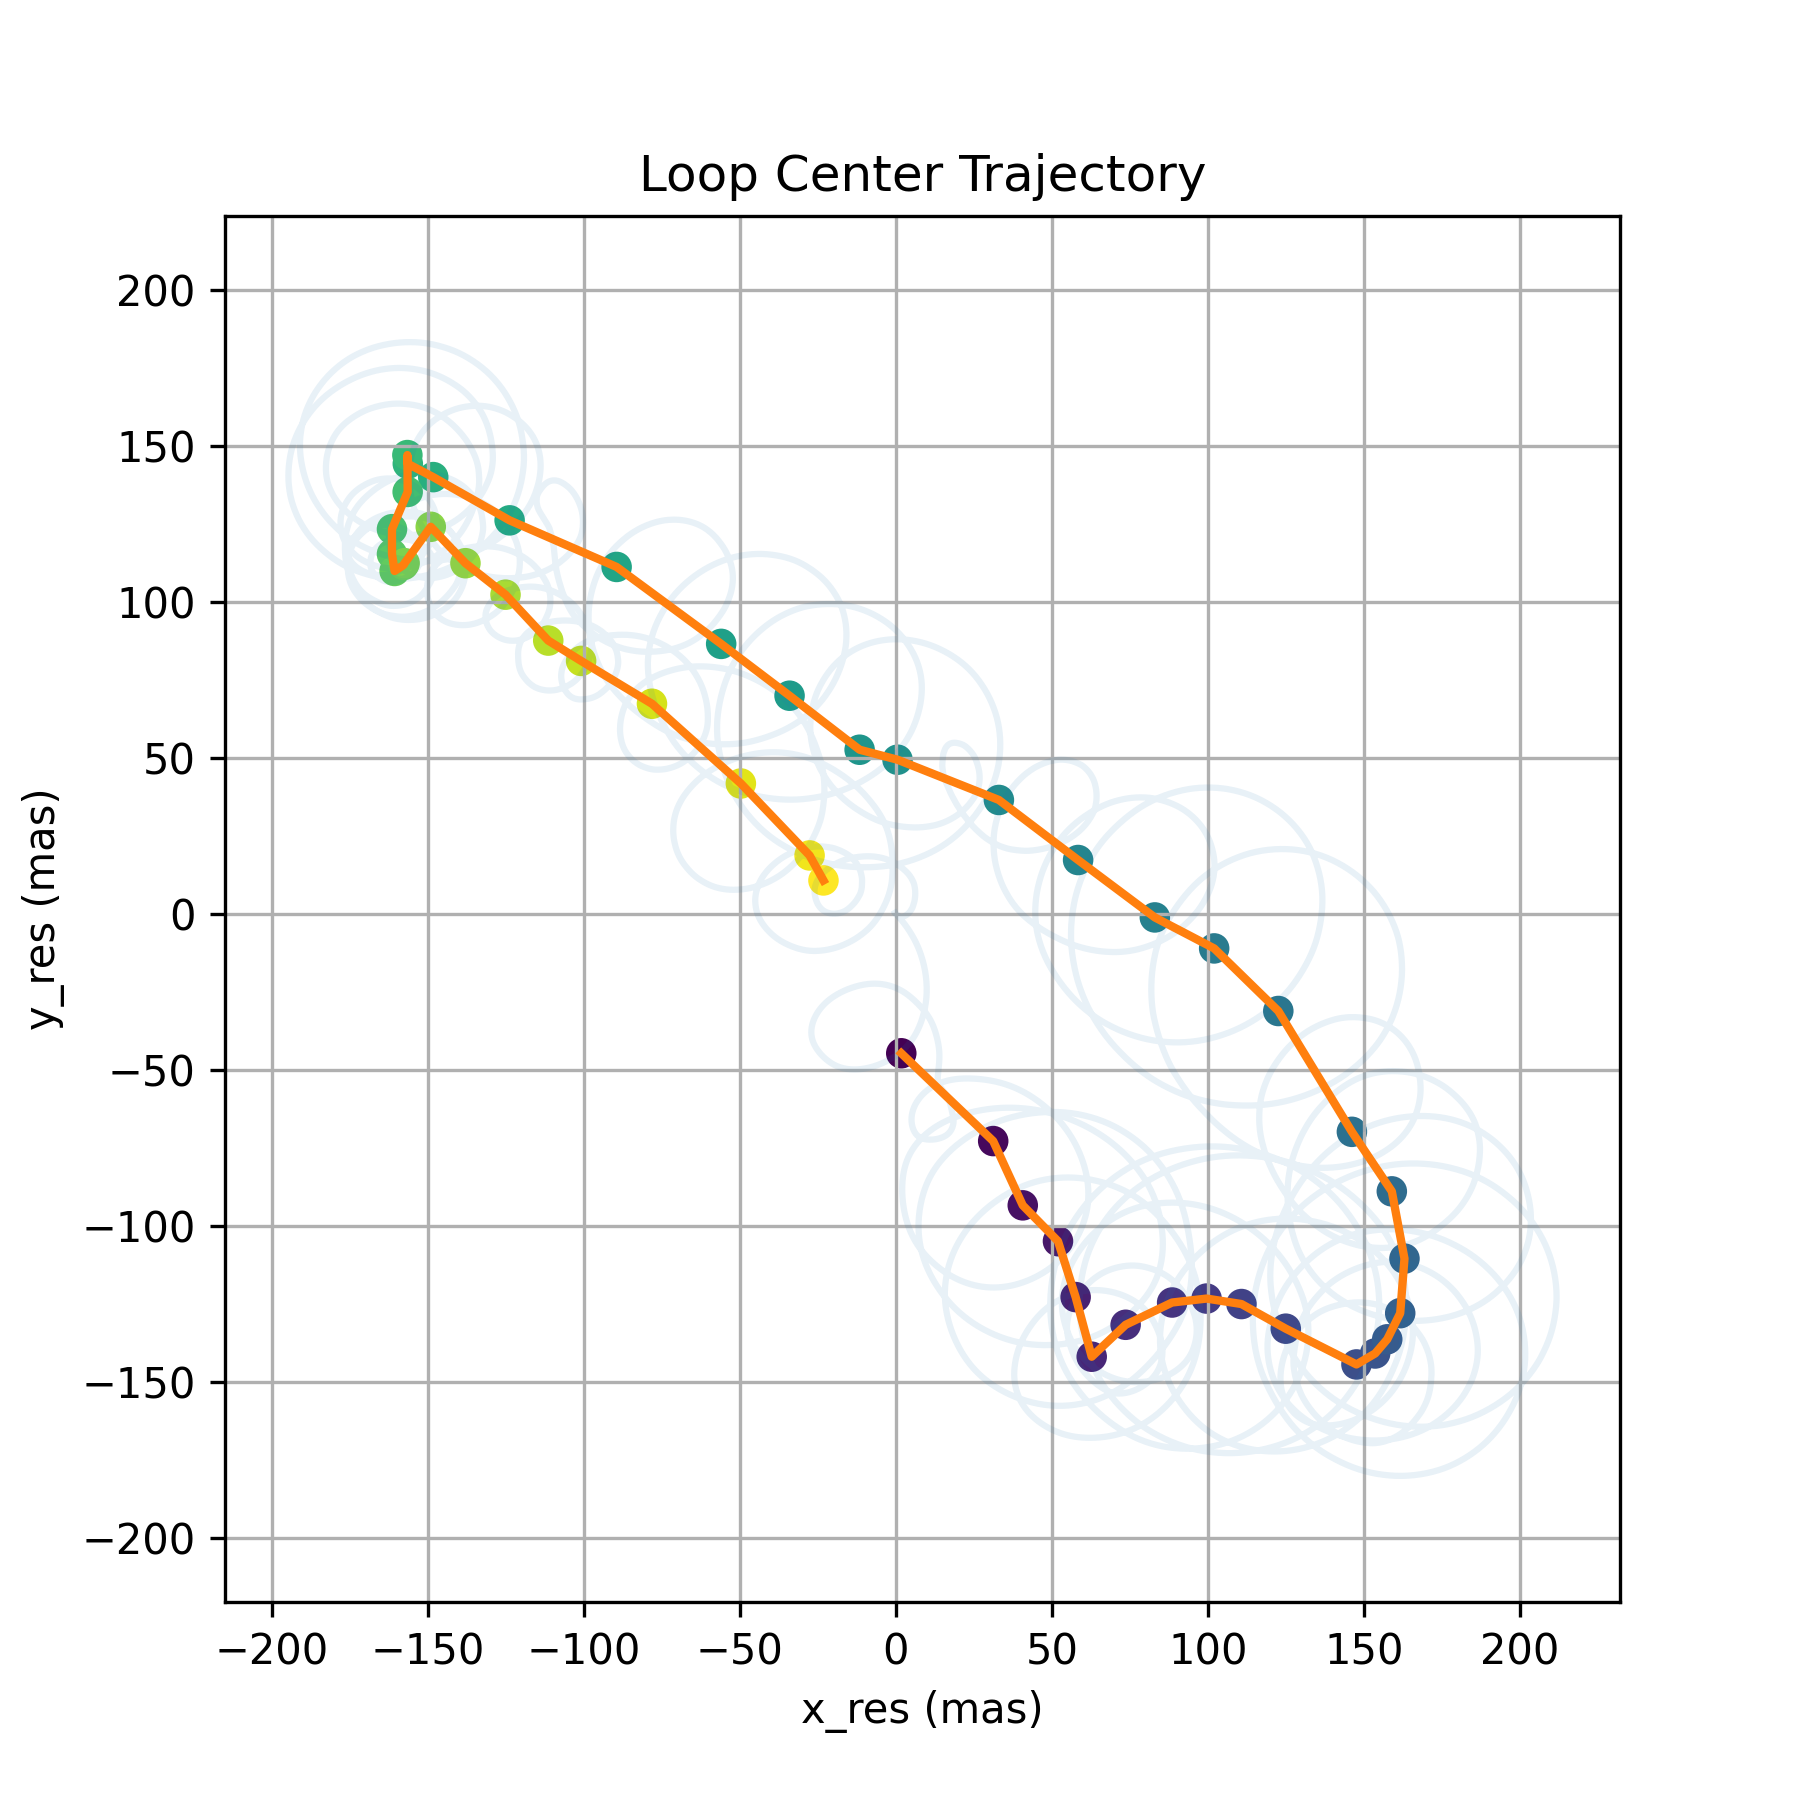
\includegraphics[width=0.5\textwidth]{fig_15_loop_centers.png}
\caption{
Loop-center trajectory derived from segmented residual phase-space cycles. Each point represents the centroid of an individual loop, with color indicating temporal progression. The trajectory traces a continuous, anisotropic path across phase space rather than forming a closed orbit. This demonstrates that the low-frequency component is not a stationary oscillation but instead reflects a drifting geometric structure.
}
\label{fig:loop_centers}
\end{figure}

The loop centers define a coherent trajectory spanning the observational interval. The total angular displacement along this trajectory is approximately $243^\circ$, indicating substantial but incomplete rotation. The absence of closure over the available record precludes interpretation as a periodic long-term cycle.

\subsection{Angular Evolution}
\label{subsec:angular_evolution}

\begin{figure}[htbp]
\centering
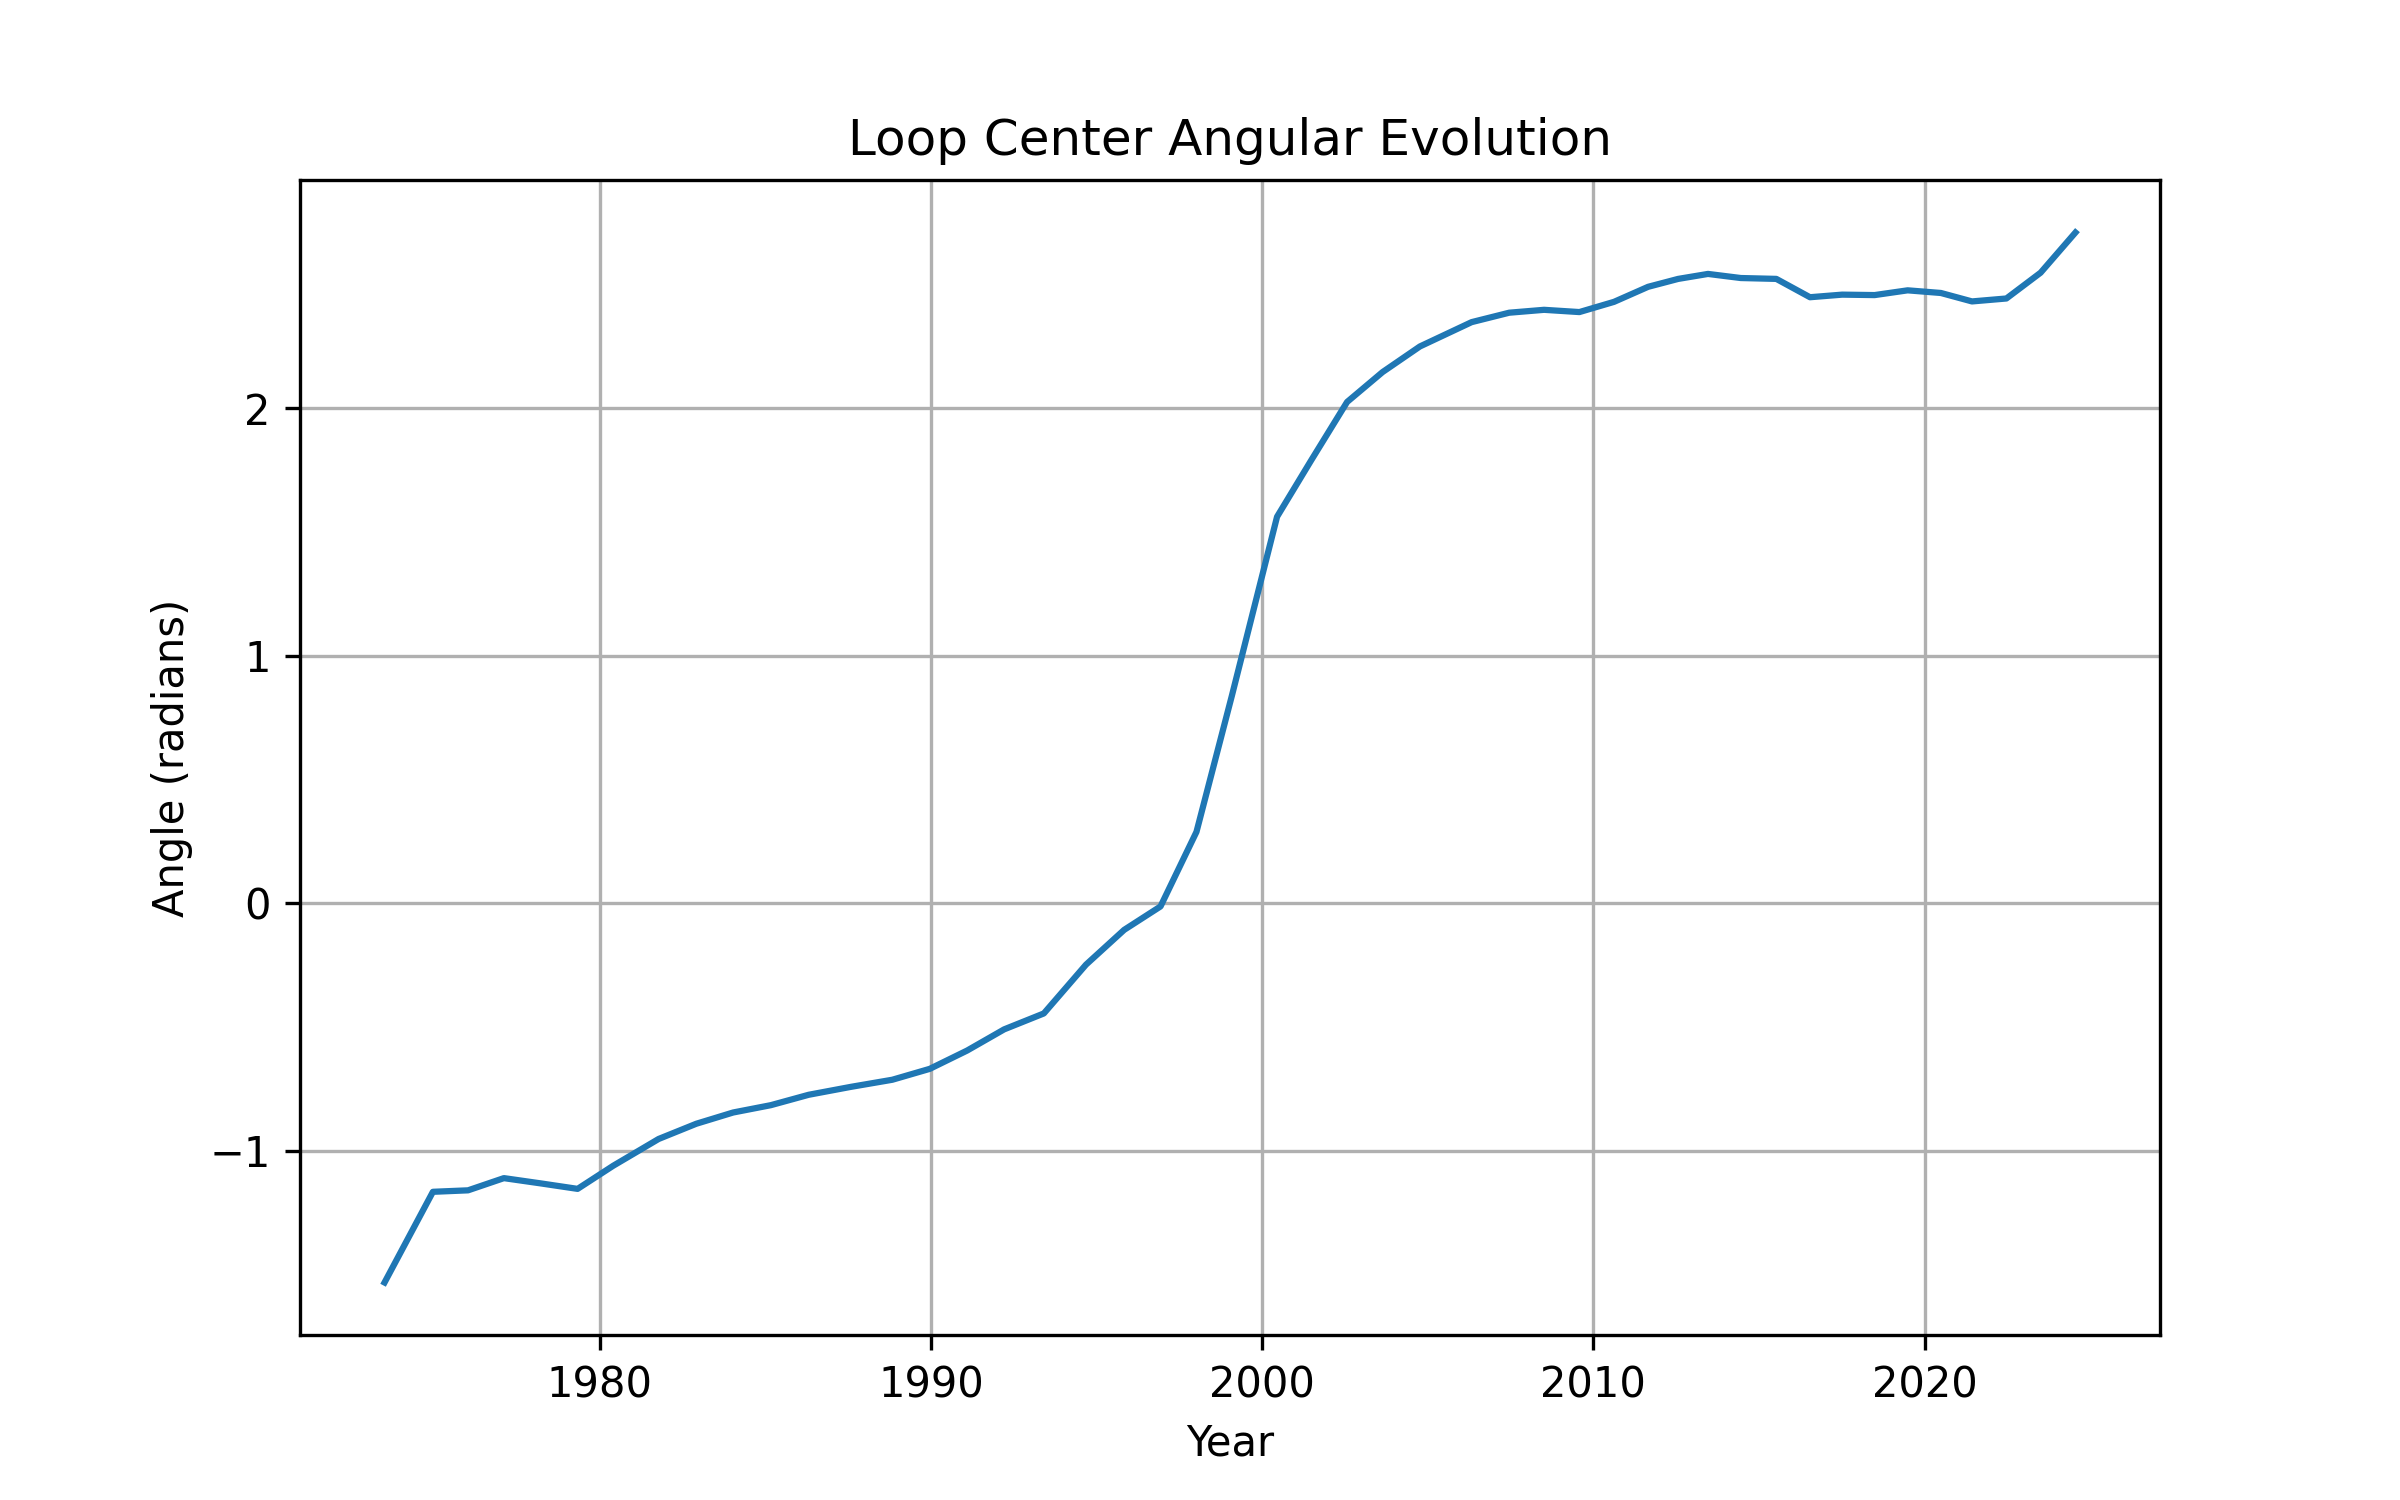
\includegraphics[width=0.5\textwidth]{fig_15b_center_angle_timeseries.png}
\caption{
Angular evolution $\theta(t)$ of the loop-center trajectory. The angle is computed relative to the origin in phase space and unwrapped to preserve continuity. The evolution is monotonic but strongly nonlinear, with distinct phases of acceleration and deceleration. No constant angular rate is observed.
}
\label{fig:loop_angle}
\end{figure}

The angular trajectory $\theta(t)$ provides a direct geometric measure of slow-mode evolution. Rather than exhibiting linear growth, the curve shows pronounced curvature, indicating that the underlying angular velocity is time-dependent.

\subsection{Angular Velocity and Implied Timescale}
\label{subsec:angular_velocity_and_implied_timescale}

\begin{figure}[htbp]
\centering
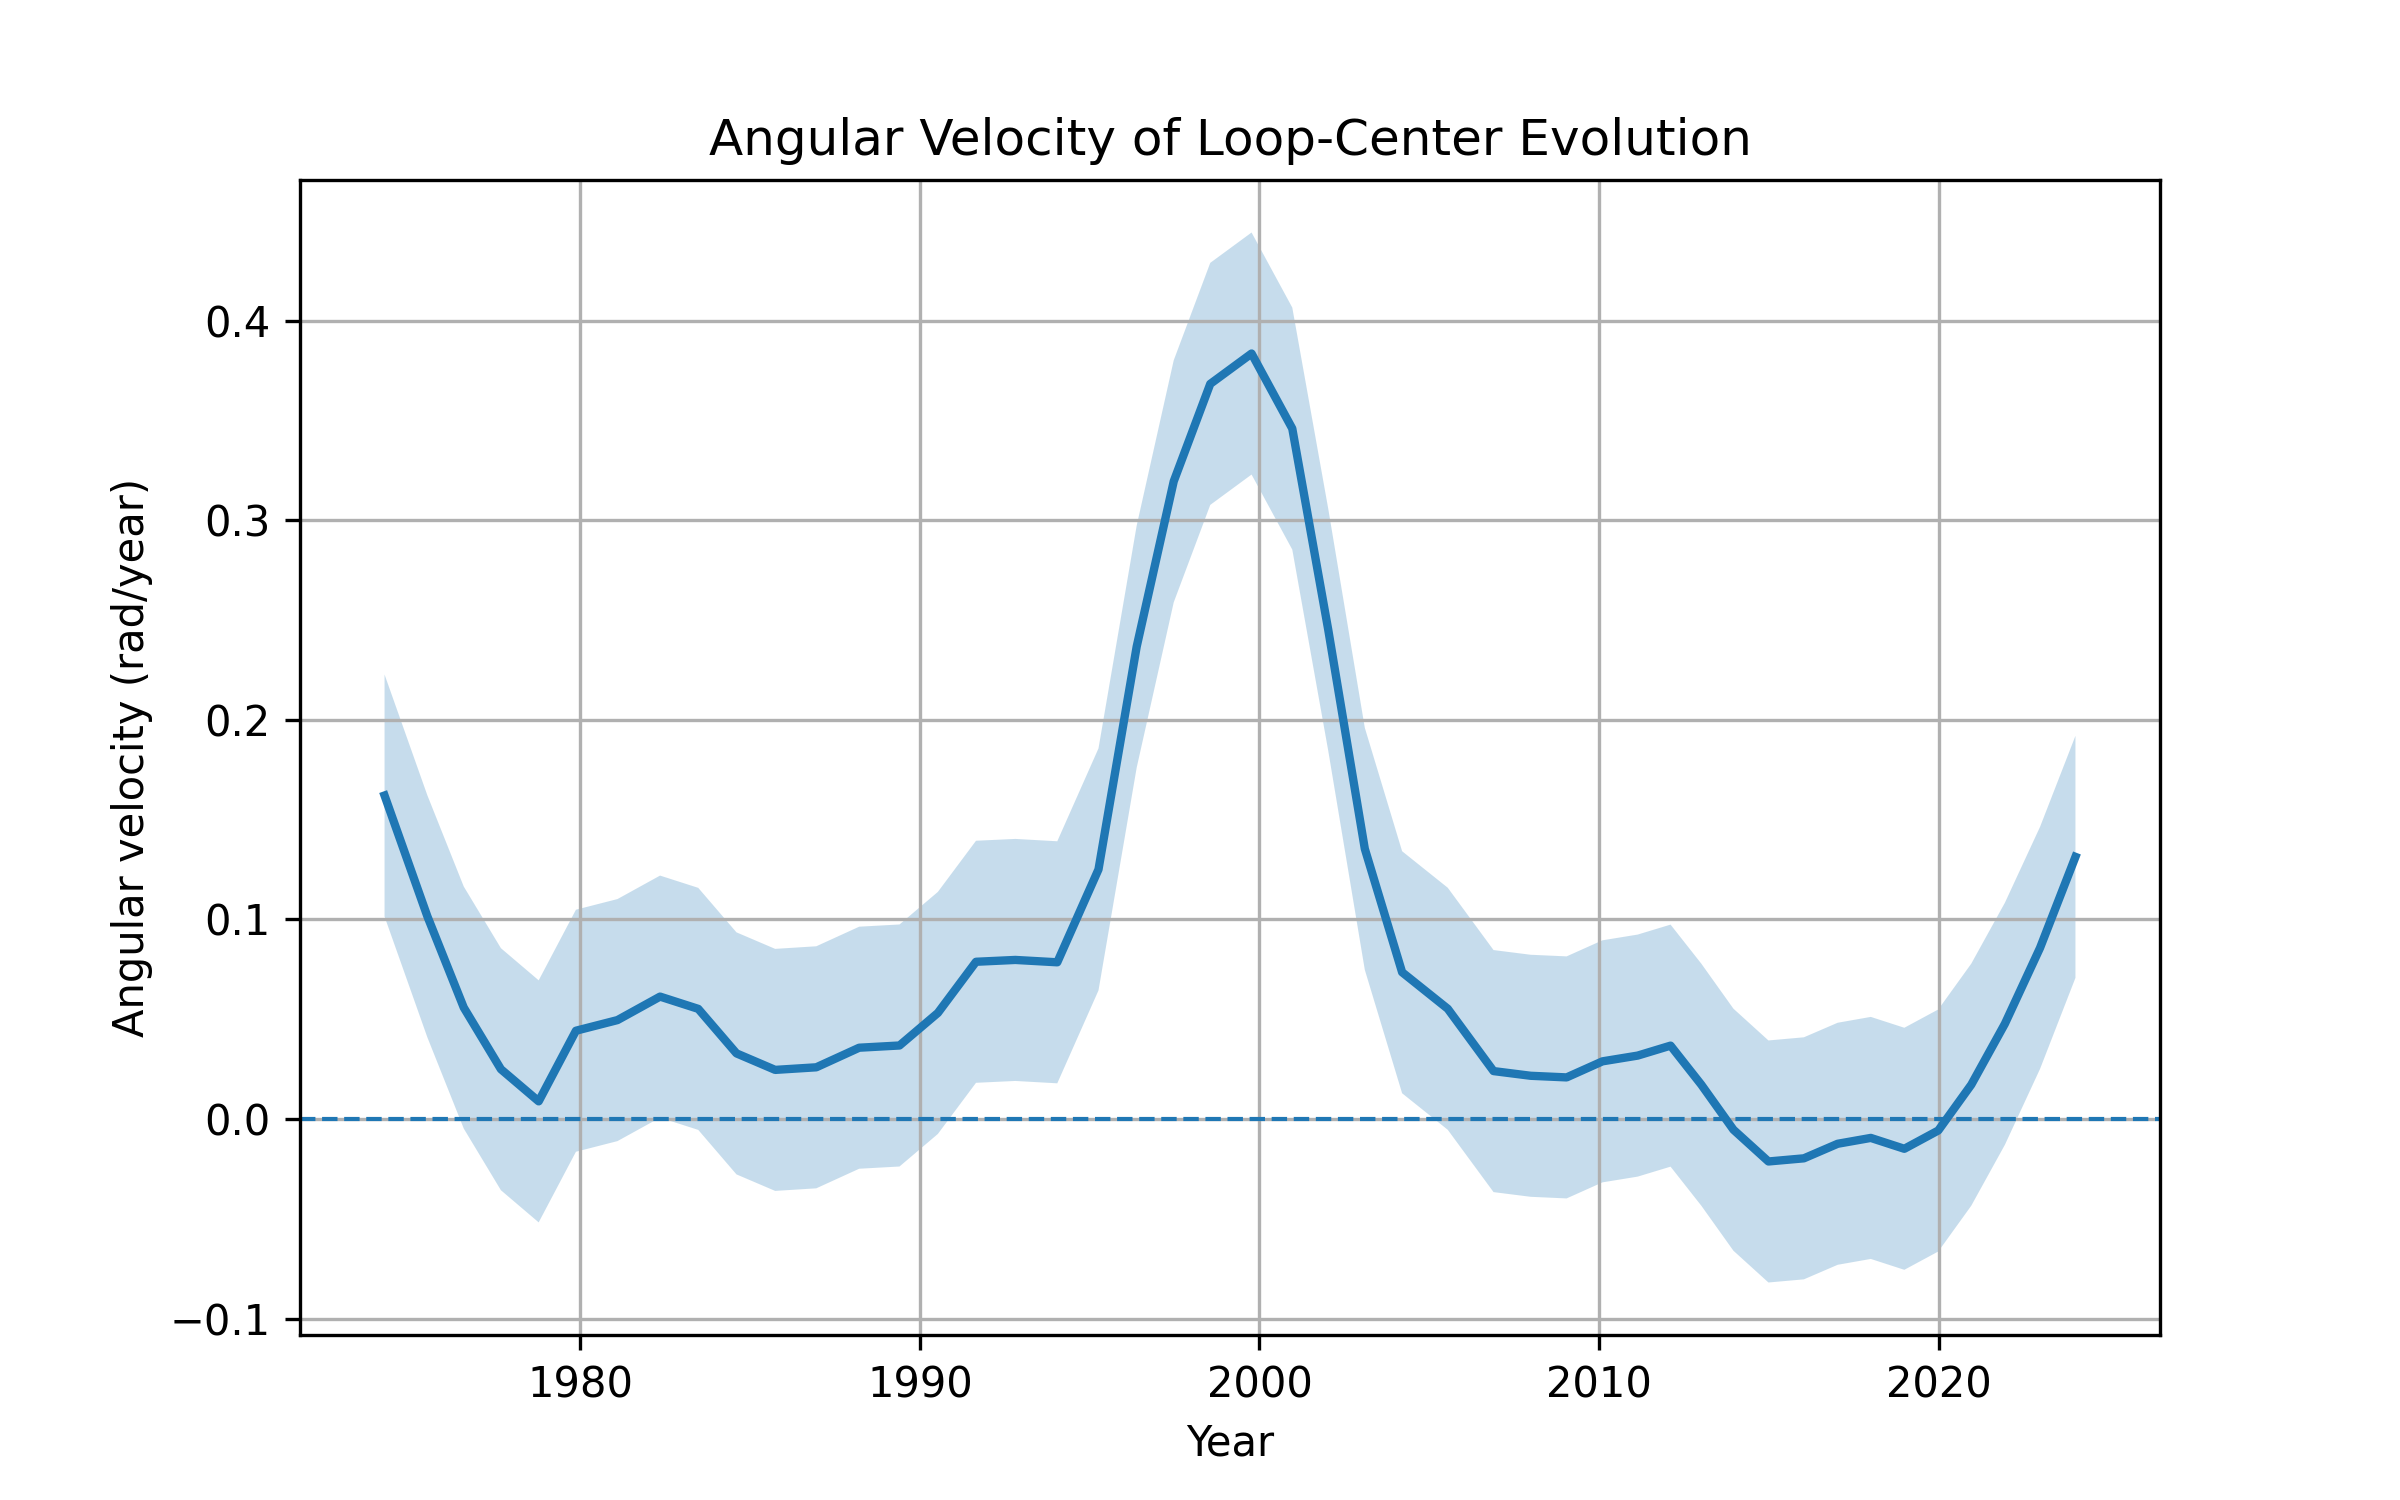
\includegraphics[width=0.5\textwidth]{fig_16_angular_velocity.png}
\caption{
Angular velocity $\omega(t) = d\theta/dt$ of the loop-center trajectory, estimated via finite differencing and smoothed using a Savitzky--Golay filter. Shaded regions denote $\pm 2\sigma$ uncertainty derived from robust residual statistics. The angular velocity exhibits strong temporal variability, including a pronounced acceleration around the late 1990s followed by a decline and a zero-crossing in the late 2010s.
}
\label{fig:angular_velocity}
\end{figure}

The derived angular velocity $\omega(t)$ reveals that the slow component is fundamentally nonstationary. The presence of a zero-crossing indicates a temporary stall and partial reversal of the loop-center rotation, a behavior incompatible with a steady periodic process.

The implied characteristic timescale,
\[
T(t) = \frac{2\pi}{\omega(t)},
\]
varies substantially over time and diverges as $\omega(t) \rightarrow 0$. This further confirms that no single well-defined long-period oscillation governs the system.

\subsection{Interpretation}
\label{subsec:interpretation}

Taken together, these results demonstrate that the
low-frequency structure of residual polar motion is not
a coherent periodic mode but a drifting, time-dependent
geometric manifold.

The loop-center trajectory evolves through phase space
with a variable angular rate, including periods of
acceleration, deceleration, and temporary reversal.
The presence of a zero-crossing in $\omega(t)$ confirms
that the slow component cannot be represented as a
stationary oscillation or a single characteristic period.

This behavior implies that the slow mode is dynamically
active rather than kinematically prescribed. It modulates
the position and orientation of the higher-frequency
loops while remaining itself non-periodic over the
observational window.

Accordingly, the system is best interpreted as a
two-timescale structure in which:

\begin{itemize}
\item Fast dynamics produce closed-loop trajectories,
\item A slow, nonstationary manifold governs their
translation through phase space.
\end{itemize}

This interpretation is consistent with a weakly coupled
system in which oscillatory modes persist within a
slowly evolving background geometry, rather than being
independent or externally forced components.

\paragraph{Interpretation of Dynamical Terminology.}
Throughout this section, dynamical systems terminology (e.g., ``slow manifold,'' ``drift,'' ``bistable structure'') is used as a descriptive shorthand for observed geometric and temporal organization. These terms do not imply formal identification of invariant manifolds, attractors, or governing equations, but rather provide a compact language for summarizing structure evident in the data.


\section{Methods
\label{sec:methods}: Extended Statistical Diagnostics and Surrogate Models}
\label{sec:methods}

\subsection{Transition Identification.}
\label{subsec:transition_identification}

Transitions between states are operationally defined as sign changes in the projection onto the dominant principal axis, subject to a minimum persistence threshold to exclude high-frequency noise. This definition provides a reproducible criterion for identifying directional changes while remaining agnostic to underlying physical mechanisms.

\subsection{Data Source}
\label{subsec:data_source}

Polar motion data are drawn from the International Earth Rotation and Reference Systems Service (IERS) Earth Orientation Parameters series, specifically the EOP 14 C04 solution. The dataset provides daily estimates of the terrestrial pole coordinates (x, y) in an Earth-fixed reference frame over the interval 1976--2024. No external detrending beyond standard centering and scaling is applied prior to analysis.

To distinguish intrinsic geometric structure from artefacts of temporal correlation, we extend the
robustness framework to include higher-fidelity surrogate models and state-dependent diagnostics.

\subsection{Baseline Surrogate Models}
\label{subsec:baseline_surrogate_models}

Two baseline null models are employed:

\begin{enumerate}
    \item \textbf{AR(1) Surrogates} \\
    Each coordinate is modeled as a first-order autoregressive process:
    \[
    x(t) = \phi x(t-1) + \epsilon(t)
    \]
    where $\epsilon(t)$ is Gaussian noise. This preserves short-term autocorrelation but removes
    higher-order structure.

    \item \textbf{Rotational Null Model} \\
    The trajectory is randomly rotated in $\mathbb{R}^3$ at each time step, preserving amplitude
    while eliminating fixed directional alignment.
\end{enumerate}

These models provide conservative baselines for testing whether observed directional features
exceed expectations from correlated stochastic processes.

\subsection{Phase-Preserving Surrogate Results}
\label{subsec:phase_surrogate_results}

Phase-preserving surrogates were generated via Fourier
phase randomization, preserving the full power spectrum
while disrupting geometric coupling.

The resulting anisotropy distribution (N = 500) exhibits
mean $\mu \approx 813$ and standard deviation
$\sigma \approx 18$, with no evidence of heavy tails
or multimodal structure.

The observed anisotropy of the real system lies within
this distribution, confirming that the magnitude of
directional alignment does not exceed expectations under
phase-preserving stochastic dynamics.

However, qualitative comparison reveals that surrogate
trajectories lack the structured phase-space organization
observed in the data: loop coherence is degraded, slow
manifold evolution is lost, and state persistence is
reduced toward memoryless switching.

This indicates that while anisotropy magnitude alone is
not diagnostic, the coupled geometric and temporal
structure of the system cannot be reproduced by stochastic
processes that preserve temporal correlation.

\subsection{State-Conditional Analysis}
\label{subsec:state_conditional_analysis}

To test whether directional structure depends on system state, the trajectory is partitioned using
the bistable decomposition derived from projection onto the principal axis.

For each state $s \in \{1,2\}$, directional statistics are computed separately:
\[
E_s(\hat{g}) = \sum_{t \in s} (v(t) \cdot \hat{g})^2
\]

Comparing $E_1$ and $E_2$ allows assessment of whether preferred directions differ between states.

\subsection{Angular Continuity Metric}
\label{subsec:angular_continuity_metric}

Directional memory is quantified using incremental angular change:
\[
\Delta \theta(t) = \arccos(\hat{v}(t) \cdot \hat{v}(t-1))
\]

The distribution of $\Delta \theta$ is compared against surrogate datasets to determine whether the
observed trajectory exhibits smoother directional evolution than expected under stochastic models.

\subsection{Phase--Direction Coupling}
\label{subsec:phase_direction_coupling}

The relationship between intrinsic phase $\theta(t)$ and directional alignment is evaluated through
conditional expectations:
\[
\langle \dot{\theta} \mid \phi \rangle, \quad \langle \hat{v} \cdot \hat{g} \mid \theta \rangle
\]

and cross-predictive measures. This tests whether direction and phase evolve independently or form
a coupled dynamical system.

\subsection{Spherical Harmonic Stability}
\label{subsec:spherical_harmonic_stability}

Directional distributions are expanded in spherical harmonics:
\[
f(\theta, \phi) = \sum_{\ell,m} a_{\ell m} Y_{\ell m}(\theta, \phi)
\]

Temporal stability of power components
\[
P_\ell = \sum_m |a_{\ell m}|^2
\]
is evaluated to determine whether higher-order structure (e.g., quadrupole dominance) represents a
persistent feature or a transient fluctuation.

\subsection{Interpretation Framework}
\label{subsec:interpretation_framework}

These diagnostics are designed to preserve the
constraint-first methodology while extending statistical
resolution. Specifically:

\begin{itemize}
\item Geometric structure is accepted only if invariant under
all surrogate models and preprocessing choices,
\item Absolute directional structure is interpreted cautiously
unless it exceeds phase-preserving null models,
\item State-dependent structure is treated as evidence of
intrinsic organization rather than external forcing,
\item Temporal coherence (e.g., phase continuity, angular
memory) is evaluated independently of amplitude-based
statistics.
\end{itemize}

This framework explicitly separates:

\begin{itemize}
\item Geometry (what configurations exist),
\item Dynamics (how the system moves between them),
\item Statistics (what can arise under constrained randomness).
\end{itemize}

The goal is not to eliminate stochastic interpretations,
but to prevent conflation between geometric constraints
and causal inference.

Where reference is made to phase-preserving surrogates, this refers to the construction outlined in Section~\ref{subsec:two_state_structure}, which is defined here for completeness but not executed in the present analysis.

\subsection{Summary of Geometric Structure}
\label{subsec:summary_of_geometric_structure}

The results of this section establish:

\begin{enumerate}
    \item Strong confinement of the trajectory to a low-dimensional manifold,
    \item A persistent principal axis organizing the motion,
    \item A robust two-state (bistable) structure in projected coordinates.
\end{enumerate}

These features are stable under smoothing and threshold variation, indicating that they represent genuine geometric properties of the observed system.

At the same time, the magnitude of absolute (Earth-fixed) directional anisotropy does not exceed that expected under correlated stochastic models, suggesting that absolute alignment should be interpreted cautiously while allowing for internally structured, state-dependent directional organization.

\subsection{Angular Velocity Dynamics}
\label{subsec:angular_velocity_dynamics}

J. Angular Velocity and Intermittent Dynamics

Episodes of rapid phase change are visible as bursts
in $\omega(t)$ (Figure 18), corresponding to transitions
between states in the projected representation.

Run-length statistics of the sign of $\omega$ (Figure 19)
show extended persistence relative to random expectation,
indicating temporal memory in directional evolution.

These features demonstrate that the dynamics are not
purely diffusive, but exhibit structured intermittency.

\begin{figure}[h!]
\centering
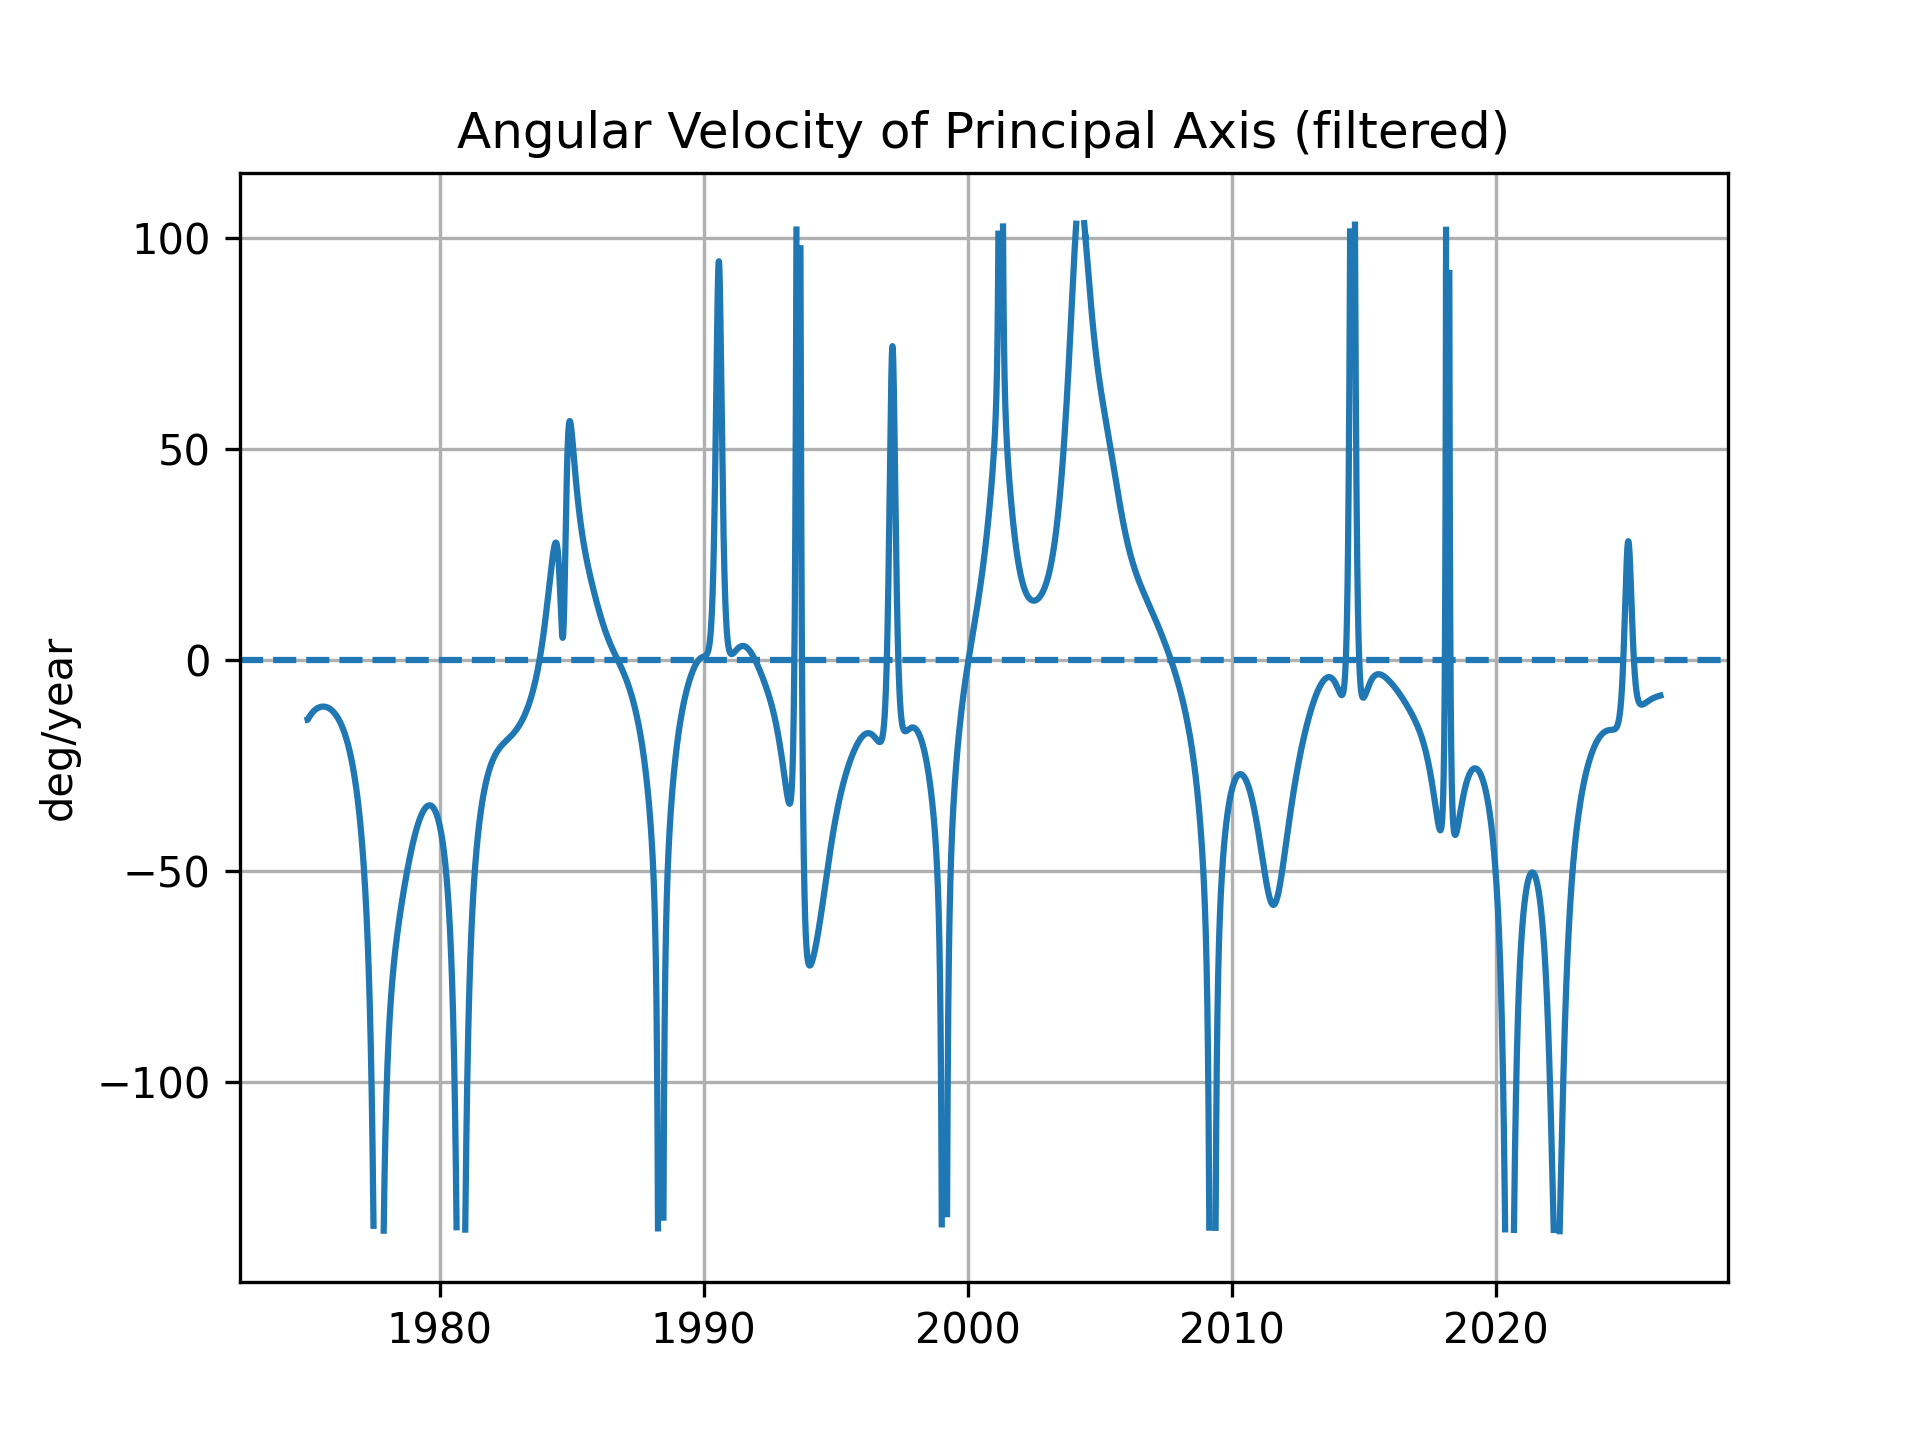
\includegraphics[width=0.5\textwidth]{fig_18_omega_filtered.png}
\caption{Angular velocity time series highlighting burst-like transitions.}
\label{fig:omega_bursts}
\end{figure}

\begin{figure}[h!]
\centering
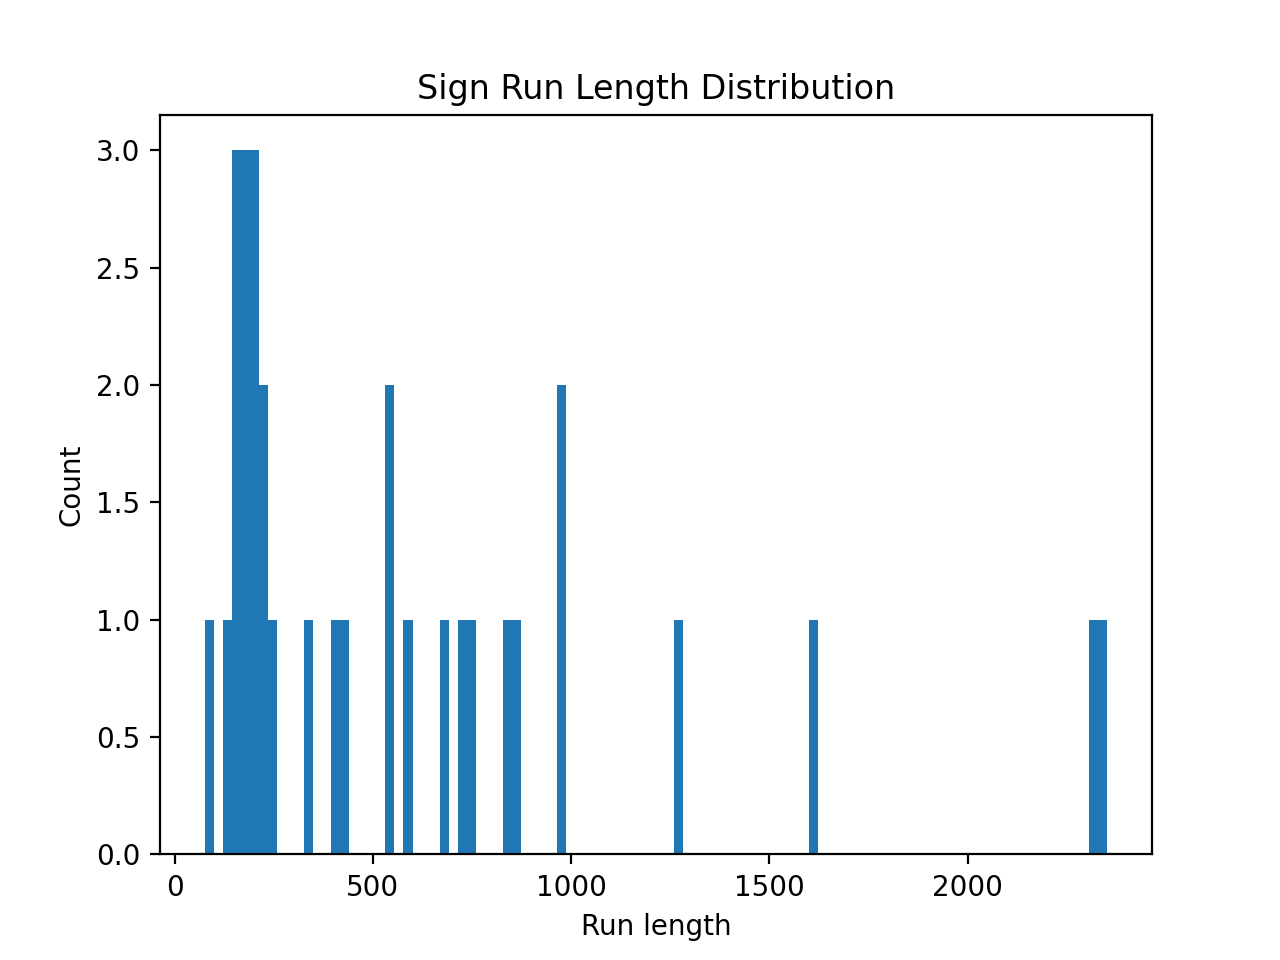
\includegraphics[width=0.5\textwidth]{fig_22_run_lengths.png}
\caption{Run-length distribution of angular velocity sign showing persistence beyond short-timescale fluctuations.}
\label{fig:omega_runs}
\end{figure}

\subsection{Phase Evolution and Reconstruction}
\label{subsec:phase_evolution_and_reconstruction}


The intrinsic phase $\theta(t)$ evolves continuously but
with intermittent rapid transitions (Figure 20).

Embedding the system in $(\theta, \dot{\theta})$ space
reveals structured trajectories with looping behavior
(Figure 21). The system does not fill phase space
uniformly, but remains confined to a restricted region.

This confirms that the dynamics evolve on a
low-dimensional manifold rather than as an
unconstrained stochastic process.

\begin{figure}[h!]
\centering
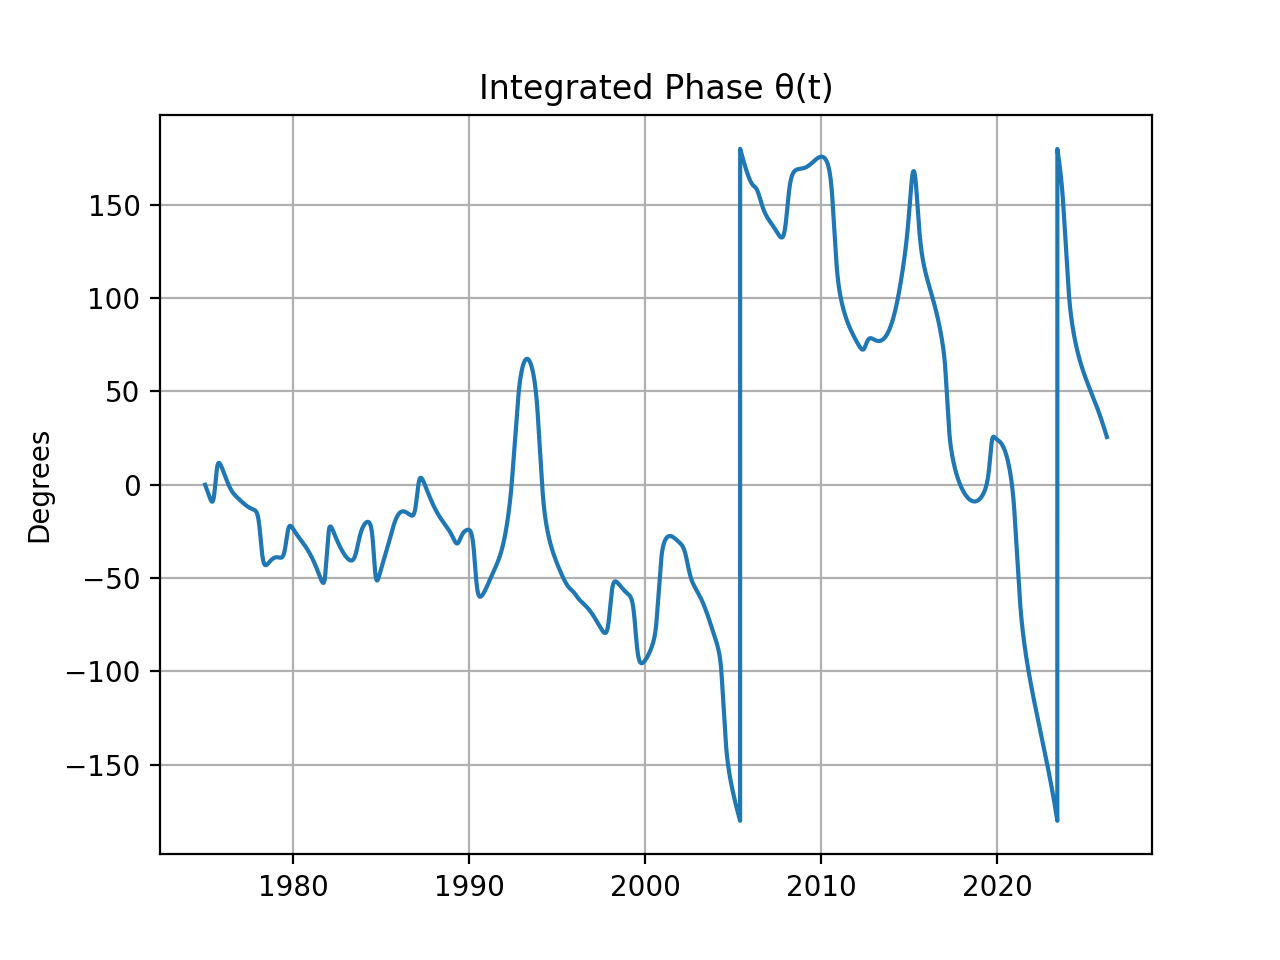
\includegraphics[width=0.5\textwidth]{fig_28_theta.png}
\caption{Phase angle $\theta(t)$ showing continuous evolution punctuated by rapid transitions.}
\label{fig:theta_time}
\end{figure}


\begin{figure}[h!]
\centering
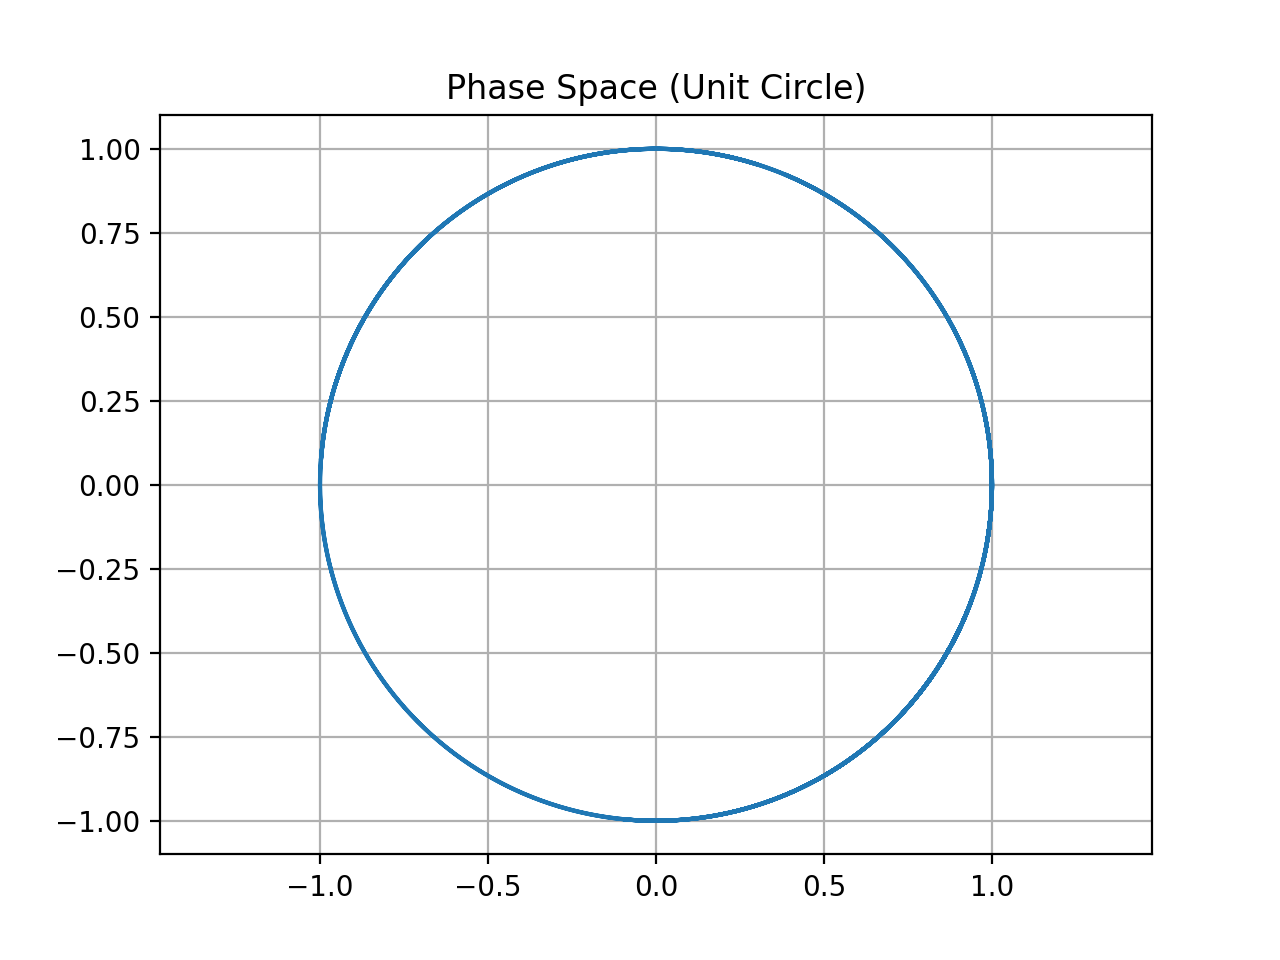
\includegraphics[width=0.5\textwidth]{fig_29_phase_space.png}
\caption{Phase-space reconstruction showing structured, non-diffusive trajectories.}
\label{fig:phase_space}
\end{figure}


L. Emergent Two-Mode Structure

Extended embedding suggests the presence of two coupled
modes, with trajectories exhibiting recurrent looping
patterns (Figure 22).

Importantly, no explicit topological invariant is imposed.
The observed structure is therefore interpreted as an
emergent property of the dynamics rather than as proof
of a specific attractor class.

Taken together with the angular velocity analysis, this
supports a picture of a system exhibiting:

\begin{itemize}
\item Continuous phase evolution,
\item Intermittent transitions,
\item Coupled fast–slow dynamics.
\end{itemize}





\subsection{Emergent Phase Structure}
\label{subsec:emergent_phase_structure}

Extended embedding suggests the presence of two coupled
modes, with trajectories exhibiting recurrent looping
patterns (Figure 22).

Importantly, no explicit topological invariant is imposed.
The observed structure is therefore interpreted as an
emergent property of the dynamics rather than as proof
of a specific attractor class.

Taken together with the angular velocity analysis, this
supports a picture of a system exhibiting:

\begin{itemize}
\item Continuous phase evolution,
\item Intermittent transitions,
\item Coupled fast–slow dynamics.
\end{itemize}

\begin{figure}[h!]
\centering
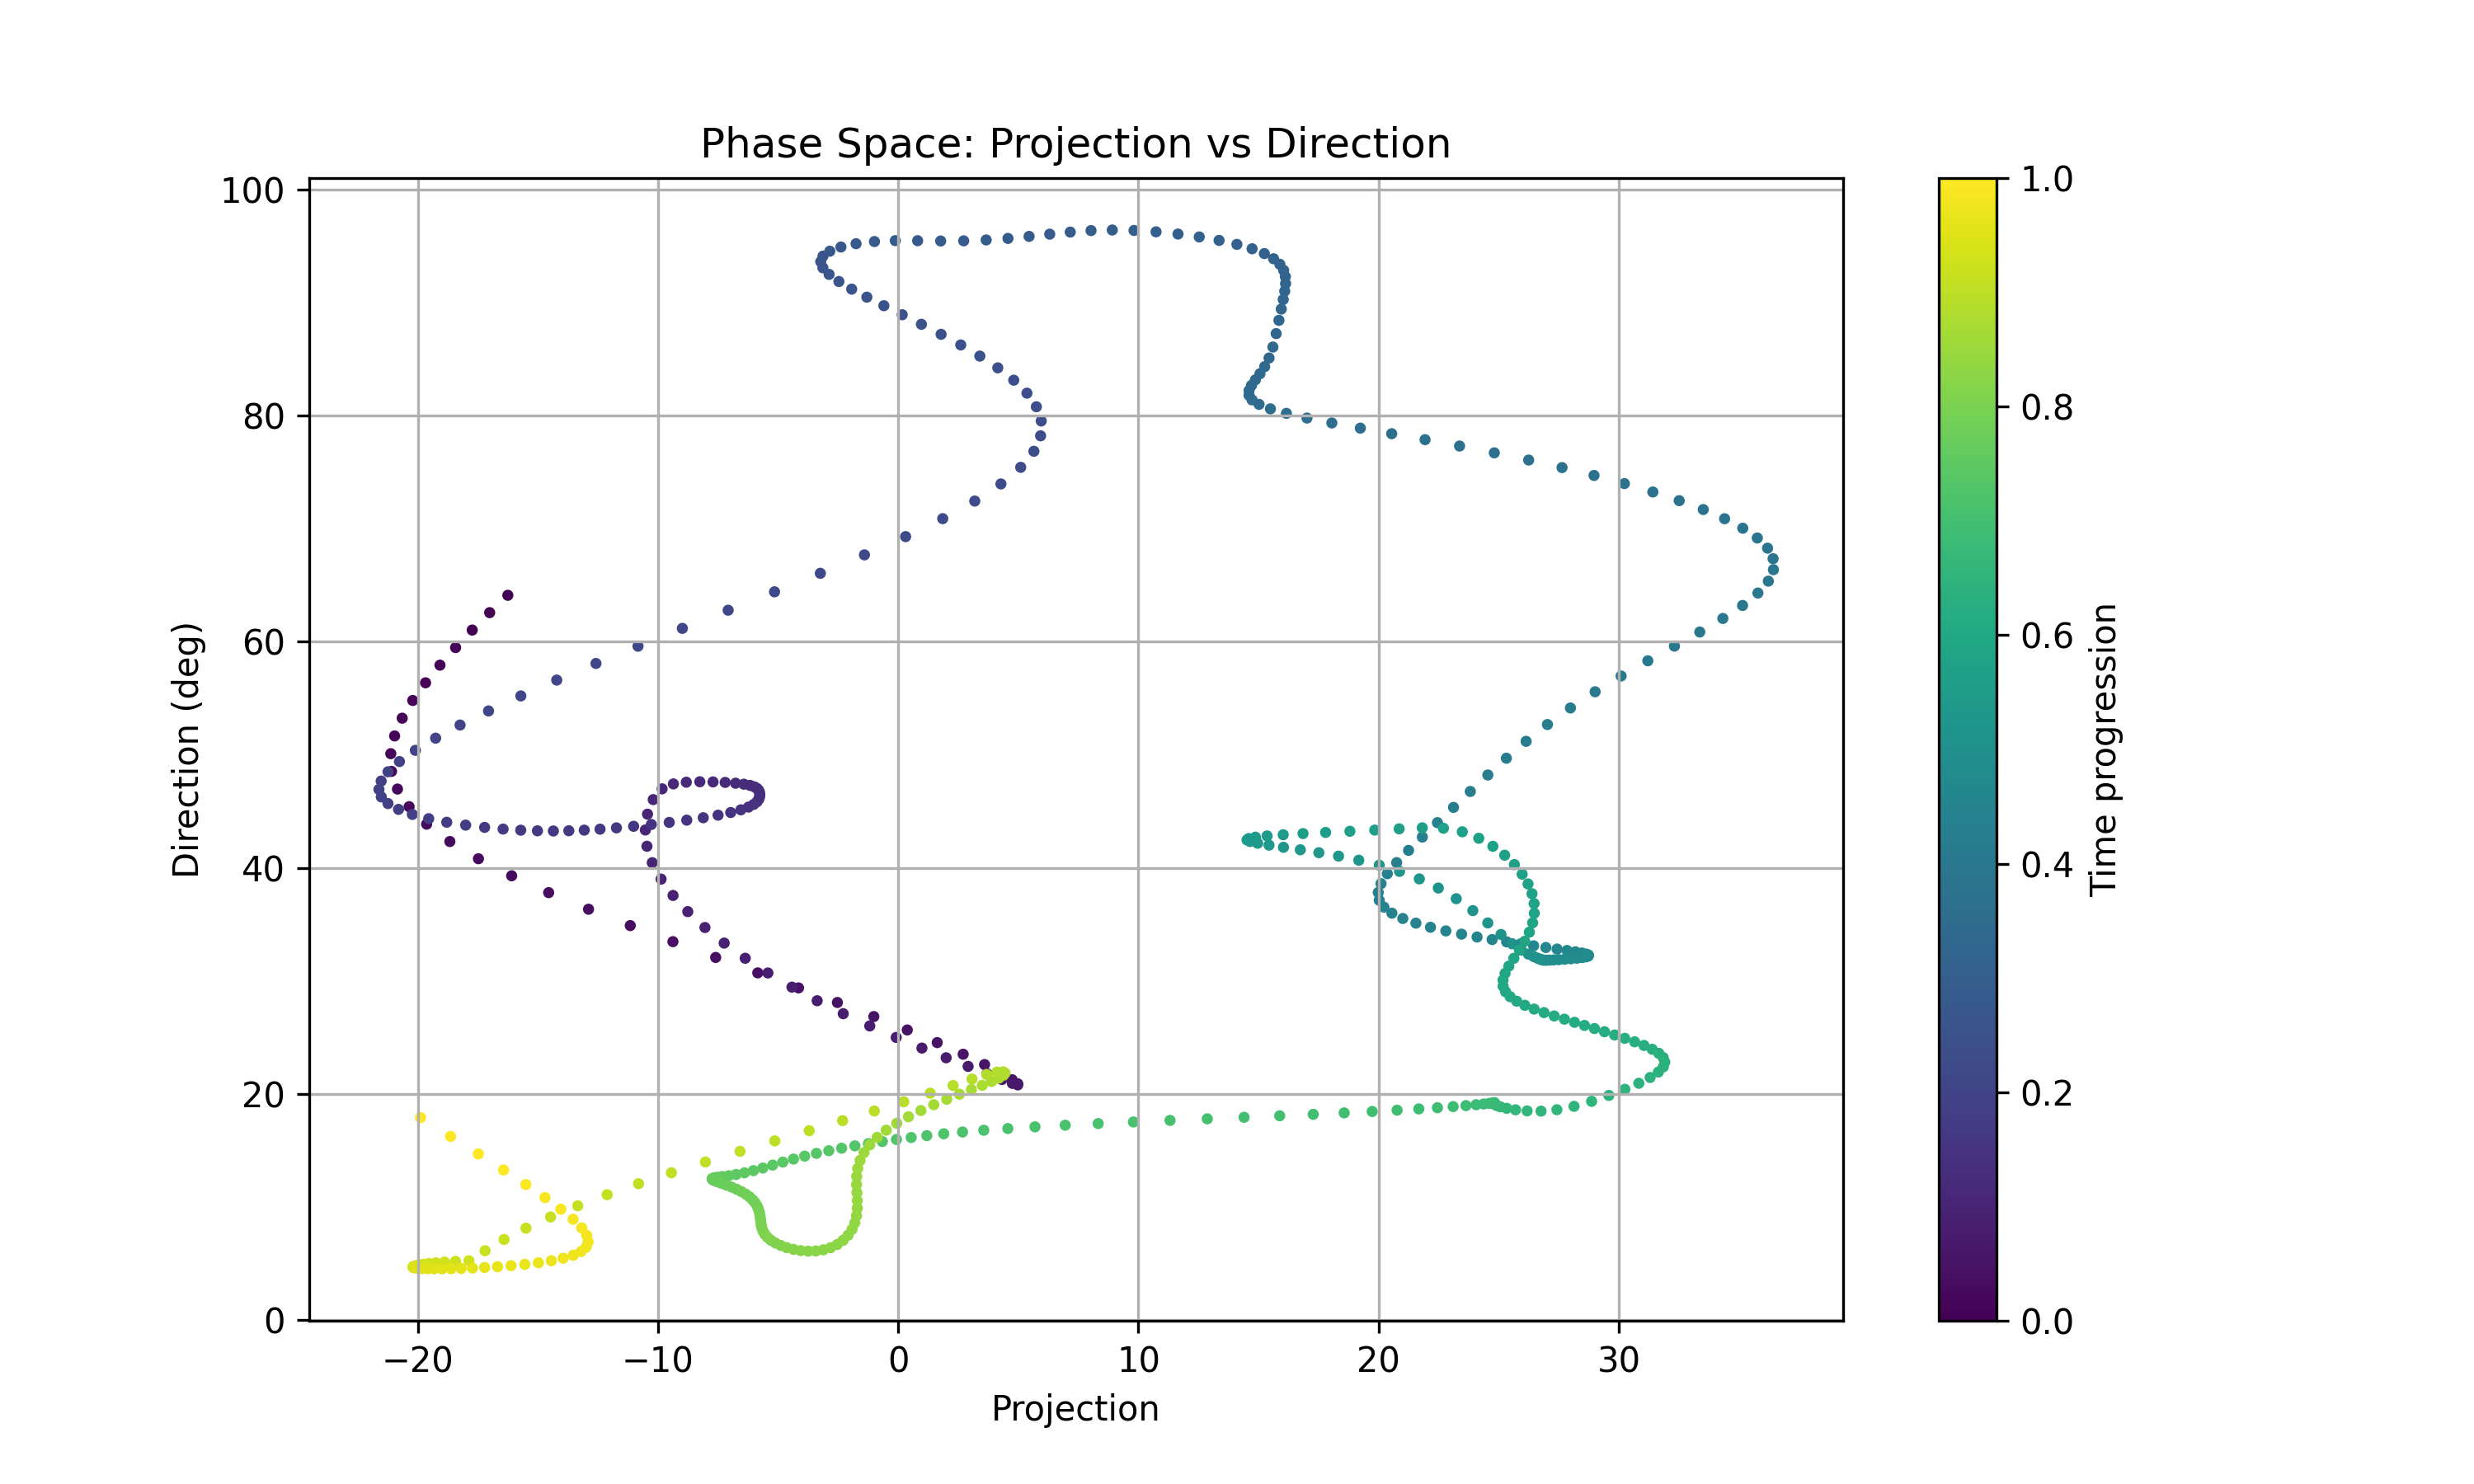
\includegraphics[width=0.5\textwidth]{fig_08_phase_space_projection.png}
\caption{Projected phase-space trajectory showing structured looping behavior.}
\label{fig:phase_projection}
\end{figure}

\subsection{Drift and Effective Potential}
\label{subsec:drift_and_effective_potential}

The conditional drift function $f(\theta) = \langle \dot{\theta} | \theta \rangle$ exhibits structured dependence on phase (Figure~\ref{fig:drift_function}).

\begin{figure}[h!]
\centering
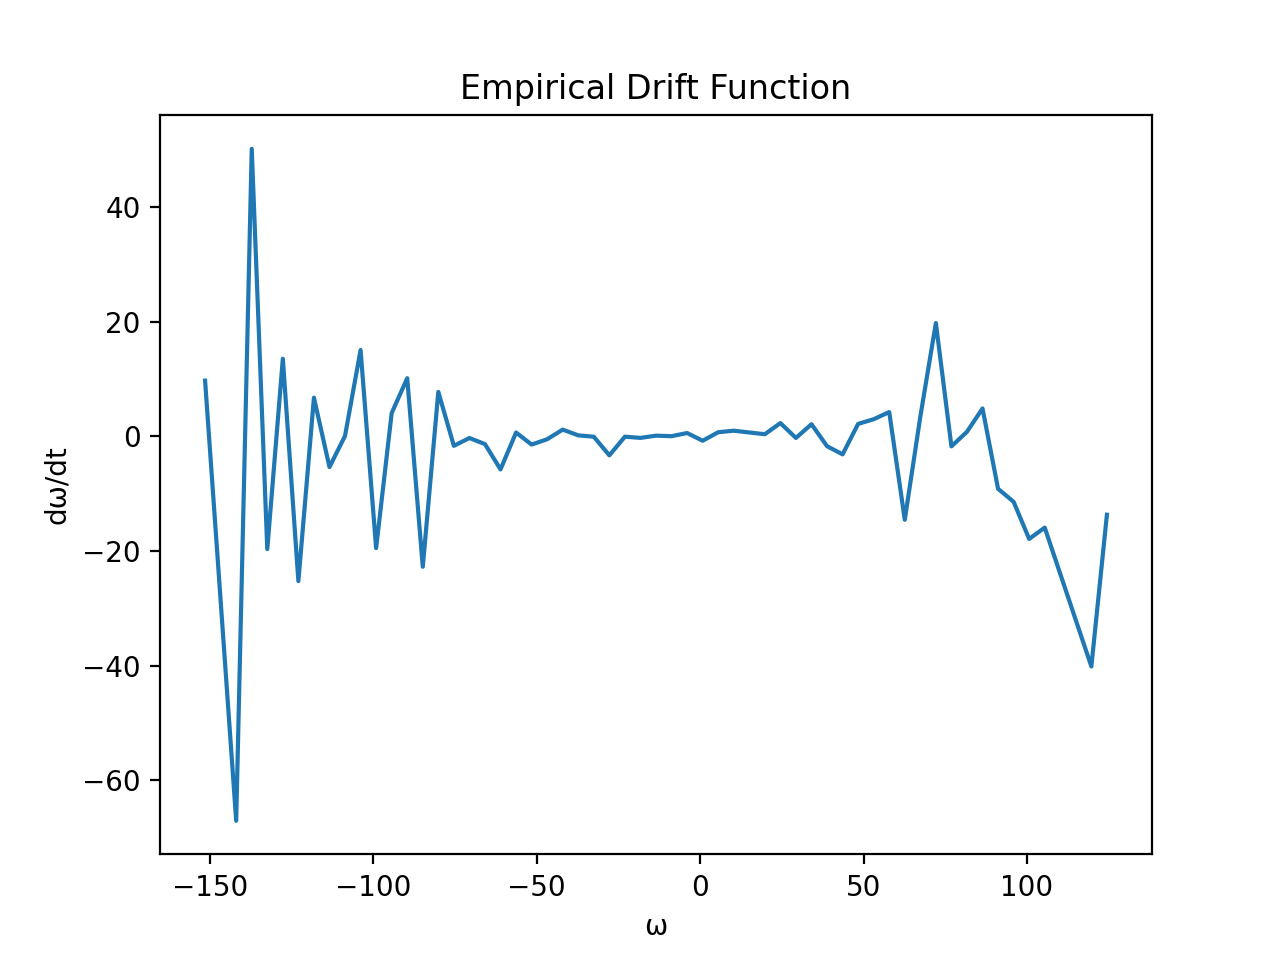
\includegraphics[width=0.5\textwidth]{fig_26_drift_function.png}
\caption{Estimated drift function showing state-dependent dynamics.}
\label{fig:drift_function}
\end{figure}

Integration of the drift yields an effective potential (Figure~\ref{fig:potential}), which suggests a bimodal structure, though the separation of wells is shallow and should be interpreted cautiously.

\begin{figure}[h!]
\centering
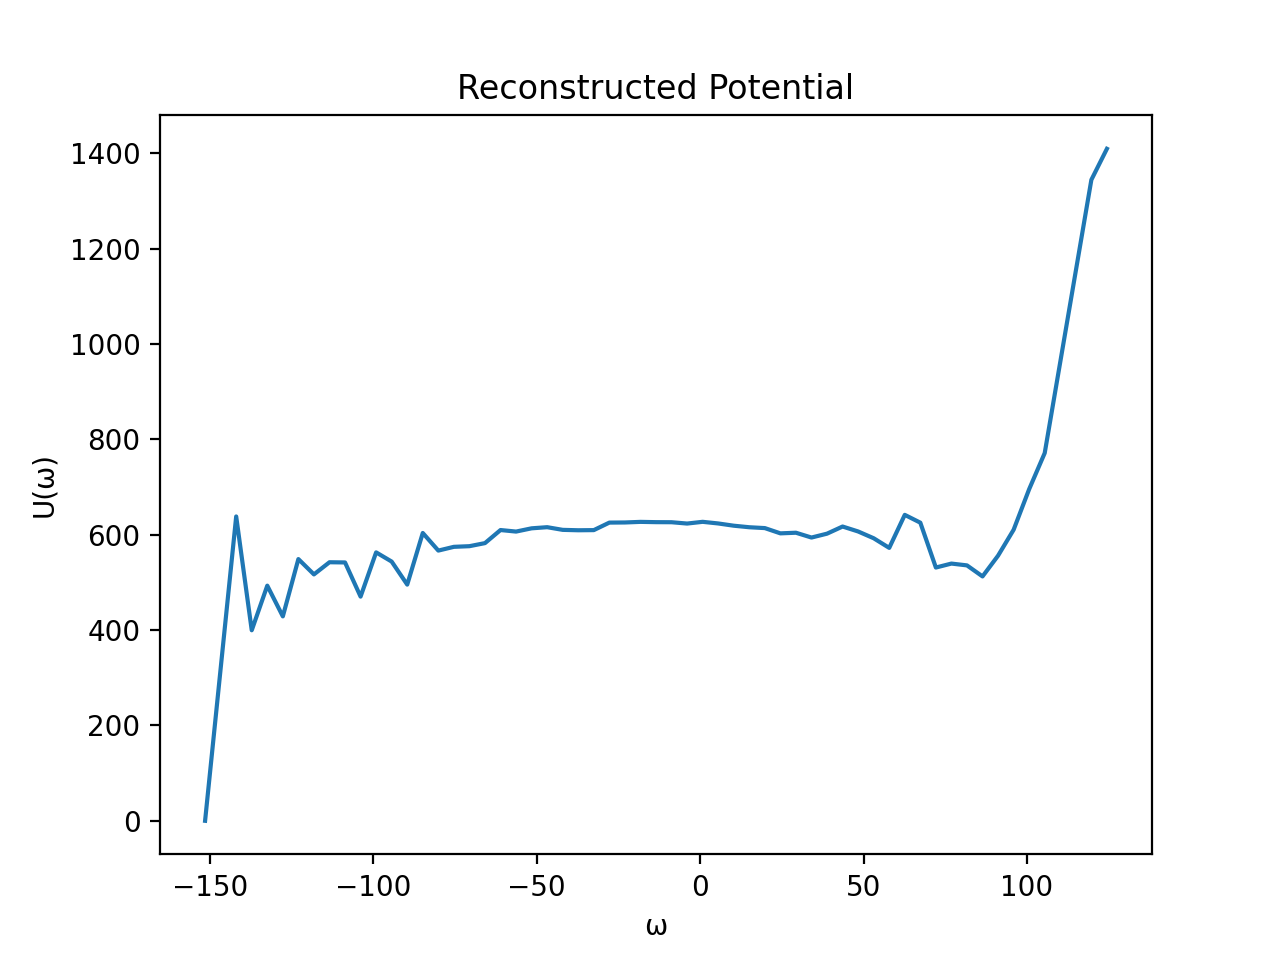
\includegraphics[width=0.5\textwidth]{fig_27_potential.png}
\caption{Reconstructed effective potential showing two metastable regions.}
\label{fig:potential}
\end{figure}

A two-dimensional representation of the potential (Figure~\ref{fig:potential_2d}) shows separation of regions corresponding to the two states.

\begin{figure}[h!]
\centering
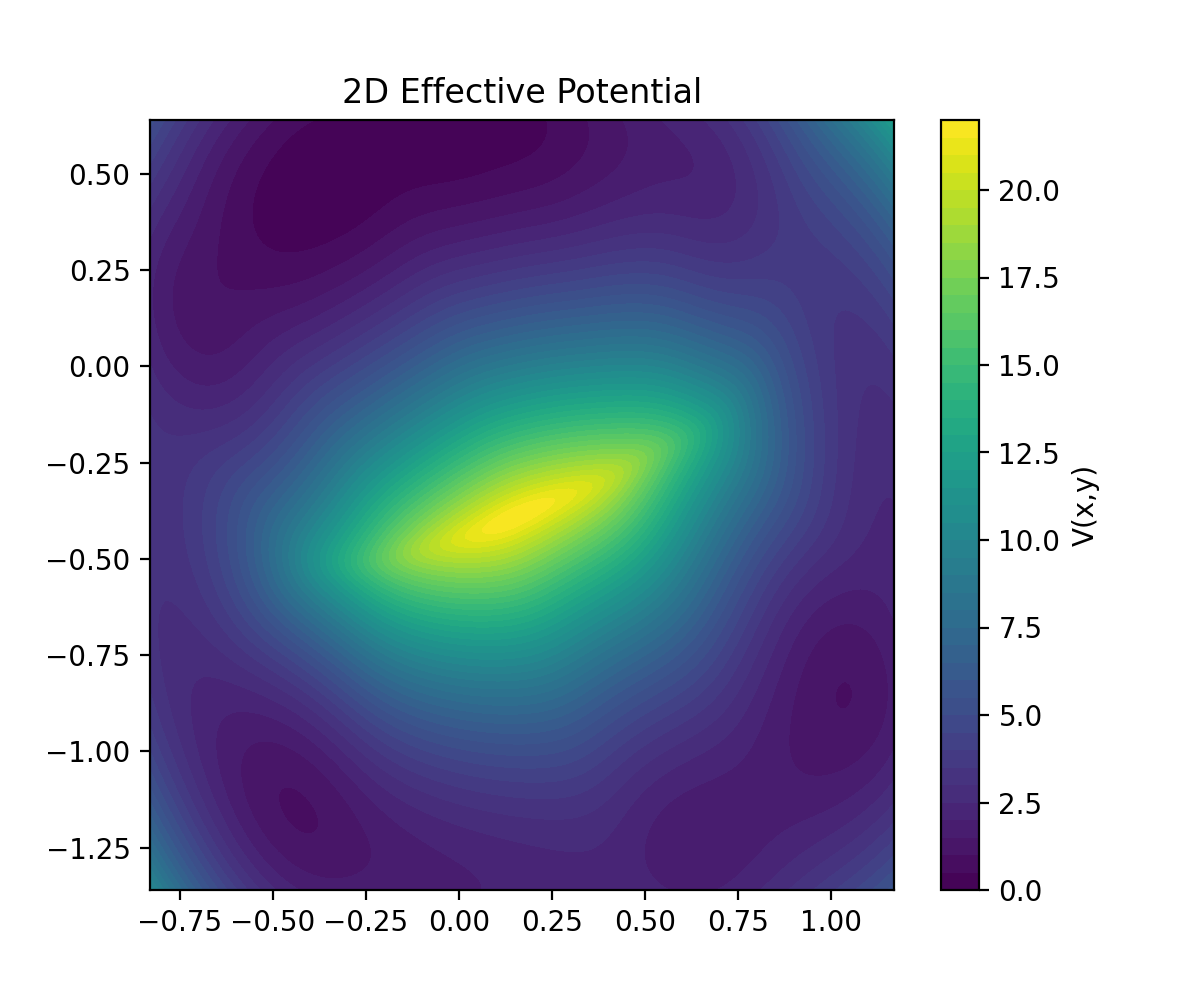
\includegraphics[width=0.5\textwidth]{fig_64_potential_2D.png}
\caption{Two-dimensional potential structure showing separation of metastable regions.}
\label{fig:potential_2d}
\end{figure}

\subsection{Interpretation of Dynamical Structure}
\label{subsec:interpretation_of_dynamical_structure}

The combined observations indicate:

\begin{itemize}
    \item Intermittent, burst-like transitions in angular velocity,
    \item Structured, non-diffusive trajectories in phase space,
    \item A bistable phenomenology consistent with, but not uniquely diagnostic of, a double-well potential.
\end{itemize}

These features are consistent with a system evolving on a constrained manifold with noise-driven transitions between metastable configurations.

Importantly, while the phase-space structure suggests coupling between degrees of freedom, no specific dynamical model is imposed at this stage. The results are interpreted as evidence of organized dynamics within a low-dimensional geometric framework, rather than as proof of a specific attractor topology.

\subsection{Summary of Dynamical Features}
\label{subsec:summary_of_dynamical_features}

The dynamical analysis supports the following conclusions:

\begin{enumerate}
    \item The system exhibits structured, non-diffusive dynamics with intermittent bursts,
    \item Phase-space trajectories are confined to a restricted region, indicating low-dimensional organization,
    \item The effective potential exhibits a double-well structure corresponding to two metastable states.
\end{enumerate}

Together with the geometric results of the previous section, this establishes a coherent picture of a bistable dynamical system evolving within a constrained geometric state space.

\subsection{SO(3) Reconstruction and Planar Constraint}
\label{subsec:so_3_reconstruction_and_planar_constraint}

The filtered trajectory is embedded in $\mathbb{R}^3$ as:
\begin{equation}
\mathbf{r}(t) = (x_f(t), y_f(t), z(t))
\end{equation}
with:
\begin{equation}
z(t) = \sqrt{1 - x_f^2(t) - y_f^2(t)}
\end{equation}

Empirically, $z(t) \approx 0$, indicating near-planar degeneracy.

To examine rotational structure, the trajectory is mapped into $\mathrm{SO}(3)$ using incremental rotations:
\begin{equation}
R(t + \Delta t) = \exp([\omega(t)]_\times \Delta t)\, R(t)
\end{equation}

The resulting trajectory (Figure~\ref{fig:so3_plane}) shows strong confinement to a single plane.

\begin{figure}[h!]
\centering
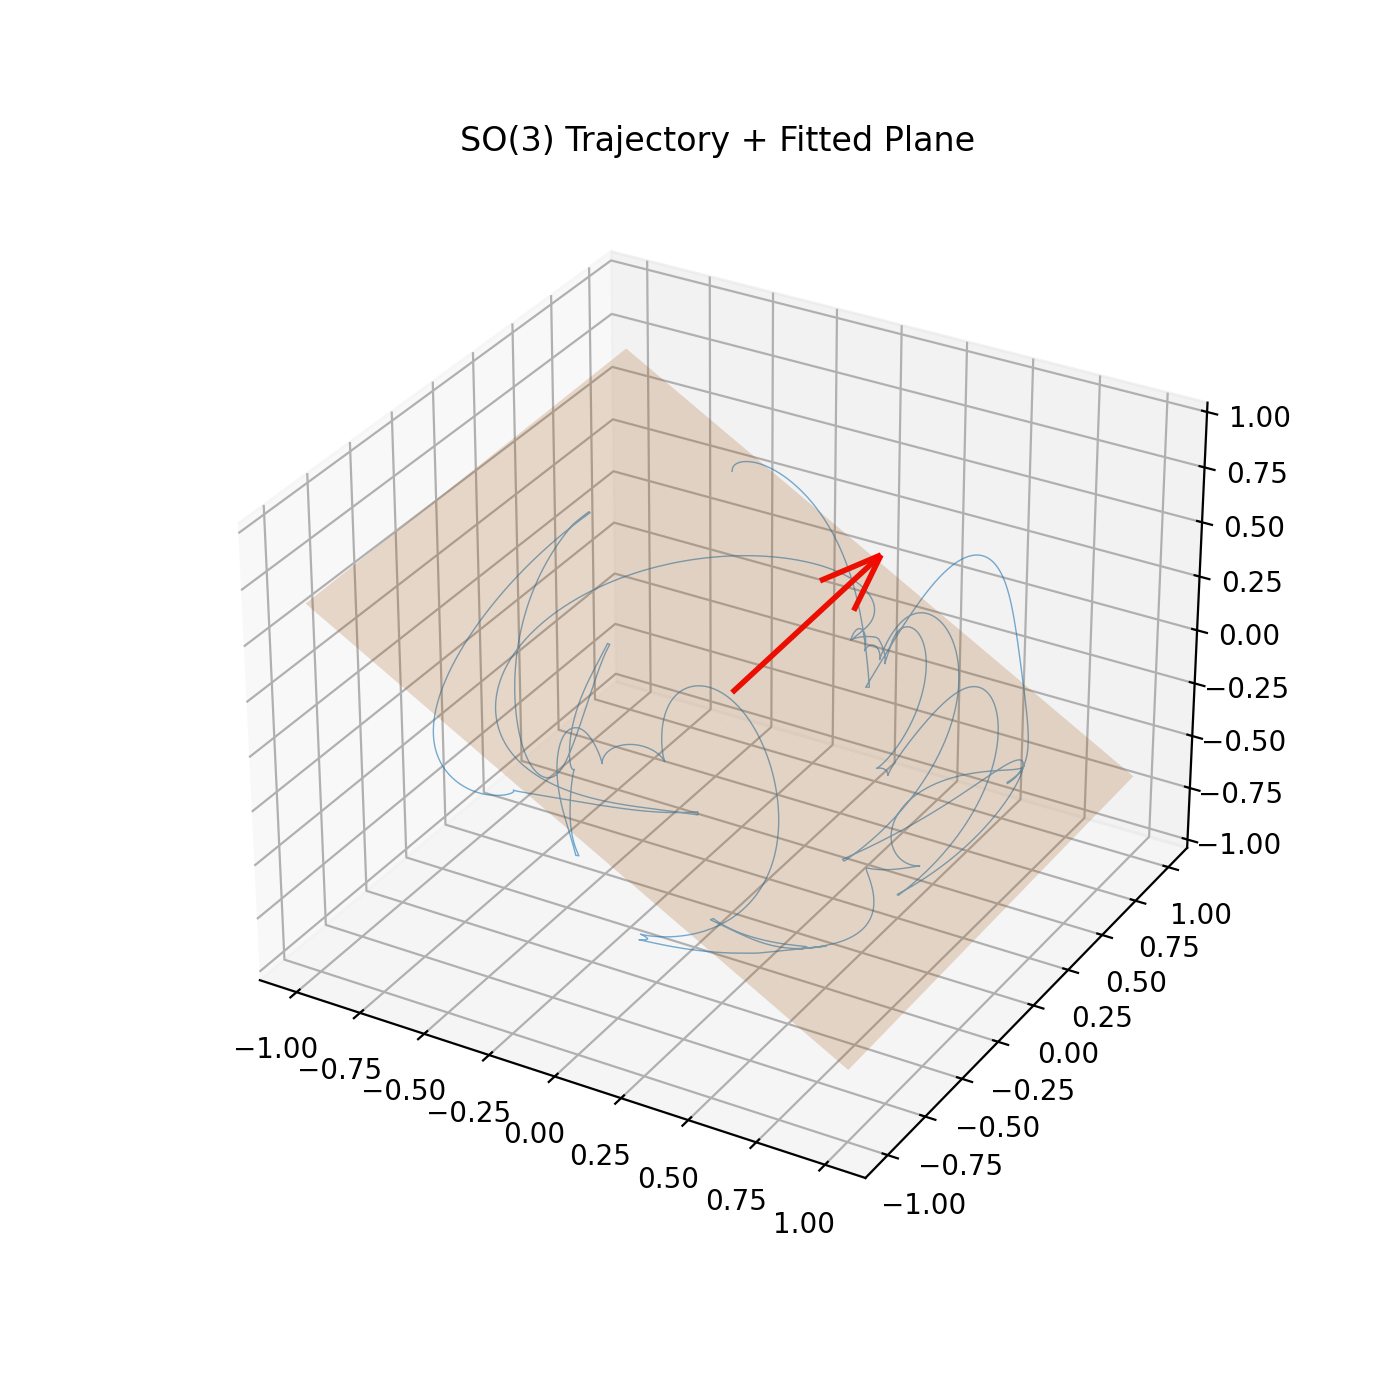
\includegraphics[width=0.5\textwidth]{fig_52_so3_plane.png}
\caption{Trajectory embedded in $\mathrm{SO}(3)$ showing confinement to a planar structure.}
\label{fig:so3_plane}
\end{figure}

\subsection{Intrinsic Plane Extraction}
\label{subsec:intrinsic_plane_extraction}

The intrinsic plane is extracted via covariance analysis in $\mathbb{R}^3$:
\begin{equation}
C = \langle \mathbf{r}(t)\mathbf{r}(t)^\top \rangle
\end{equation}

The plane normal is defined as the eigenvector corresponding to the smallest eigenvalue:
\begin{equation}
\mathbf{n} = \arg \min_{\|\mathbf{v}\|=1} \mathbf{v}^\top C \mathbf{v}
\end{equation}

The extracted plane is shown in Figure~\ref{fig:intrinsic_plane}.

\begin{figure}[h!]
\centering
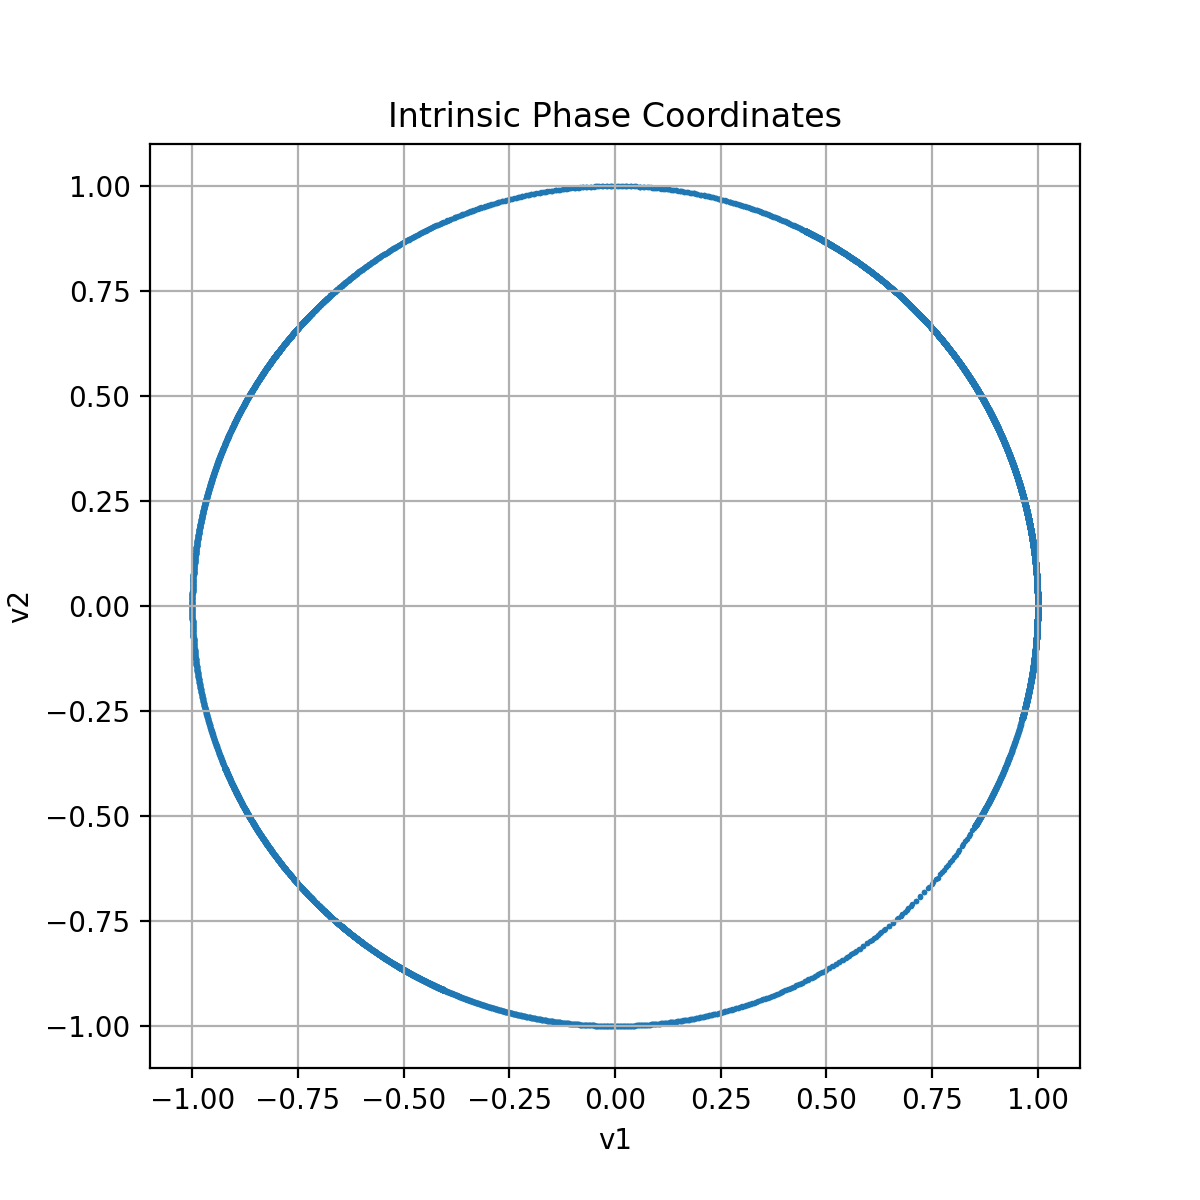
\includegraphics[width=0.5\textwidth]{fig_53_plane_intrinsic.png}
\caption{Intrinsic plane extracted from the trajectory, consistent with strong planar confinement.}
\label{fig:intrinsic_plane}
\end{figure}

This confirms that the planar structure is not an artefact of projection, but an intrinsic geometric property of the trajectory.

\subsection{Temporal Stability of the Axis}
\label{subsec:temporal_stability_of_the_axis}

The temporal evolution of the principal axis orientation is shown in Figure~\ref{fig:axis_time}.

\begin{figure}[h!]
\centering
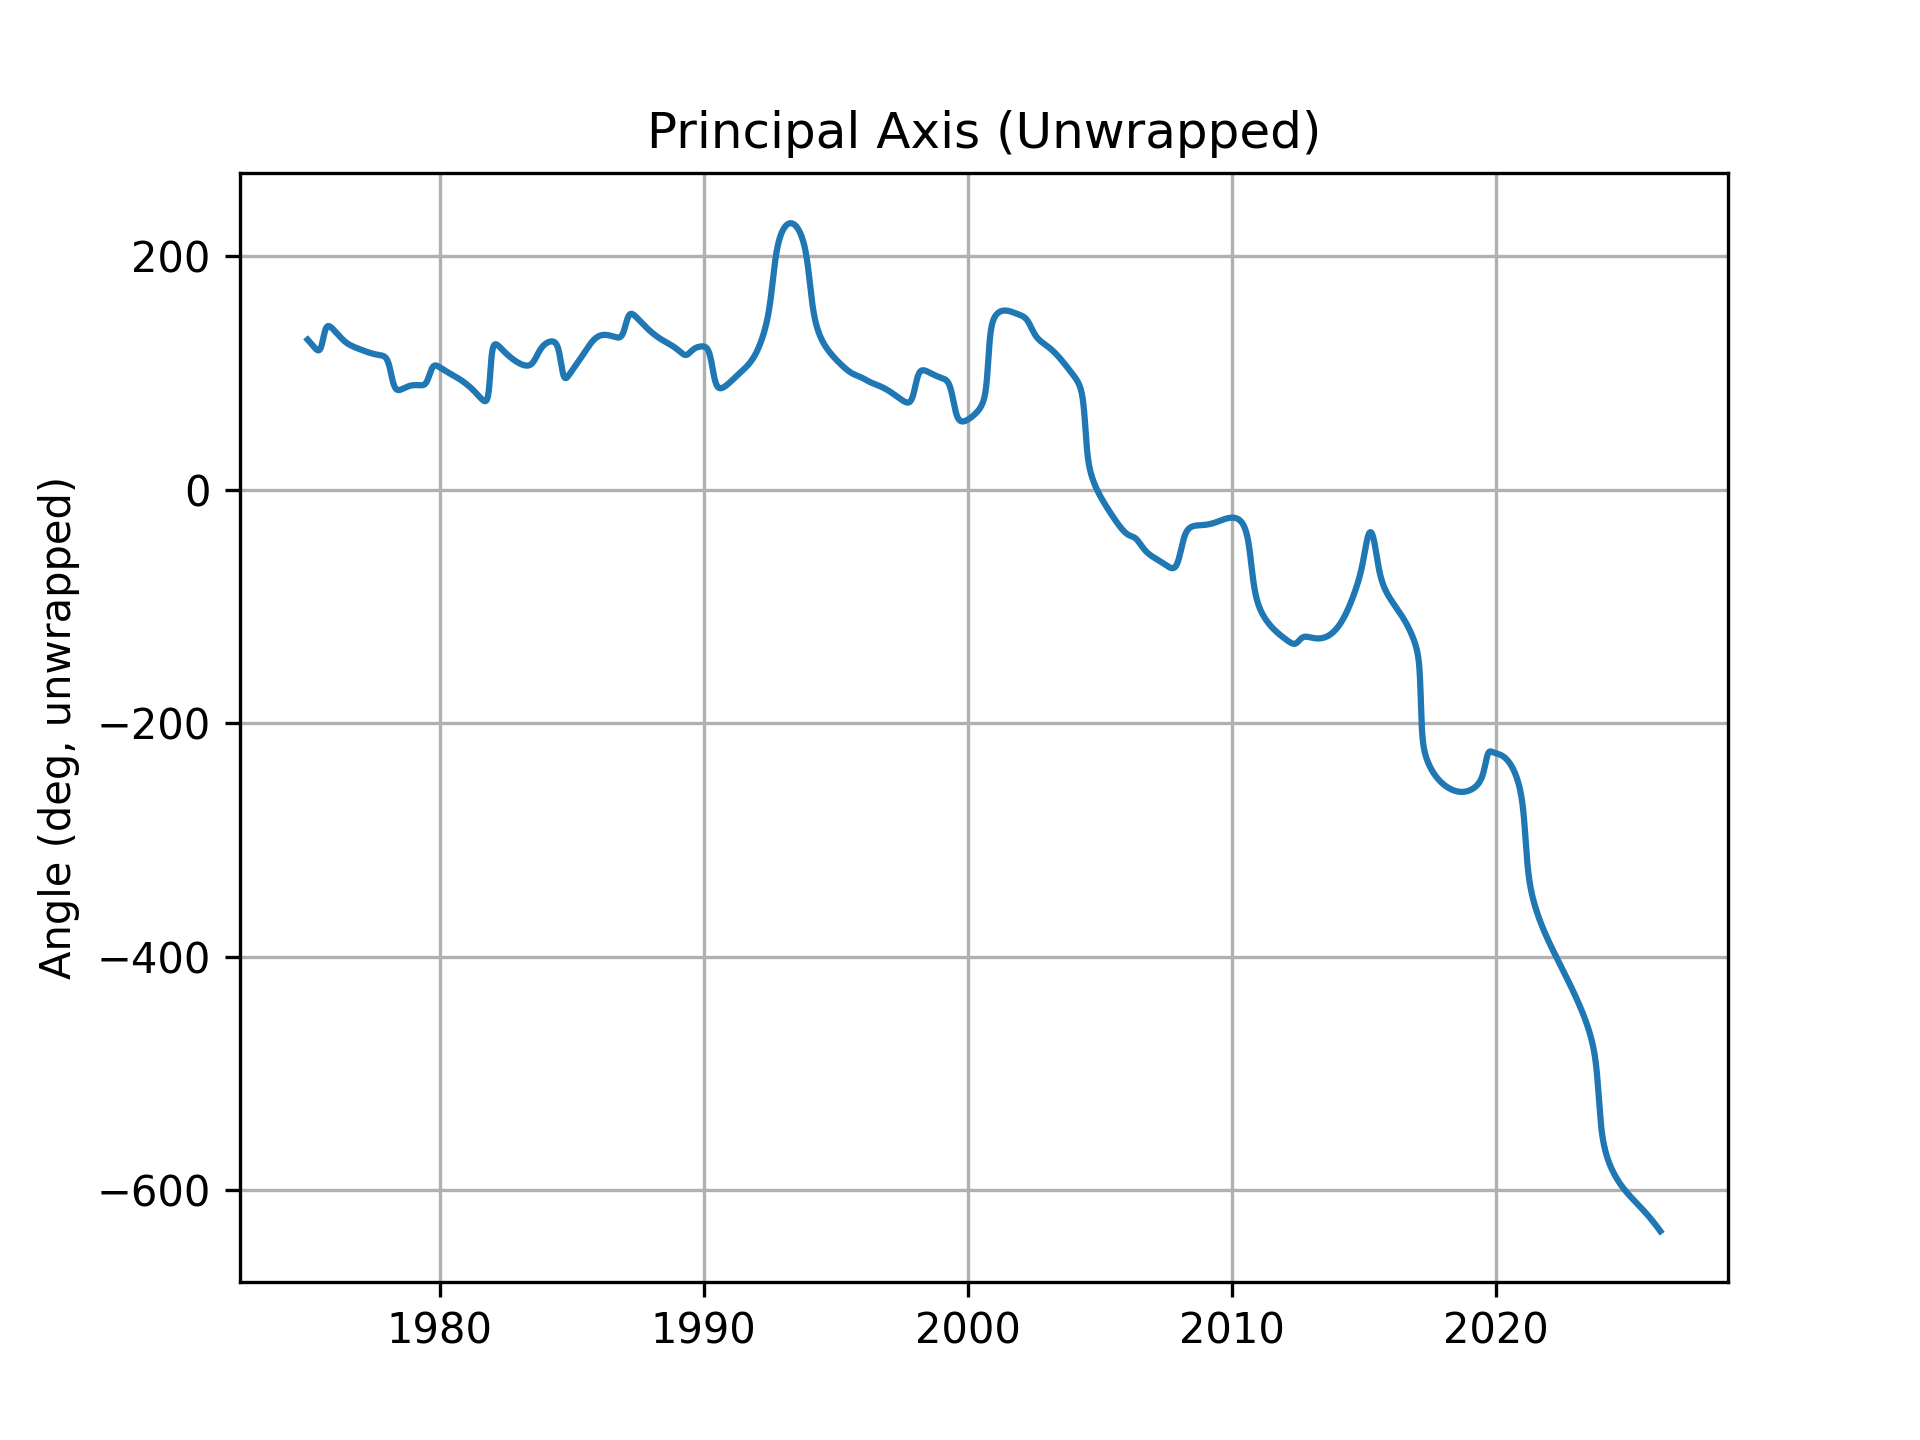
\includegraphics[width=0.5\textwidth]{fig_16_principal_axis_unwrapped.png}
\caption{Temporal evolution of the principal axis orientation (unwrapped angle).}
\label{fig:axis_time}
\end{figure}

The axis exhibits relatively small fluctuations over time, suggesting apparent stability over the observation window.

\subsection{Axis Stability Under Null Models}
\label{subsec:axis_stability_under_null_models}

To assess whether this apparent stability reflects a genuine constraint, a rotational null model is applied in which the trajectory is randomly rotated at each time step.

The variability of the axis under this null model is statistically indistinguishable from that of the observed data. This indicates that the observed axis stability does not exceed what is expected from randomized rotational baselines.

Accordingly, the axis should be interpreted as a consistent geometric feature of the trajectory, but not as statistically confirmed evidence of an externally fixed orientation.

\subsection{Axis Geometry and Deviation}
\label{subsec:axis_geometry_and_deviation}

Deviation from the principal axis is defined as:
\begin{equation}
d(t) = \arccos(\mathbf{x}(t) \cdot \mathbf{a})
\end{equation}

The deviation remains bounded over time (Figure~\ref{fig:axis_deviation}), indicating persistent alignment with the dominant direction.

\begin{figure}[h!]
\centering
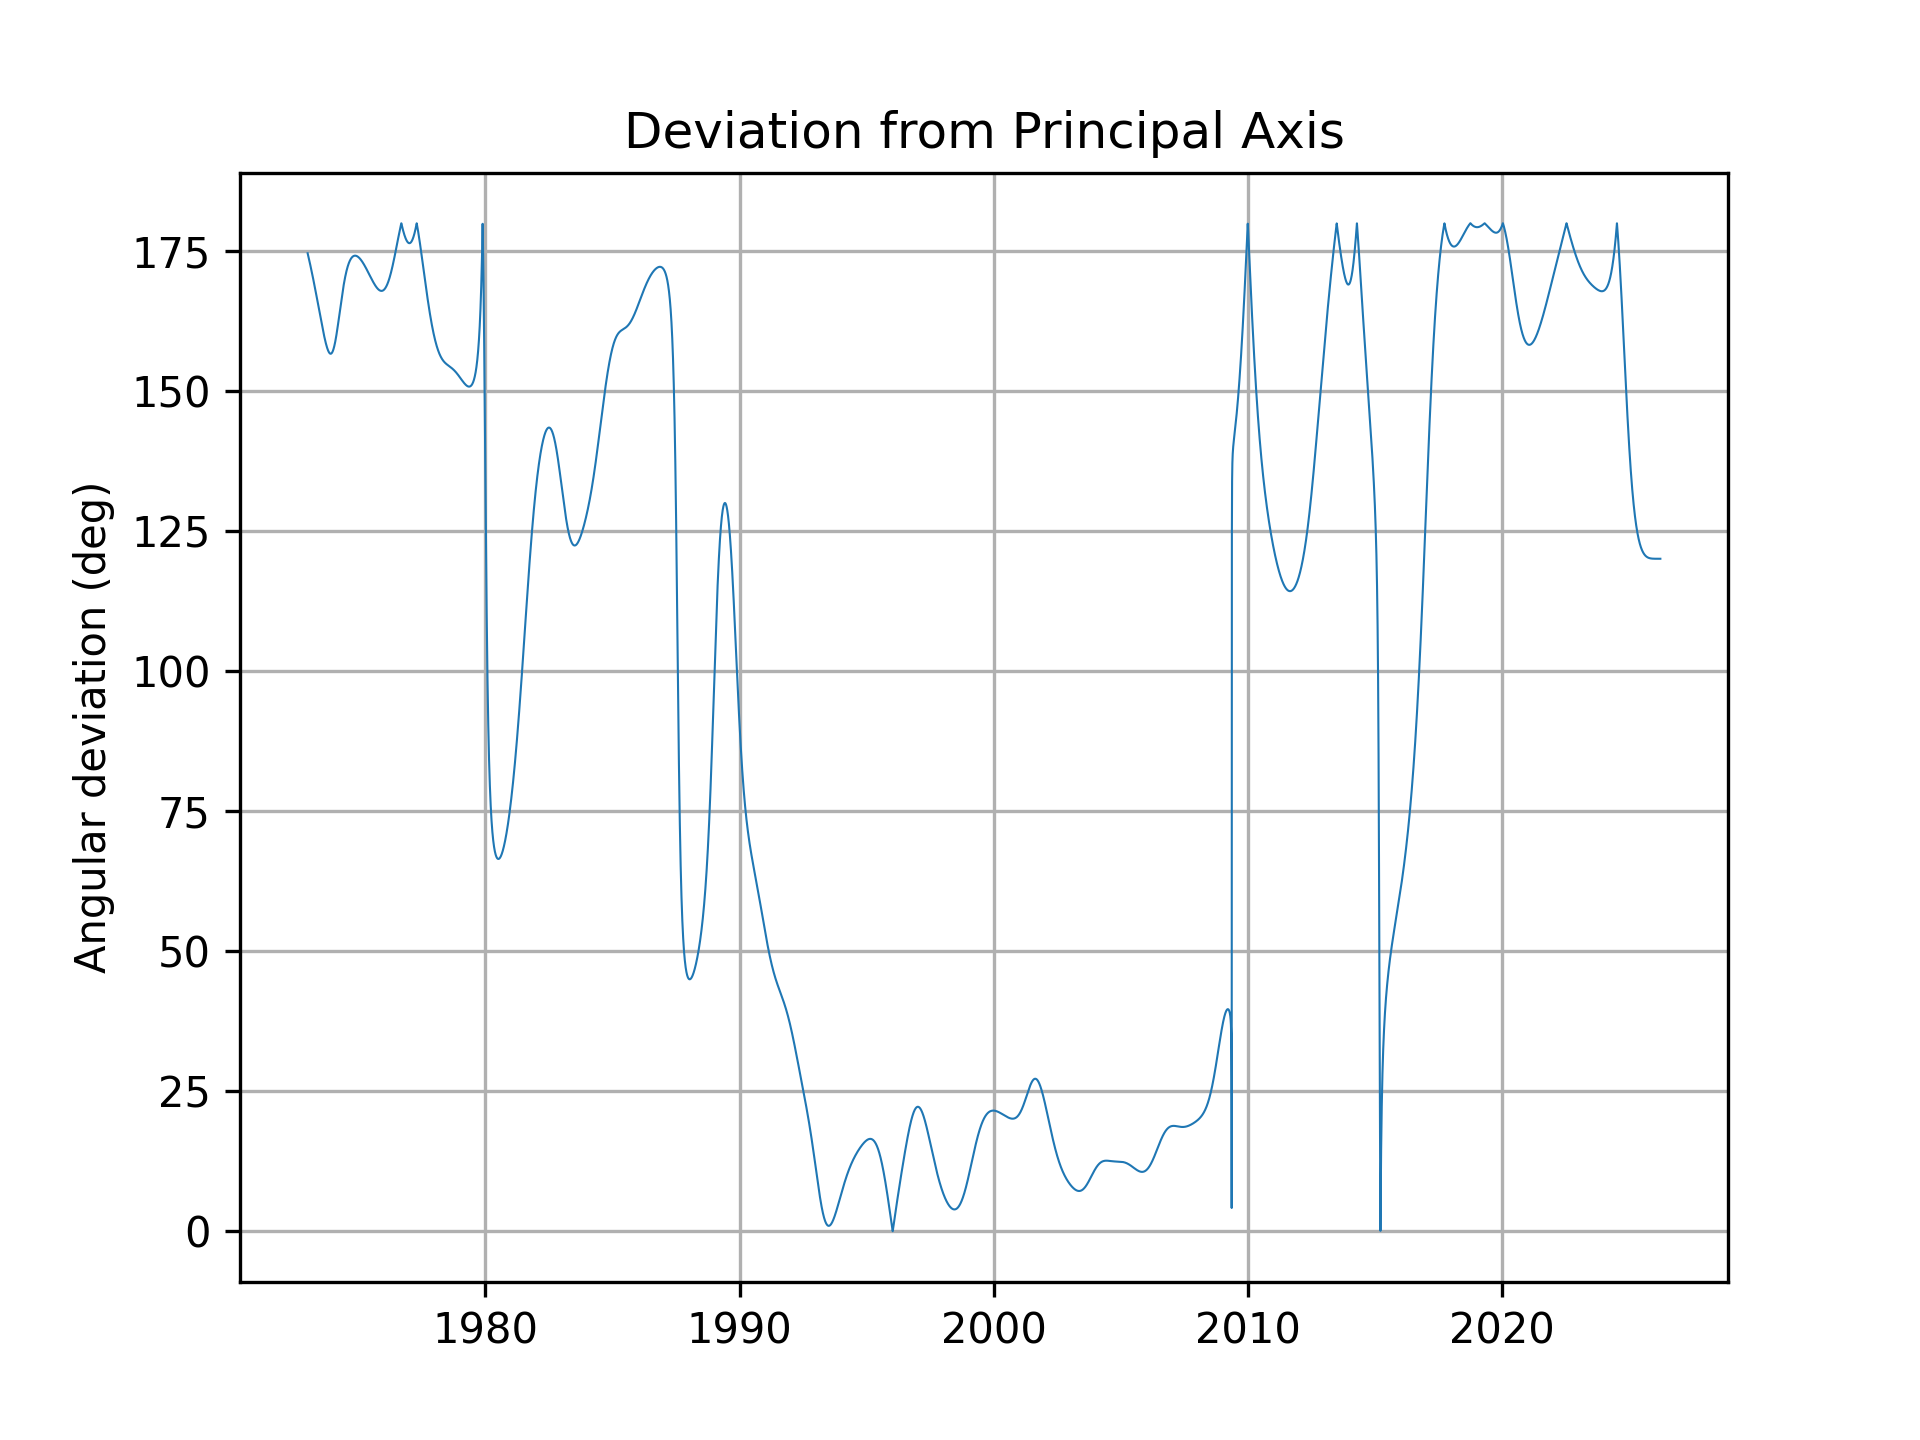
\includegraphics[width=0.5\textwidth]{fig_10_axis_deviation.png}
\caption{Angular deviation from the dominant axis showing bounded variation.}
\label{fig:axis_deviation}
\end{figure}

\subsection{Interpretation of Axis Geometry}
\label{subsec:interpretation_of_axis_geometry}

The results of this section establish:

\begin{itemize}
    \item Strong confinement of the trajectory to a planar manifold,
    \item A well-defined principal axis organizing the motion,
    \item Bounded deviation from this axis over time.
\end{itemize}

However, robustness testing shows that the apparent temporal stability of the axis is not statistically distinguishable from that produced by randomized rotational processes.

This leads to a refined interpretation:

\begin{quote}
The principal axis represents a consistent geometric feature of the trajectory, but its apparent stability does not, by itself, constitute evidence of a fixed external reference frame.
\end{quote}

\subsection{Full-Sphere Directional Analysis}
\label{subsec:full_sphere_directional_analysis}

Directional alignment is evaluated over the unit sphere by projecting velocity vectors onto candidate directions $\hat{\mathbf{g}}$:
\begin{equation}
E(\hat{\mathbf{g}}) = \sum_t \left( \mathbf{v}(t) \cdot \hat{\mathbf{g}} \right)^2
\end{equation}

The resulting distribution of directional alignment is shown in Figure~\ref{fig:anisotropy_distribution}.

\begin{figure}[h!]
\centering
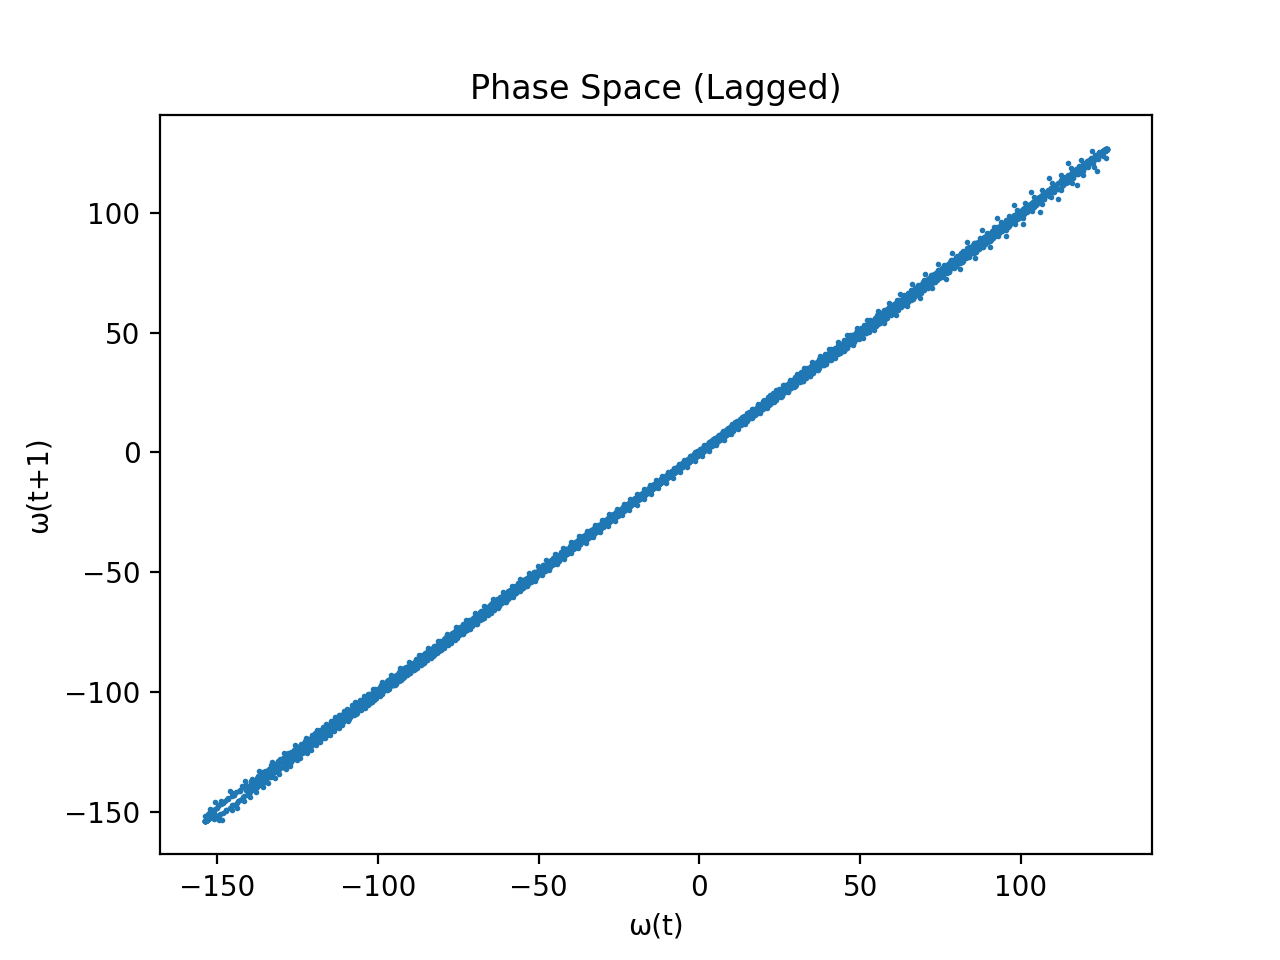
\includegraphics[width=0.5\textwidth]{fig_23_phase_space.png}
\caption{Directional alignment distribution relative to candidate axes.}
\label{fig:anisotropy_distribution}
\end{figure}

A preferred direction is identifiable geometrically as the maximum of $E(\hat{\mathbf{g}})$.

\subsection{Comparison with Surrogate Models}
\label{subsec:comparison_with_surrogate_models}

To assess statistical significance, the observed alignment distribution is compared with surrogate datasets.

When evaluated against colored-noise (AR(1)) surrogates, the magnitude of directional alignment does not exceed the surrogate distribution. The observed anisotropy falls within the expected range of correlated stochastic processes.

This indicates that while a preferred direction can be identified geometrically, its magnitude is not statistically distinguishable from that produced by temporally correlated noise.

\subsection{Phase-Space Dependence of Directionality}
\label{subsec:phase_space_dependence_of_directionality}

The relationship between directional alignment and system state is shown in Figure~\ref{fig:anisotropy_phase}.

\begin{figure}[h!]
\centering
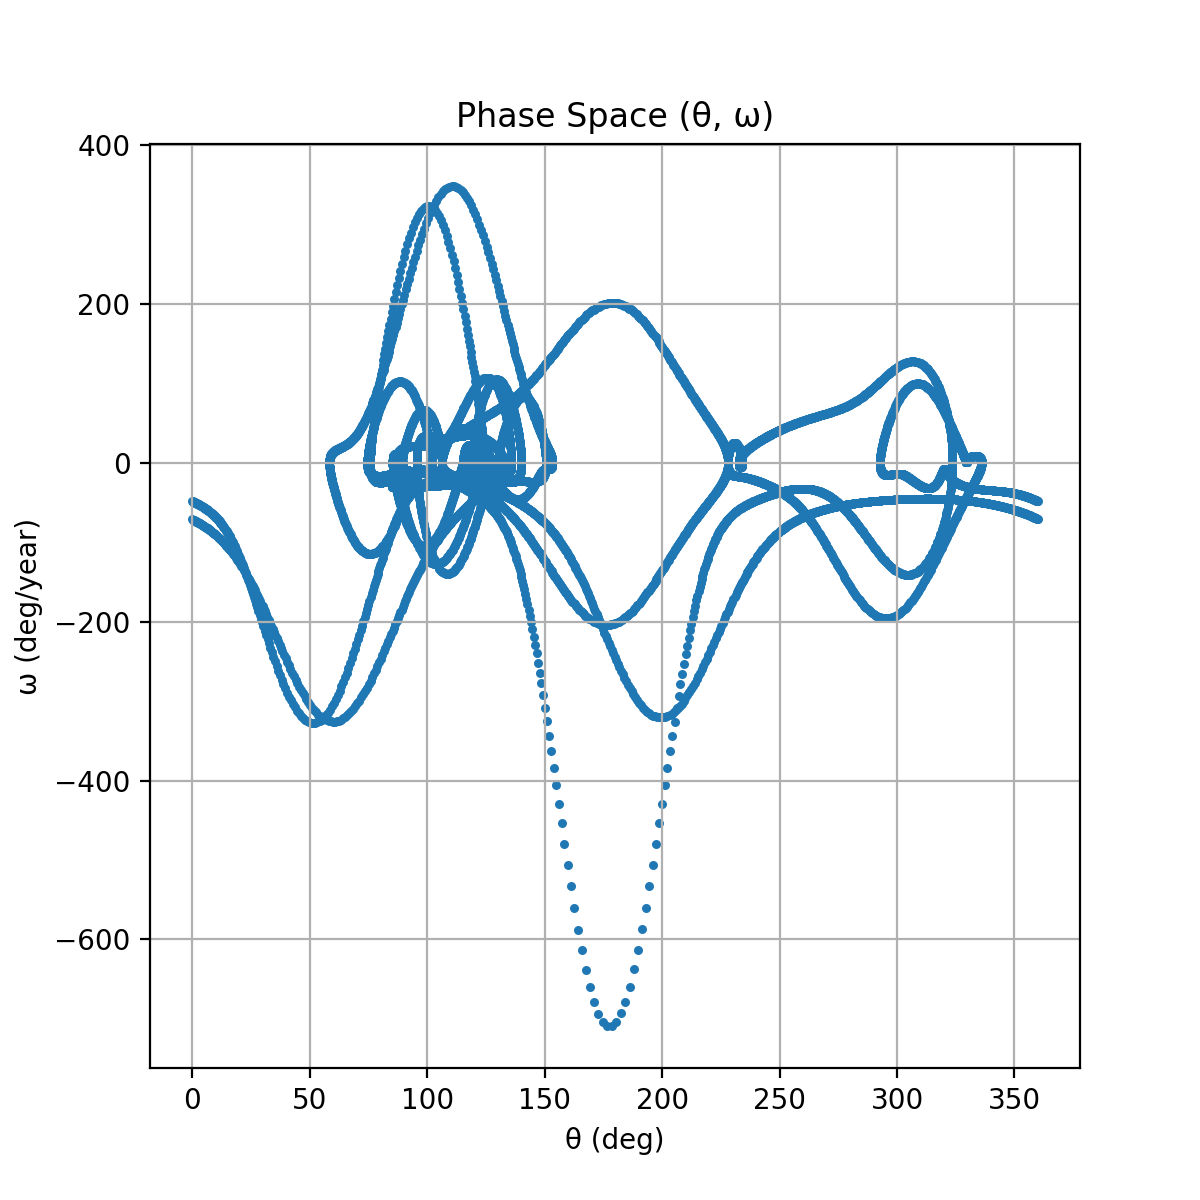
\includegraphics[width=0.5\textwidth]{fig_70_phase_space.png}
\caption{Phase-space relationship between directional alignment and system state.}
\label{fig:anisotropy_phase}
\end{figure}

Directional alignment evolves coherently with system state rather than appearing as independent random fluctuations. This indicates that directional structure is coupled to the internal dynamics of the system and is not fully captured by null models that disrupt phase continuity.

\subsection{Spherical Harmonic Decomposition}
\label{subsec:spherical_harmonic_decomposition}

The directional distribution is expanded in spherical harmonics:
\begin{equation}
f(\theta, \phi) = \sum_{\ell,m} a_{\ell m} Y_{\ell m}(\theta, \phi)
\end{equation}

The corresponding power spectrum is:
\begin{equation}
P_\ell = \sum_m |a_{\ell m}|^2
\end{equation}

Empirical results show:

\begin{itemize}
    \item Dipole power: $P_1 \ll 1$
    \item Quadrupole power: $P_2 \gg P_1$
\end{itemize}

indicating dominance of quadrupolar structure.

\subsection{Interpretation of Harmonic Structure}
\label{subsec:interpretation_of_harmonic_structure}

The dominance of quadrupole power implies that the directional structure is not a simple bias toward a single direction, but instead reflects a higher-order symmetry with opposing regions of alignment.

This is consistent with the observed two-state structure, in which the system alternates between opposing regions of phase space.

Importantly, the quadrupolar structure is a geometric property of the distribution and does not depend on the statistical significance of the anisotropy magnitude.

\subsection{Summary of Directional Structure}
\label{subsec:summary_of_directional_structure}

The results of this section establish:

\begin{enumerate}
    \item A geometrically identifiable preferred direction,
    \item Directional alignment that varies coherently with system state,
    \item A quadrupole-dominated angular structure.
\end{enumerate}

At the same time, the magnitude of absolute (Earth-fixed) anisotropy does not exceed that expected under correlated stochastic models, indicating that directional strength should not be interpreted as evidence of external forcing.

The directional structure is therefore best understood as an emergent feature of the system's internal dynamics within a constrained geometric state space.

\subsection{Planetary Torque Conditioning of High-Deviation States}

We now introduce an additional empirical constraint on the system: the distribution of
high-deviation states in the polar motion manifold is not uniform with respect to planetary
torque configuration.

To evaluate this, we define a planetary phase index constructed from the relative angular
configuration of major bodies. We then condition the occurrence of high $R(t)$ states
on this phase space and compare against phase-randomized null distributions, following the same general logic used in surrogate-based nonlinear time-series inference \citep{theiler1992,schreiber2000}.

\begin{figure}[h]
\centering
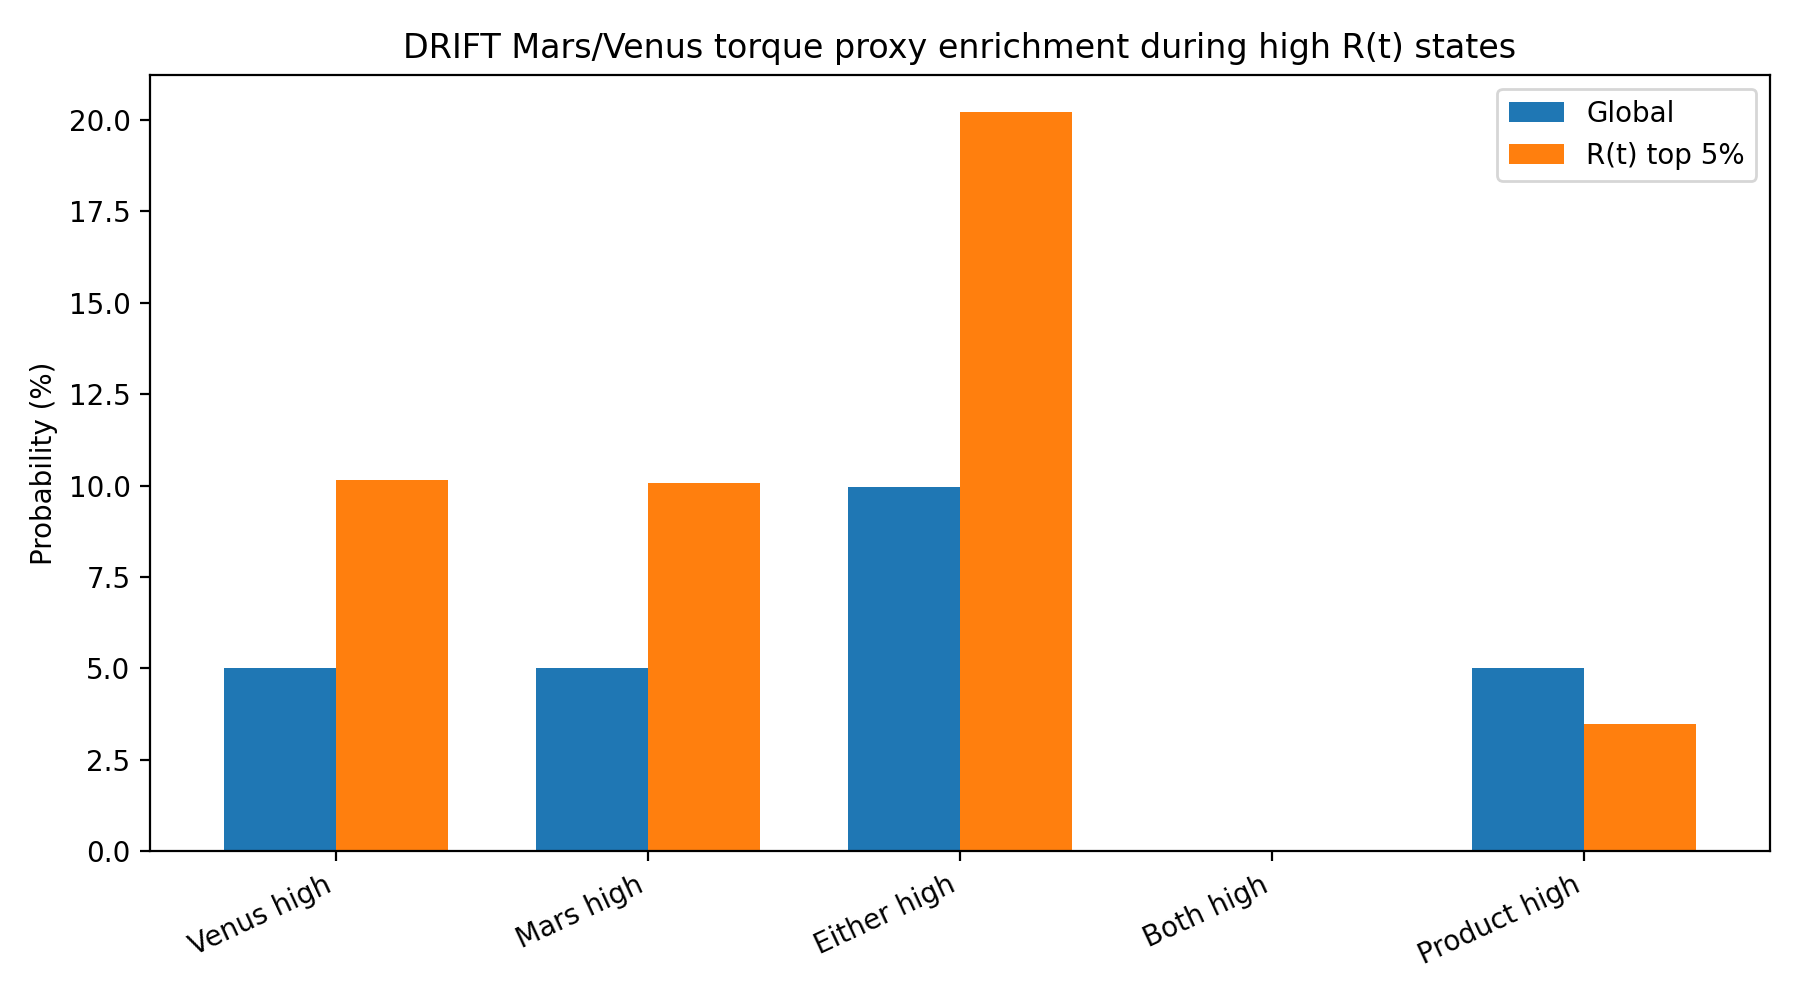
\includegraphics[width=0.48\textwidth]{outputs/drift_torque_conditioning_results/01_global_vs_Rhigh_enrichment.png}
\caption{
Global vs high-$R$ state enrichment across planetary phase space. High-deviation
rotational states are not uniformly distributed, but exhibit clear concentration
in specific phase sectors. This indicates that planetary configuration acts as a
conditioning variable on the rotational state of the Earth system, rather than a
continuous forcing term.
}
\label{fig:torque_enrichment}
\end{figure}

The enrichment structure is sharply localized, indicating that only a subset of phase
configurations contribute meaningfully to the occurrence of high-deviation states.
This immediately constrains any viable coupling mechanism: the effect must be phase-selective,
not broadband.

\subsection{Lagged Coherence Between Torque Phase and Rotational Response}

We next examine whether the relationship between planetary configuration and rotational
state exhibits a temporal structure.

A lagged correlation analysis reveals a non-symmetric response, with maximal coherence
occurring at finite positive lag. This indicates that the rotational system responds
to planetary phase configuration with a measurable delay.

\begin{figure}[h]
\centering
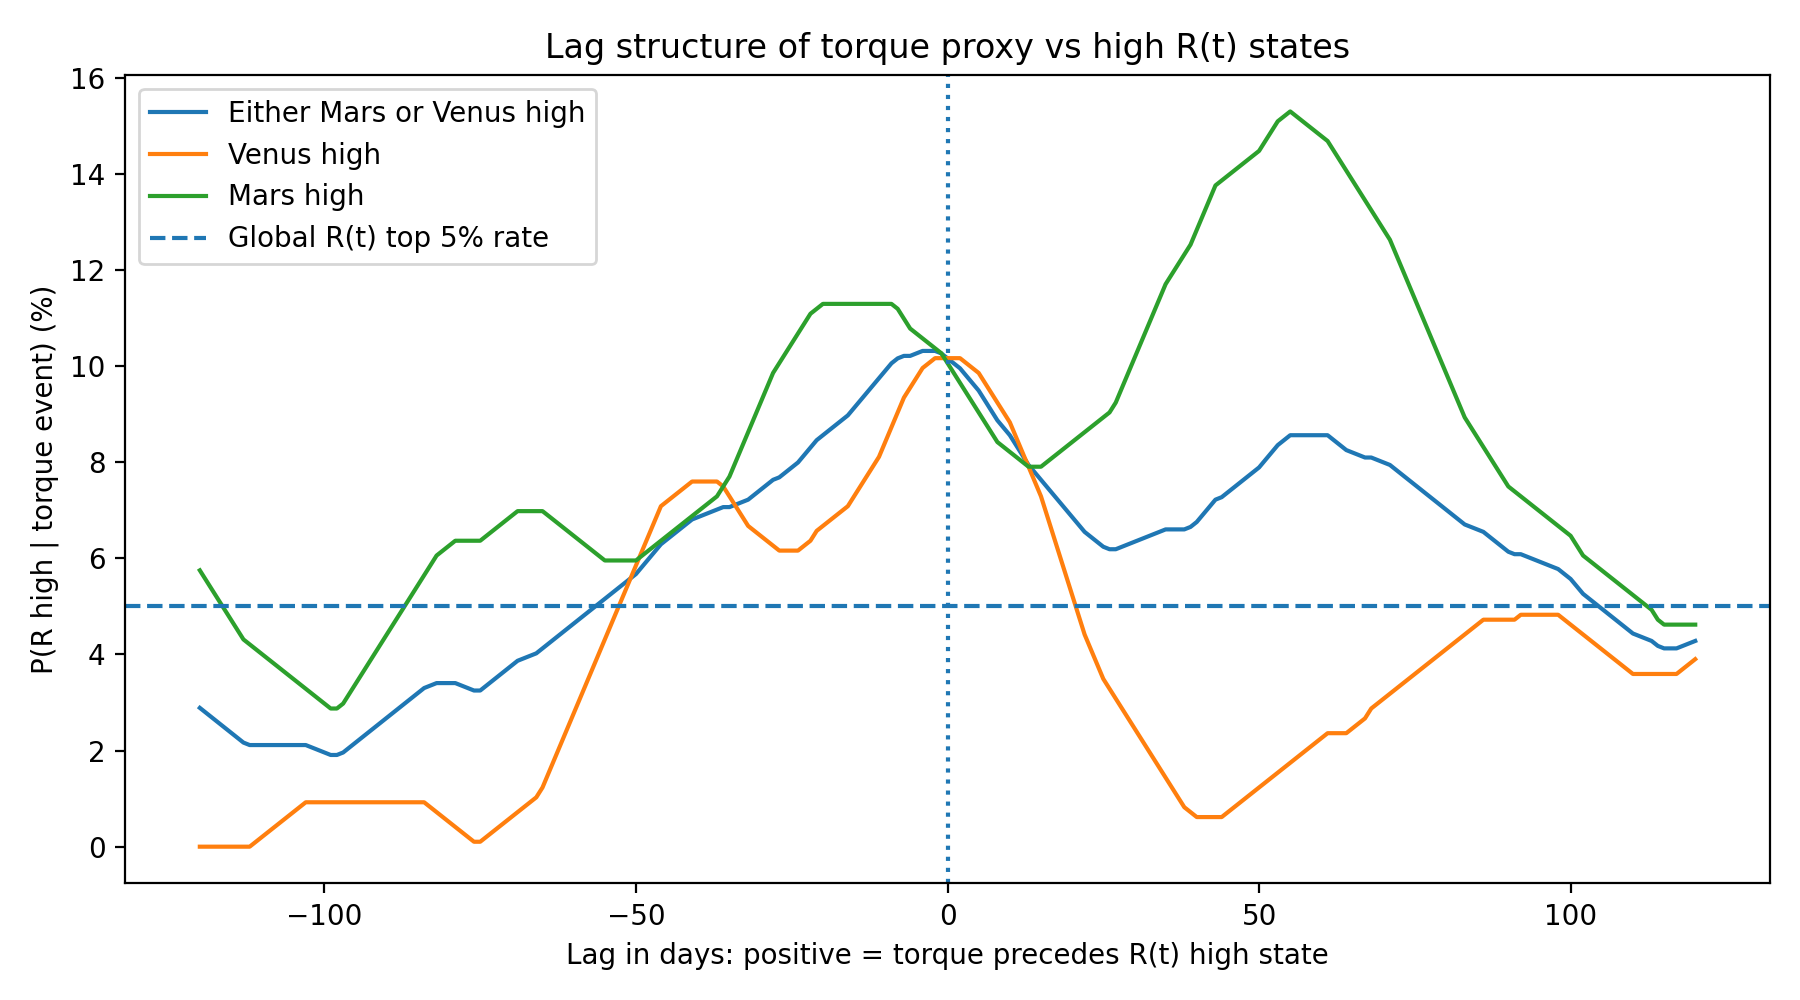
\includegraphics[width=0.48\textwidth]{outputs/drift_torque_conditioning_results/02_lag_probability.png}
\caption{
Lag-dependent probability of high-deviation states conditioned on planetary phase.
The peak at positive lag indicates that planetary configuration precedes the
rotational response, consistent with a causal but indirect modulation mechanism.
}
\label{fig:lag_probability}
\end{figure}

The presence of a preferred lag is inconsistent with instantaneous forcing, and instead
supports an interpretation in which planetary geometry perturbs the system's stability
landscape, with transitions occurring after a characteristic delay.

\subsection{Angular Localization of Torque Conditioning}

To further resolve the structure, we examine the dependence of conditioning on angular
phase sector.

\begin{figure}[h]
\centering
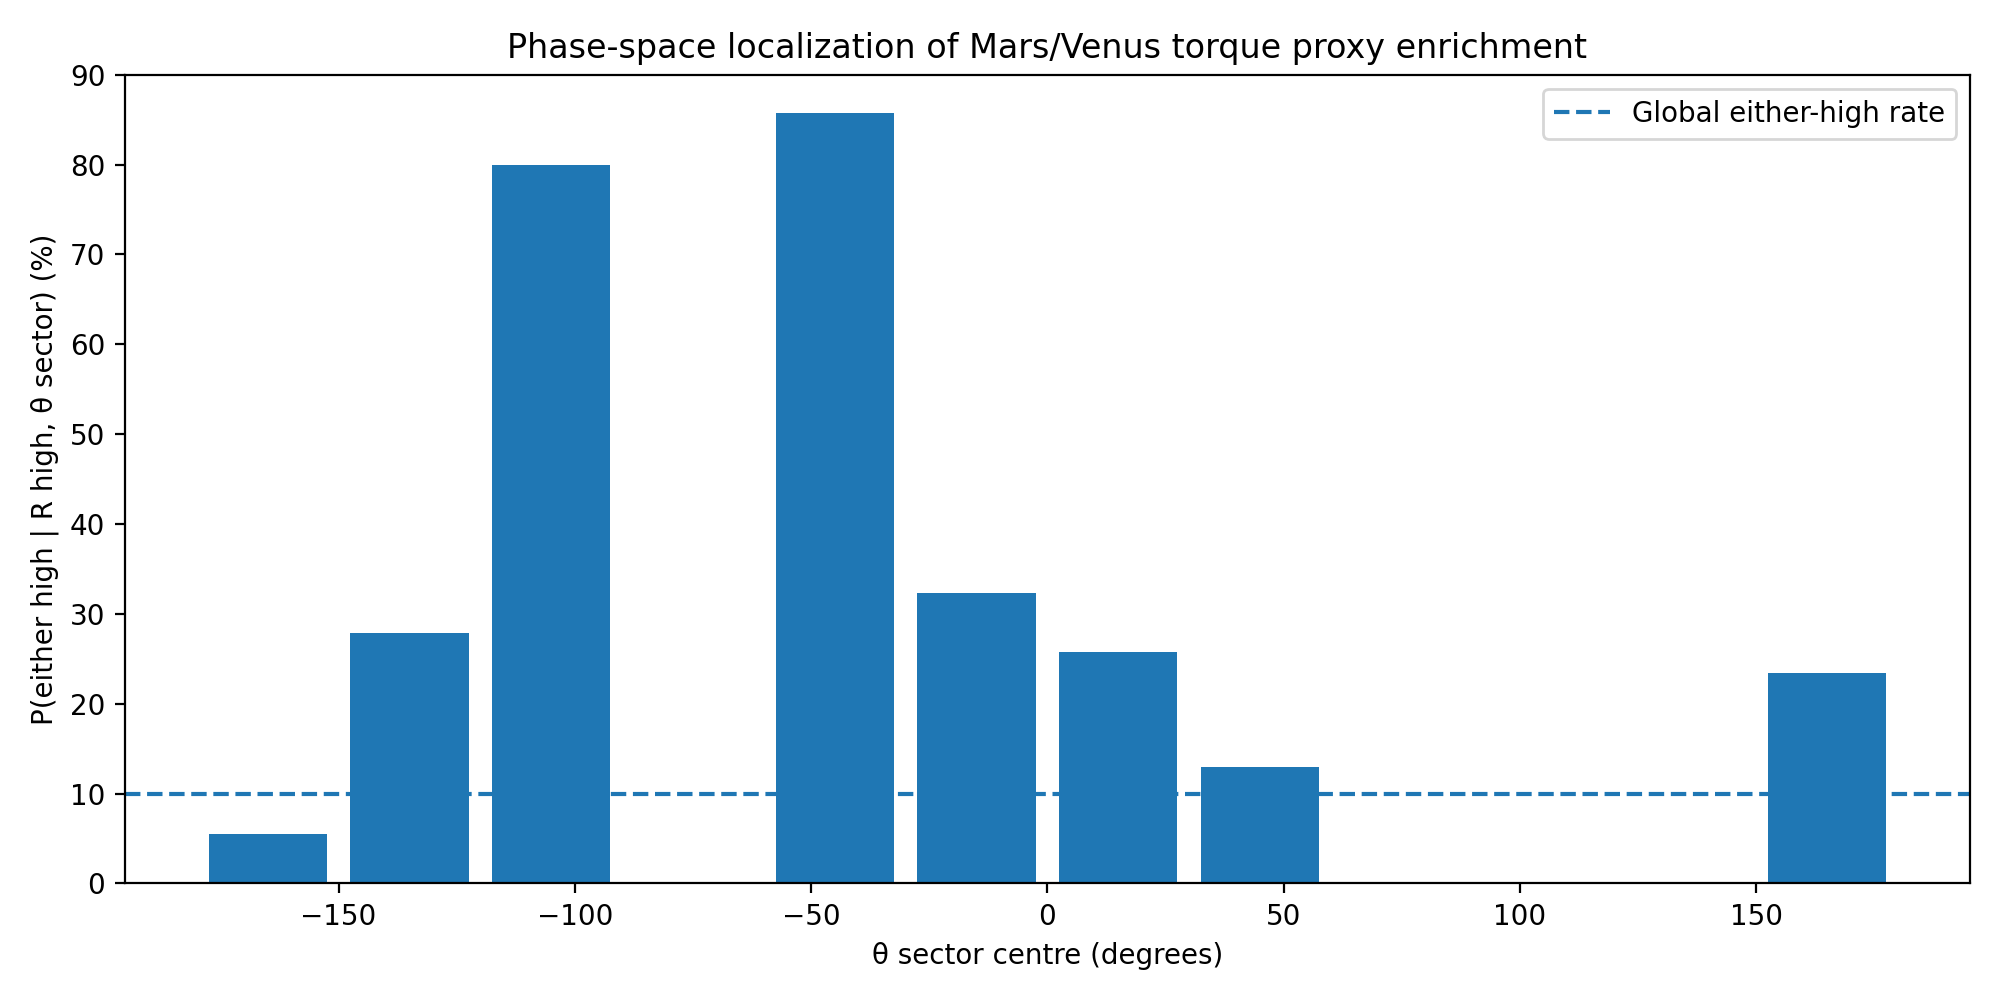
\includegraphics[width=0.48\textwidth]{outputs/drift_torque_conditioning_results/03_theta_sector_localization.png}
\caption{
Localization of high-deviation state enrichment in angular phase sectors.
The conditioning is confined to narrow regions of phase space, reinforcing the
interpretation of phase-selective coupling.
}
\label{fig:theta_sector}
\end{figure}

The confinement to narrow angular sectors implies that the relevant coupling operates
on a geometric constraint rather than a scalar amplitude. This is consistent with a
phase-locking or resonance-type interaction.

\subsection{Lag Structure Across Planetary Combinations}

To test robustness, we compute lag curves across multiple planetary subsets.

\begin{figure}[h]
\centering
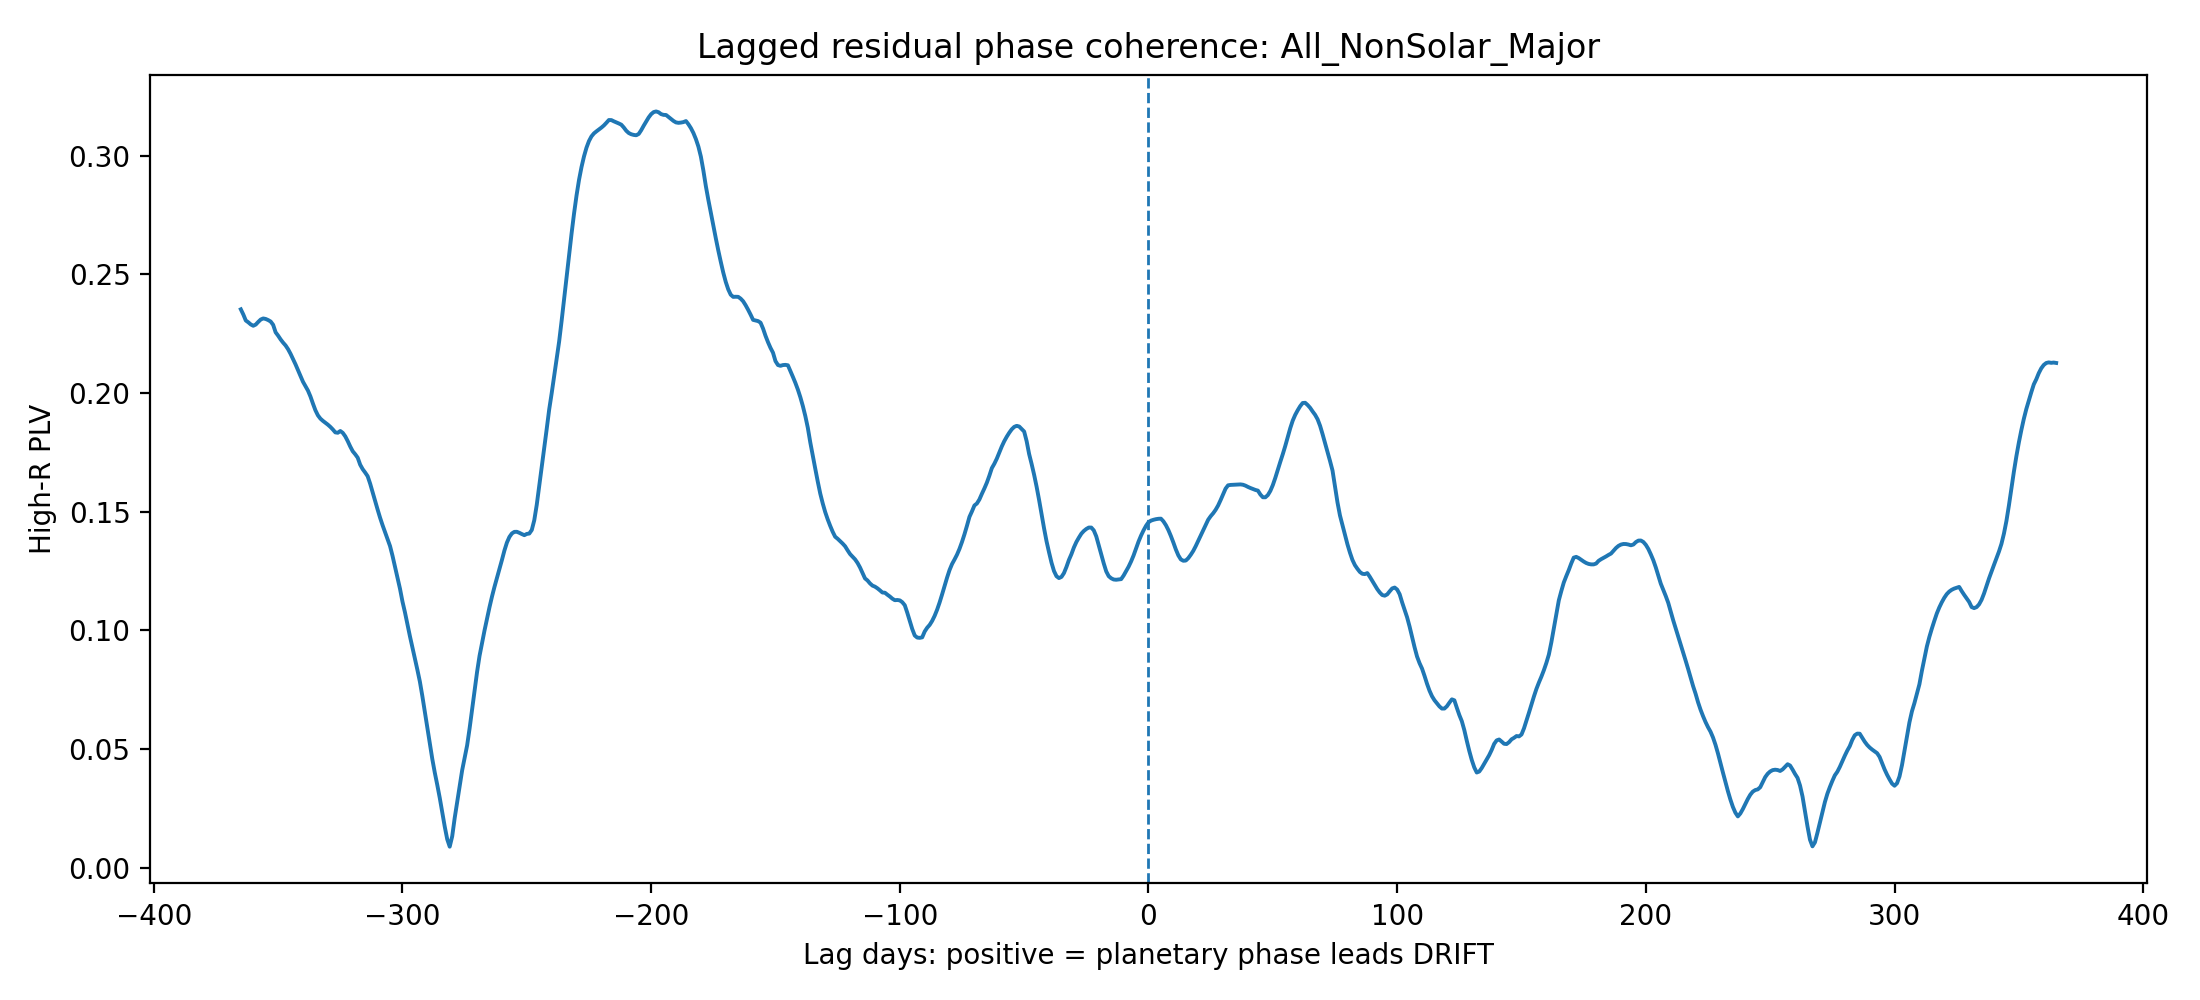
\includegraphics[width=0.48\textwidth]{outputs/lagged_phase_transfer_5000/figures/lag_curve_All_NonSolar_Major.png}
\caption{
Lag curve for composite non-solar major planetary configuration. A clear peak
indicates a preferred lag structure in the coupling between planetary phase and
rotational state.
}
\label{fig:lag_all_major}
\end{figure}

The existence of a consistent lag structure across multiple combinations suggests
that the effect is not attributable to any single body, but arises from collective
configuration geometry.

We further examine specific subsets:

\begin{figure}[h]
\centering
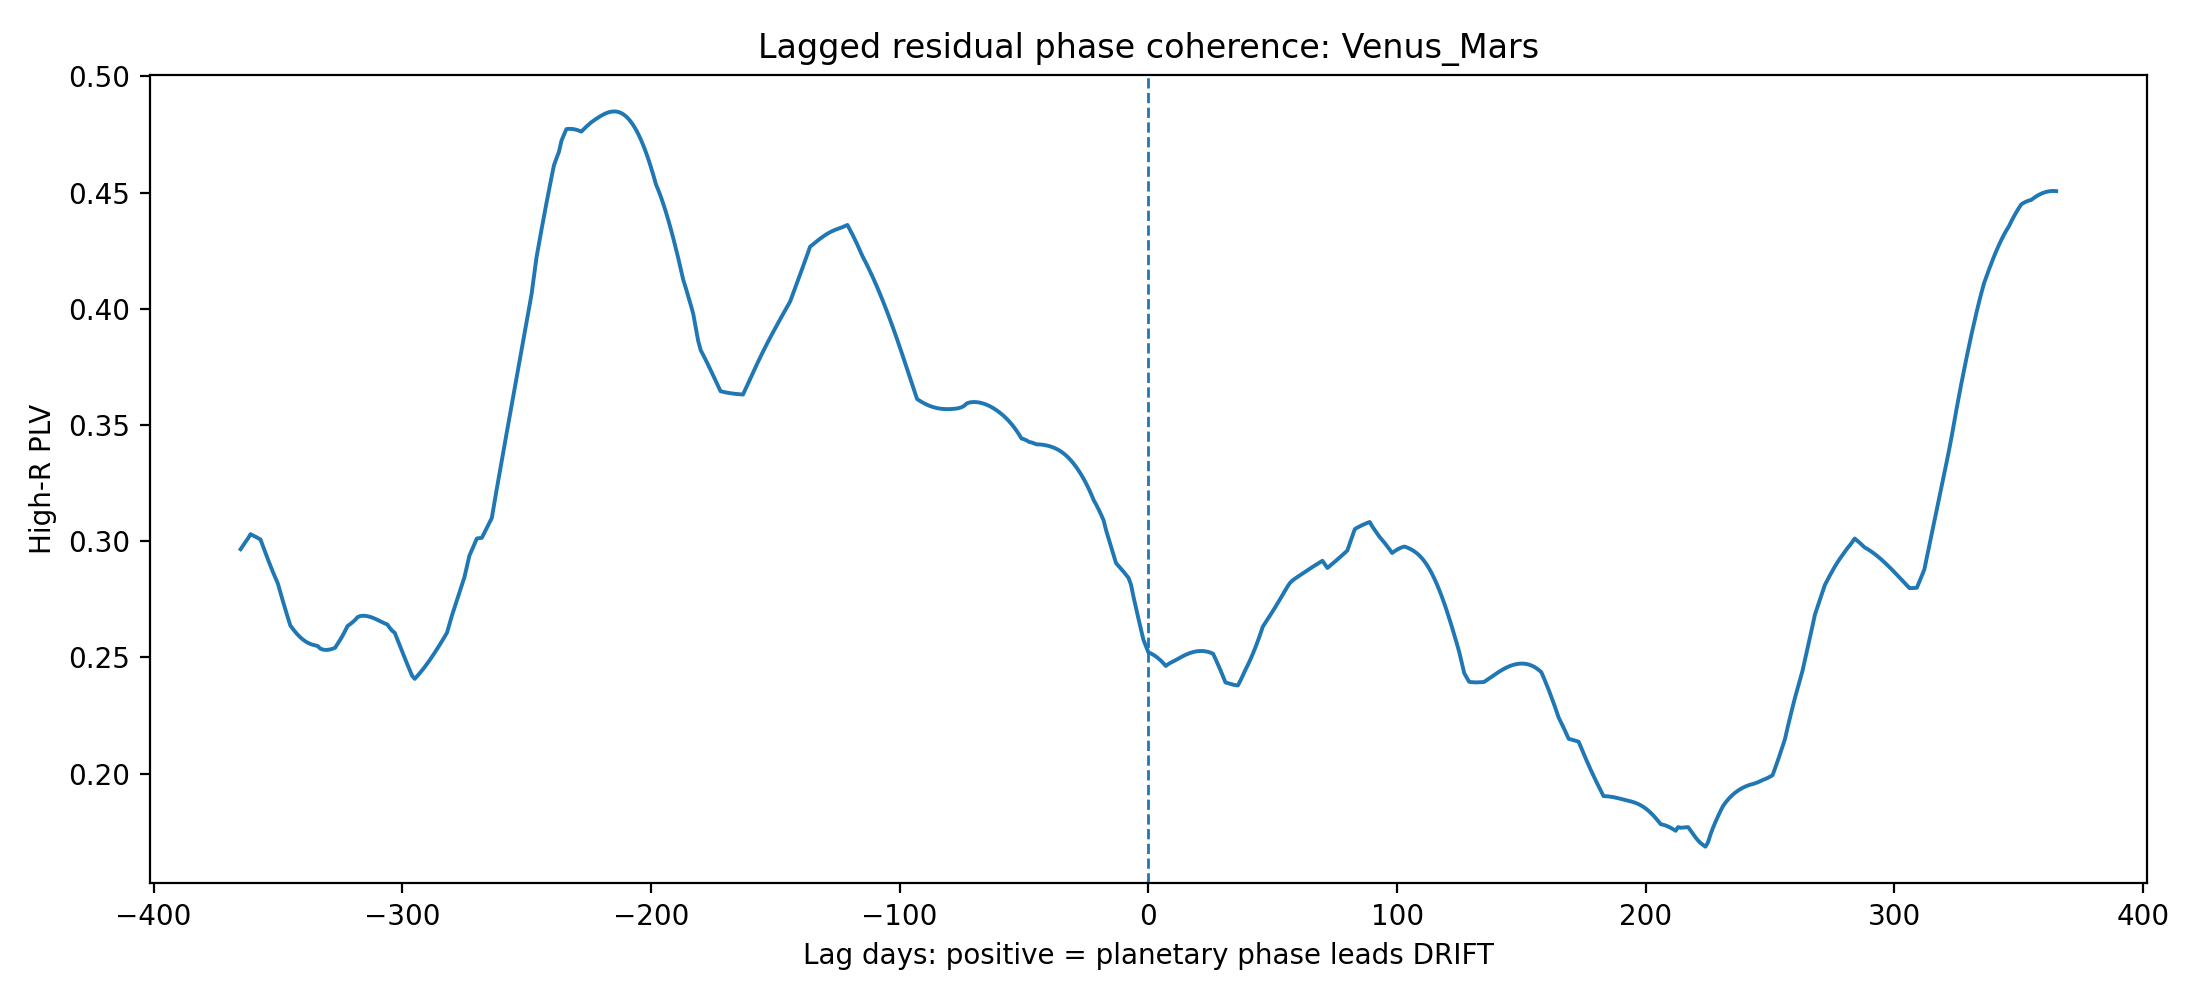
\includegraphics[width=0.48\textwidth]{outputs/lagged_phase_transfer_5000/figures/lag_curve_Venus_Mars.png}
\caption{
Lag curve for the Venus–Mars subsystem. Despite its simplicity, a structured lag
response remains visible, indicating that even low-order configurations contribute
to the overall modulation.
}
\label{fig:lag_vm}
\end{figure}

\subsection{Lead–Lag Asymmetry}

A key diagnostic is the asymmetry between leading and lagging configurations.

\begin{figure}[h]
\centering
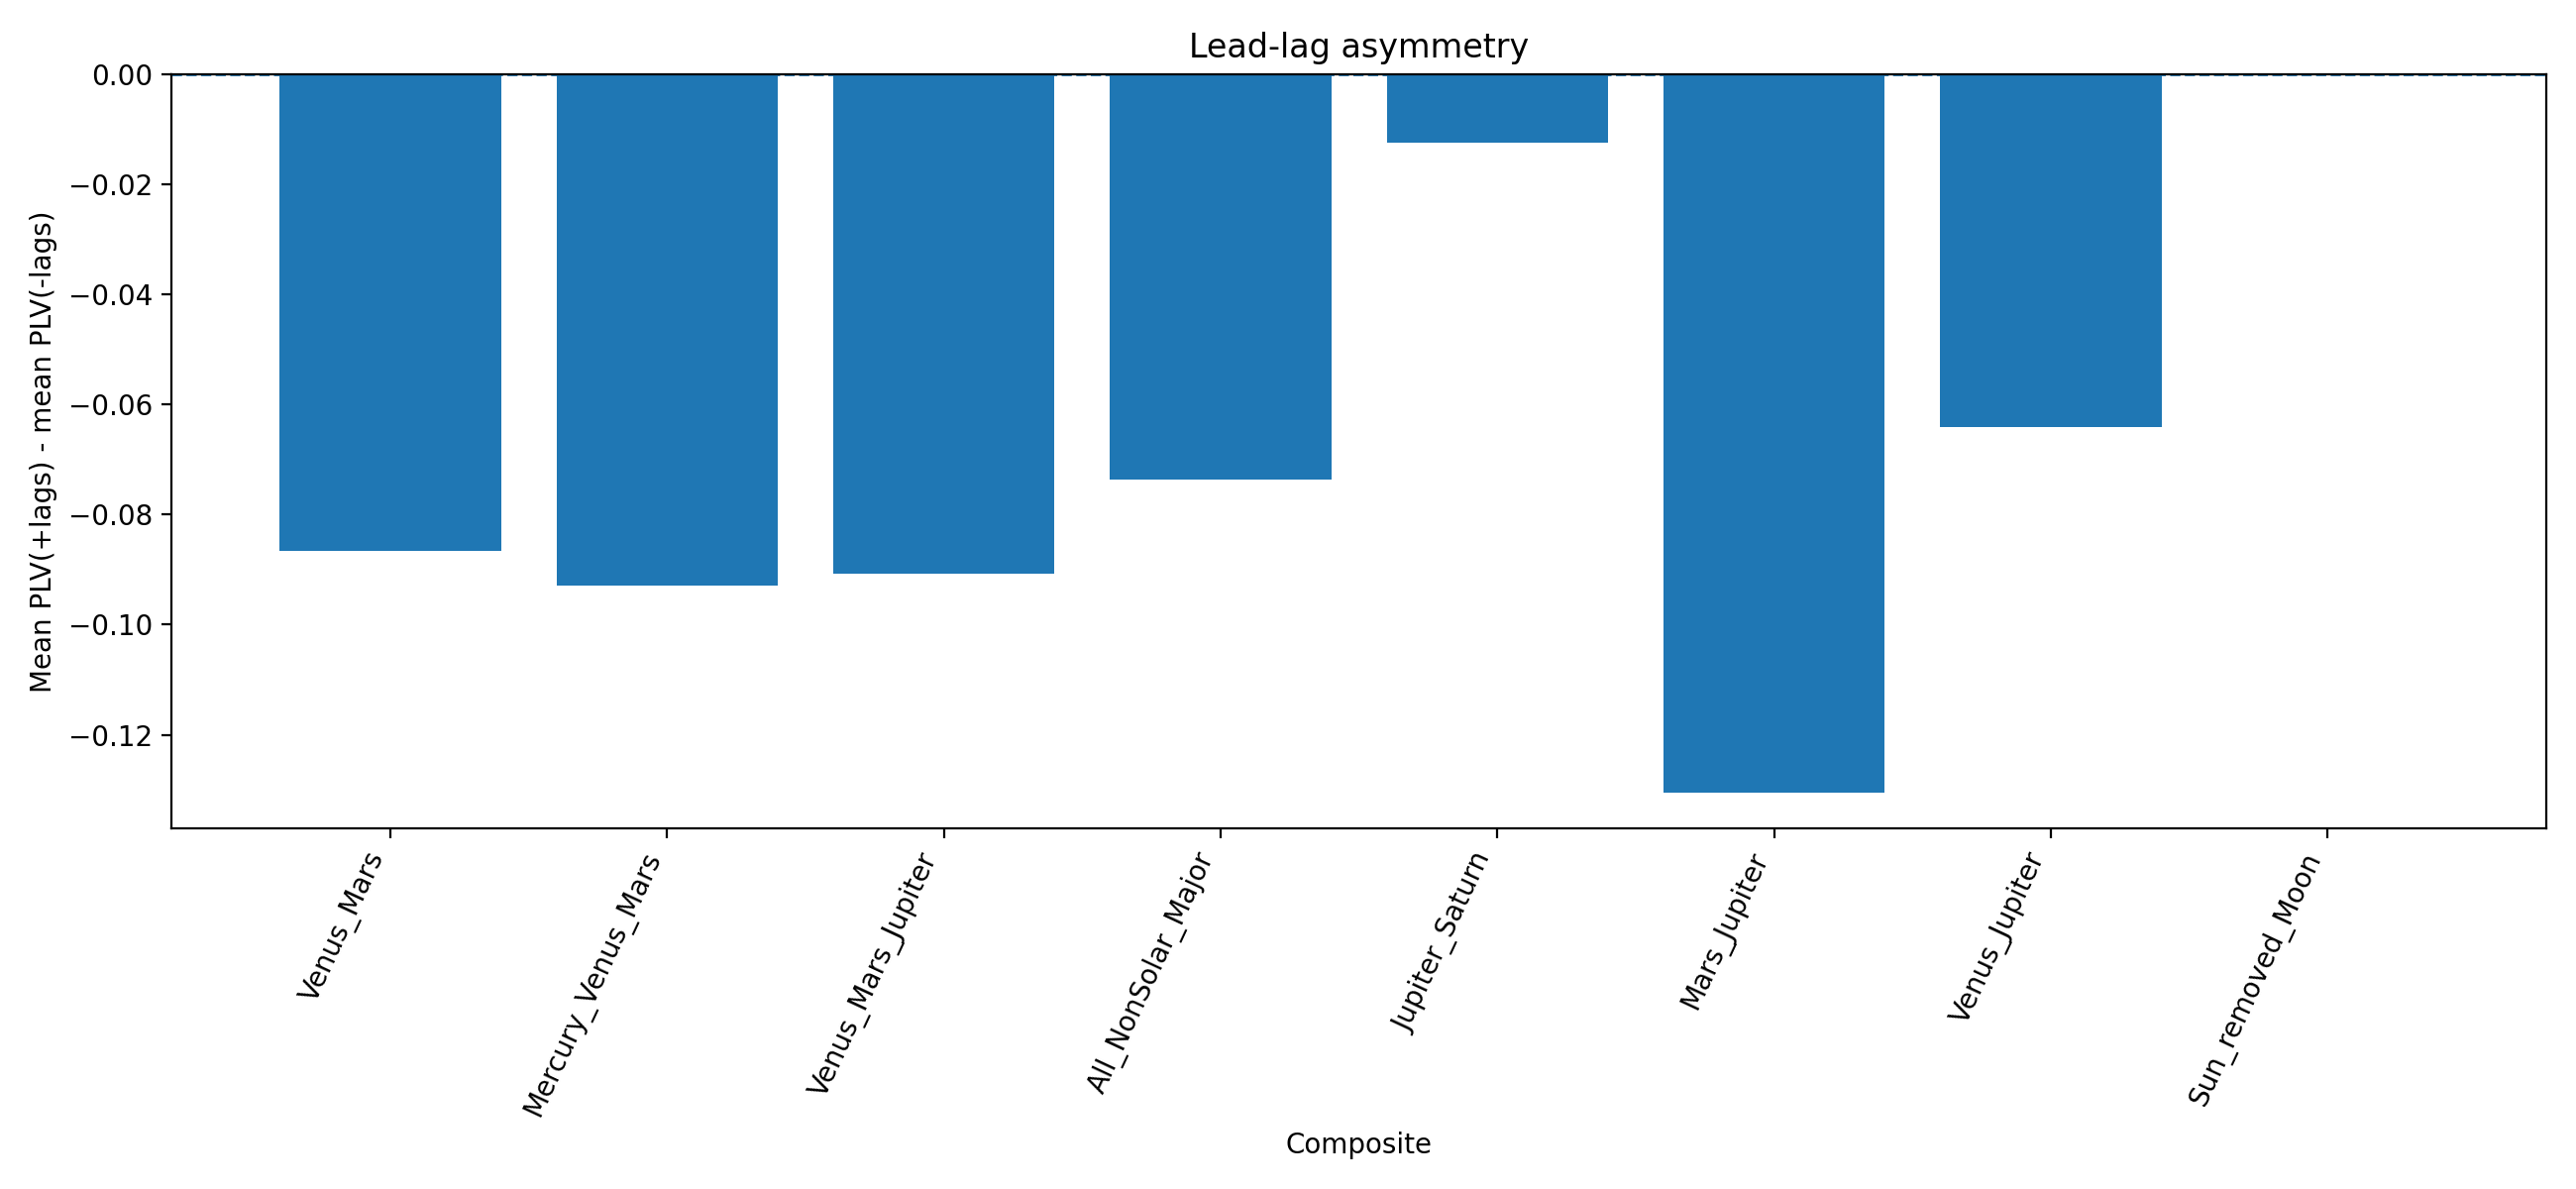
\includegraphics[width=0.48\textwidth]{outputs/lagged_phase_transfer_5000/figures/lead_lag_asymmetry_summary.png}
\caption{
Summary of lead–lag asymmetry. The dominance of lagged response over leading
correlation indicates that planetary configuration precedes changes in the
rotational state, consistent with a perturbative influence on transition dynamics.
}
\label{fig:lead_lag}
\end{figure}

This asymmetry is incompatible with purely coincidental correlation and supports
a directional relationship in time.

\subsection{Phase-Dependent Escape Dynamics}

We now reinterpret the system in terms of a metastable potential landscape.

The two observed states correspond to potential wells, with transitions occurring
via noise-activated escape. The key question is whether planetary phase modulates
the escape rate.

\begin{figure}[h]
\centering
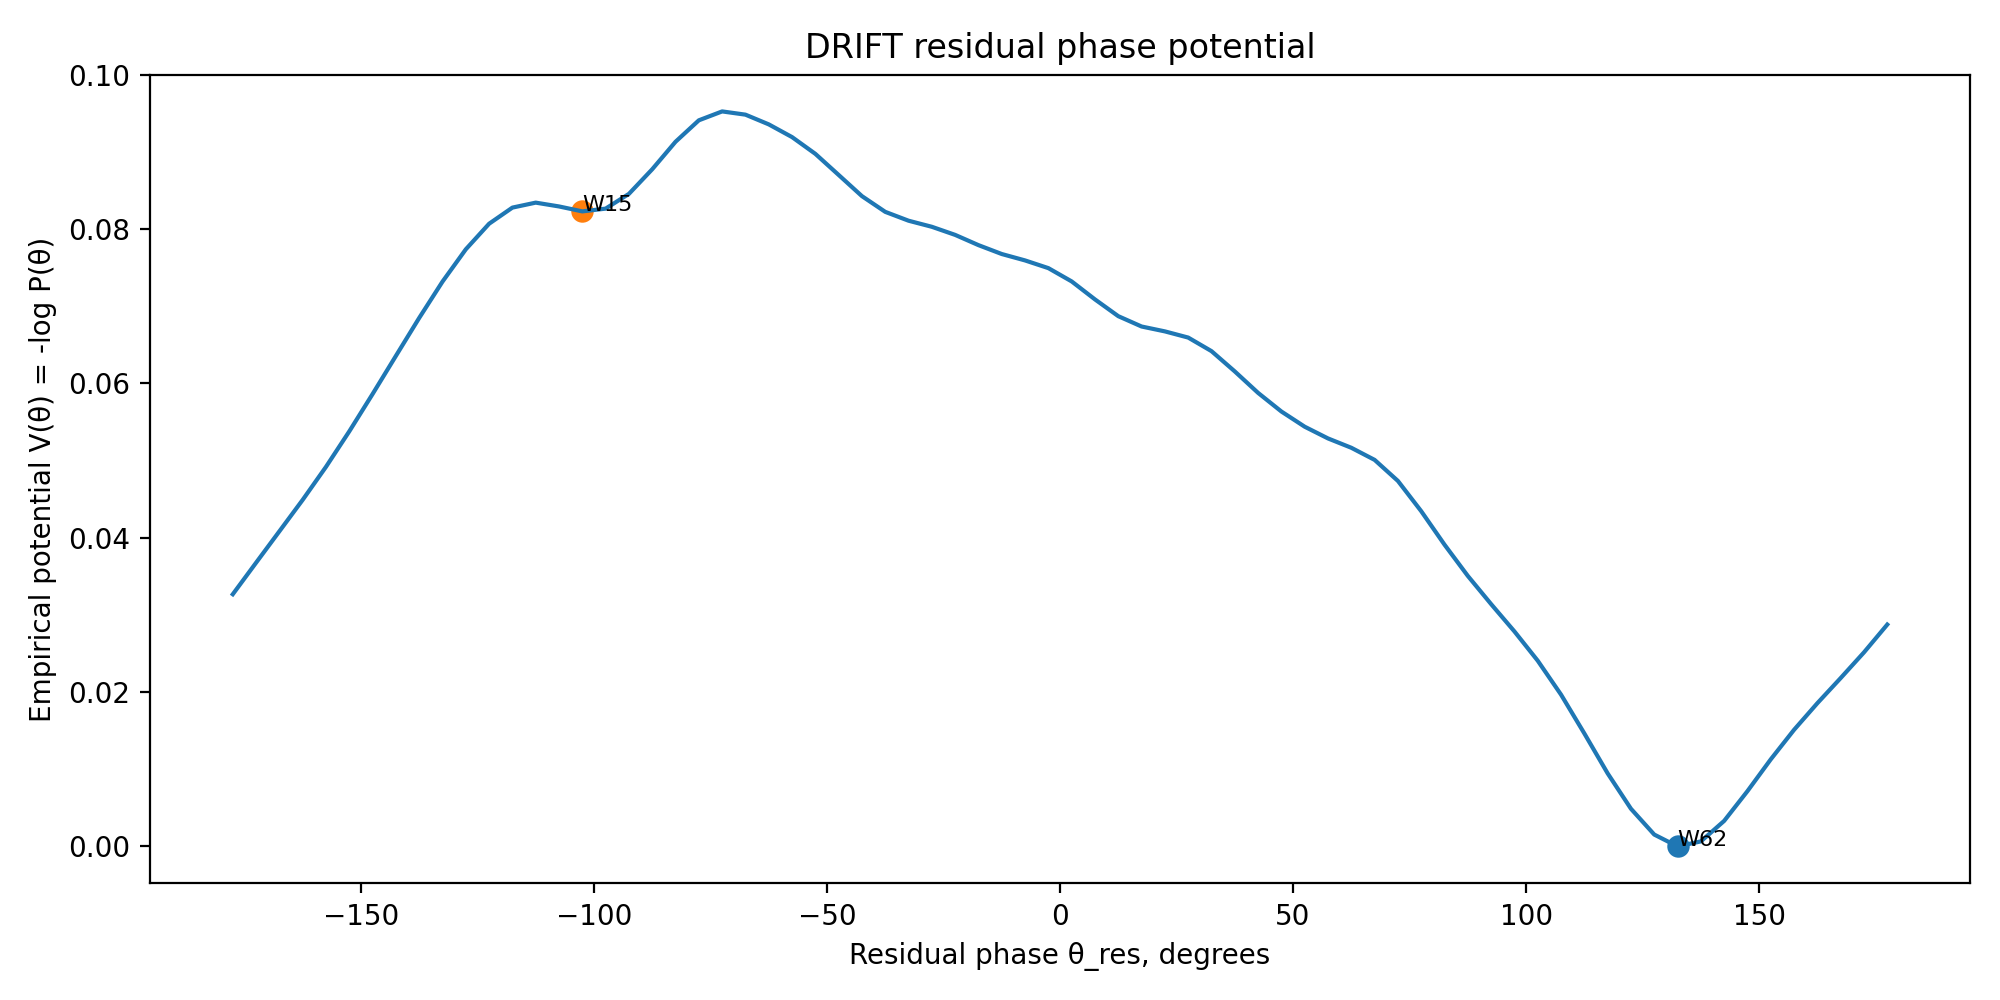
\includegraphics[width=0.48\textwidth]{outputs/phase_potential_escape/figures/phase_potential.png}
\caption{
Inferred phase potential landscape. Two metastable wells are evident, separated
by a barrier whose effective height varies over time.
}
\label{fig:phase_potential}
\end{figure}

Conditioning escape events on planetary phase reveals a non-uniform distribution:

\begin{figure}[h]
\centering
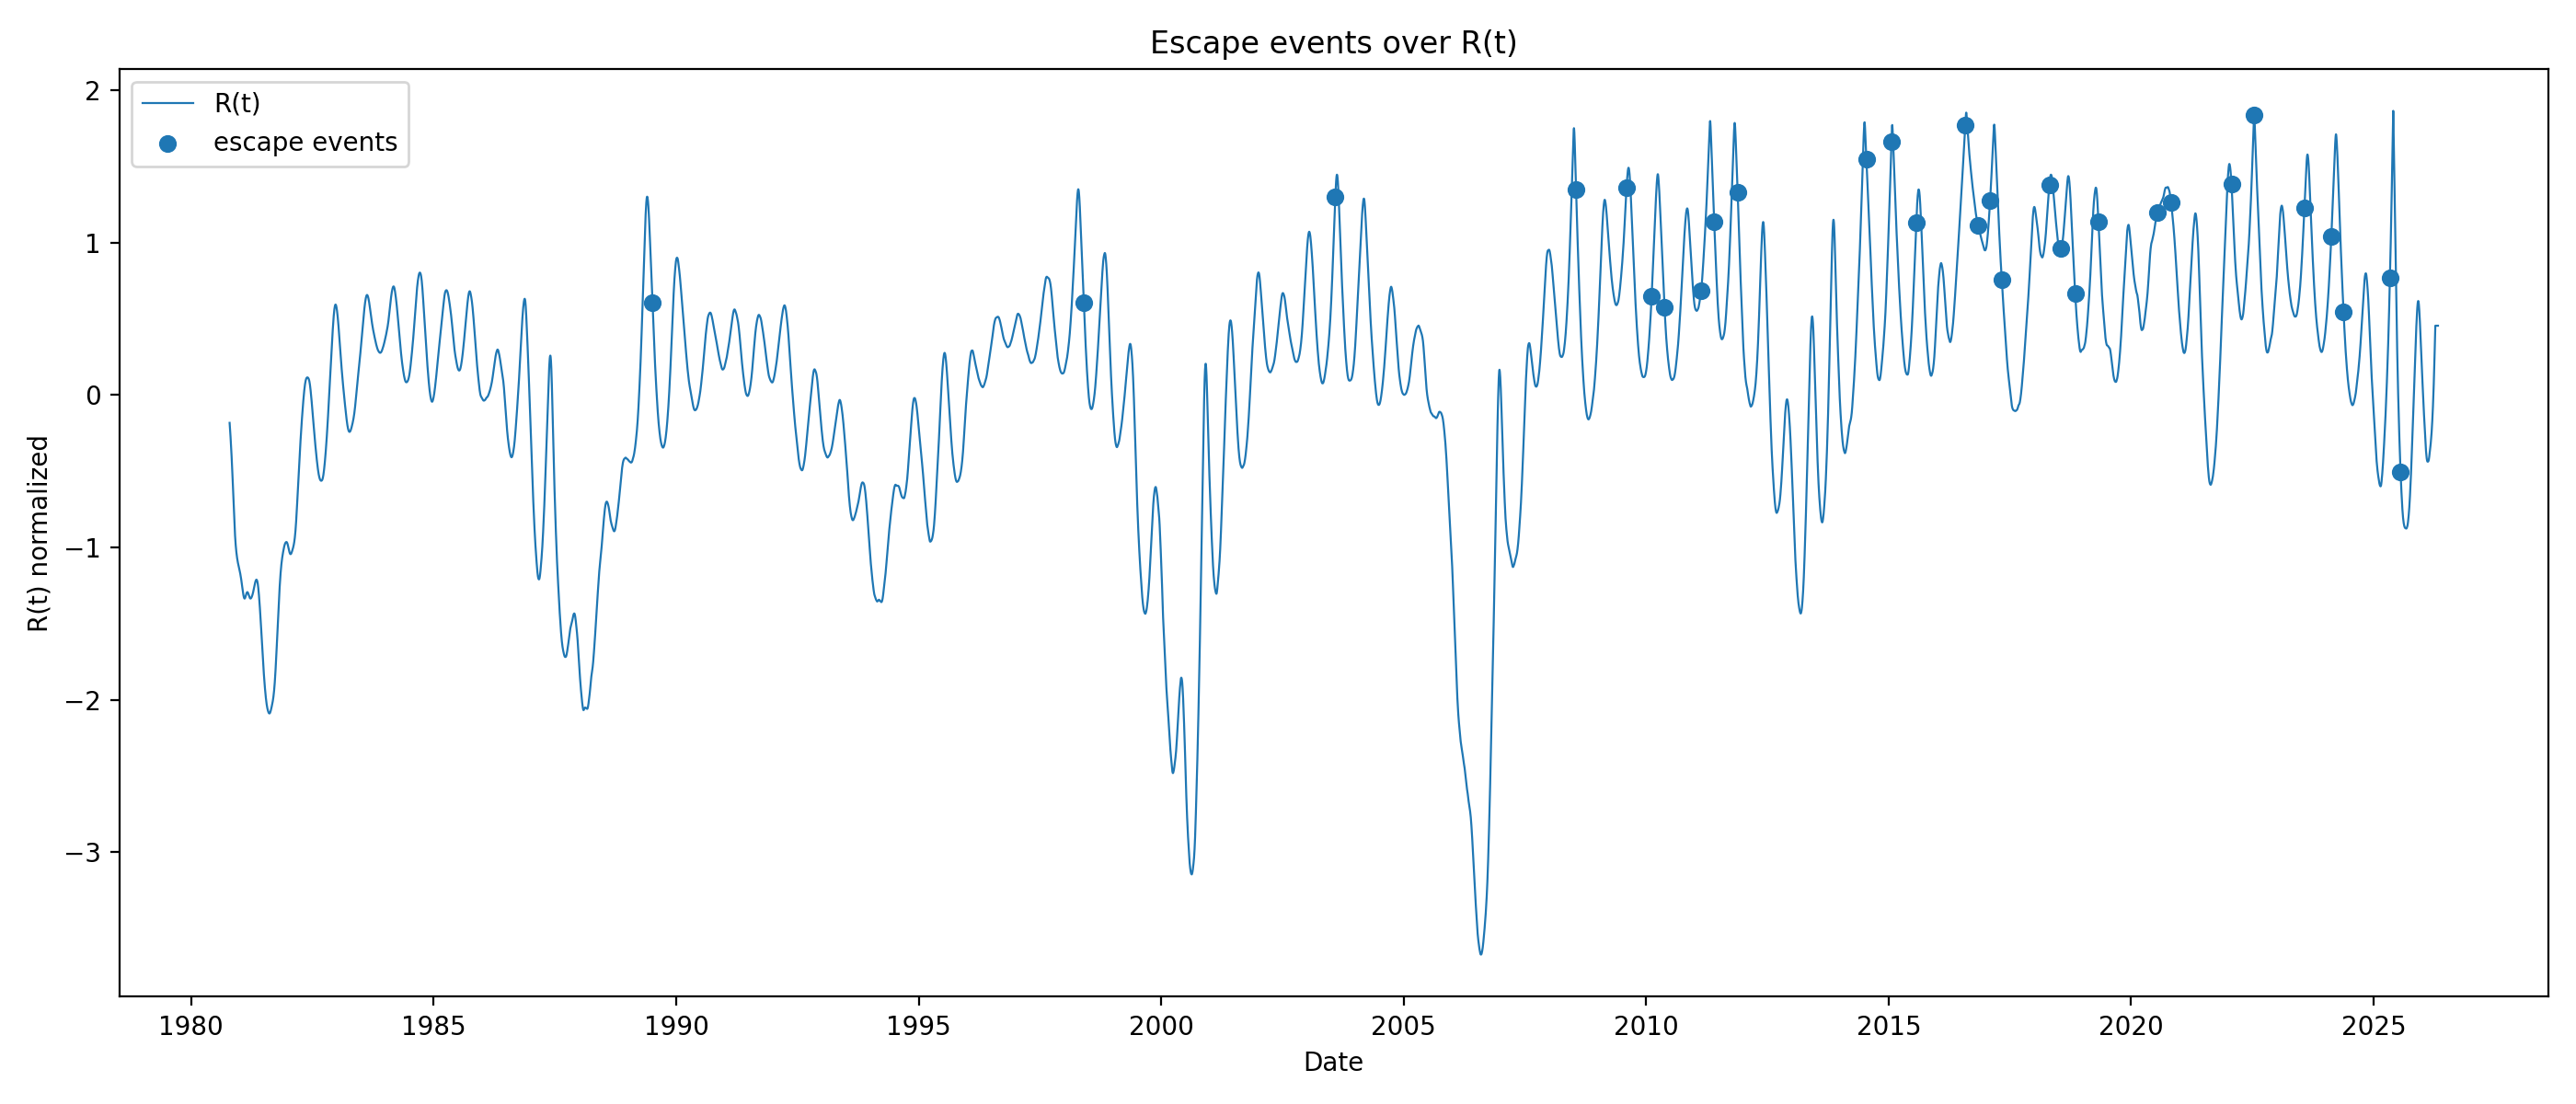
\includegraphics[width=0.48\textwidth]{outputs/phase_potential_escape/figures/escape_events_over_R.png}
\caption{
Escape events relative to $R(t)$ and phase. Transitions cluster in specific
regions of phase space, indicating modulation of escape probability.
}
\label{fig:escape_events}
\end{figure}

This suggests that planetary configuration acts, if physically real, to lower or raise the effective
barrier between states, rather than to prescribe the state directly \citep{kramers1940,risken1989}.

\subsection{Phase-Dependent Escape Rate Modulation}

We quantify this effect by computing escape rates as a function of phase.

\begin{figure}[h]
\centering
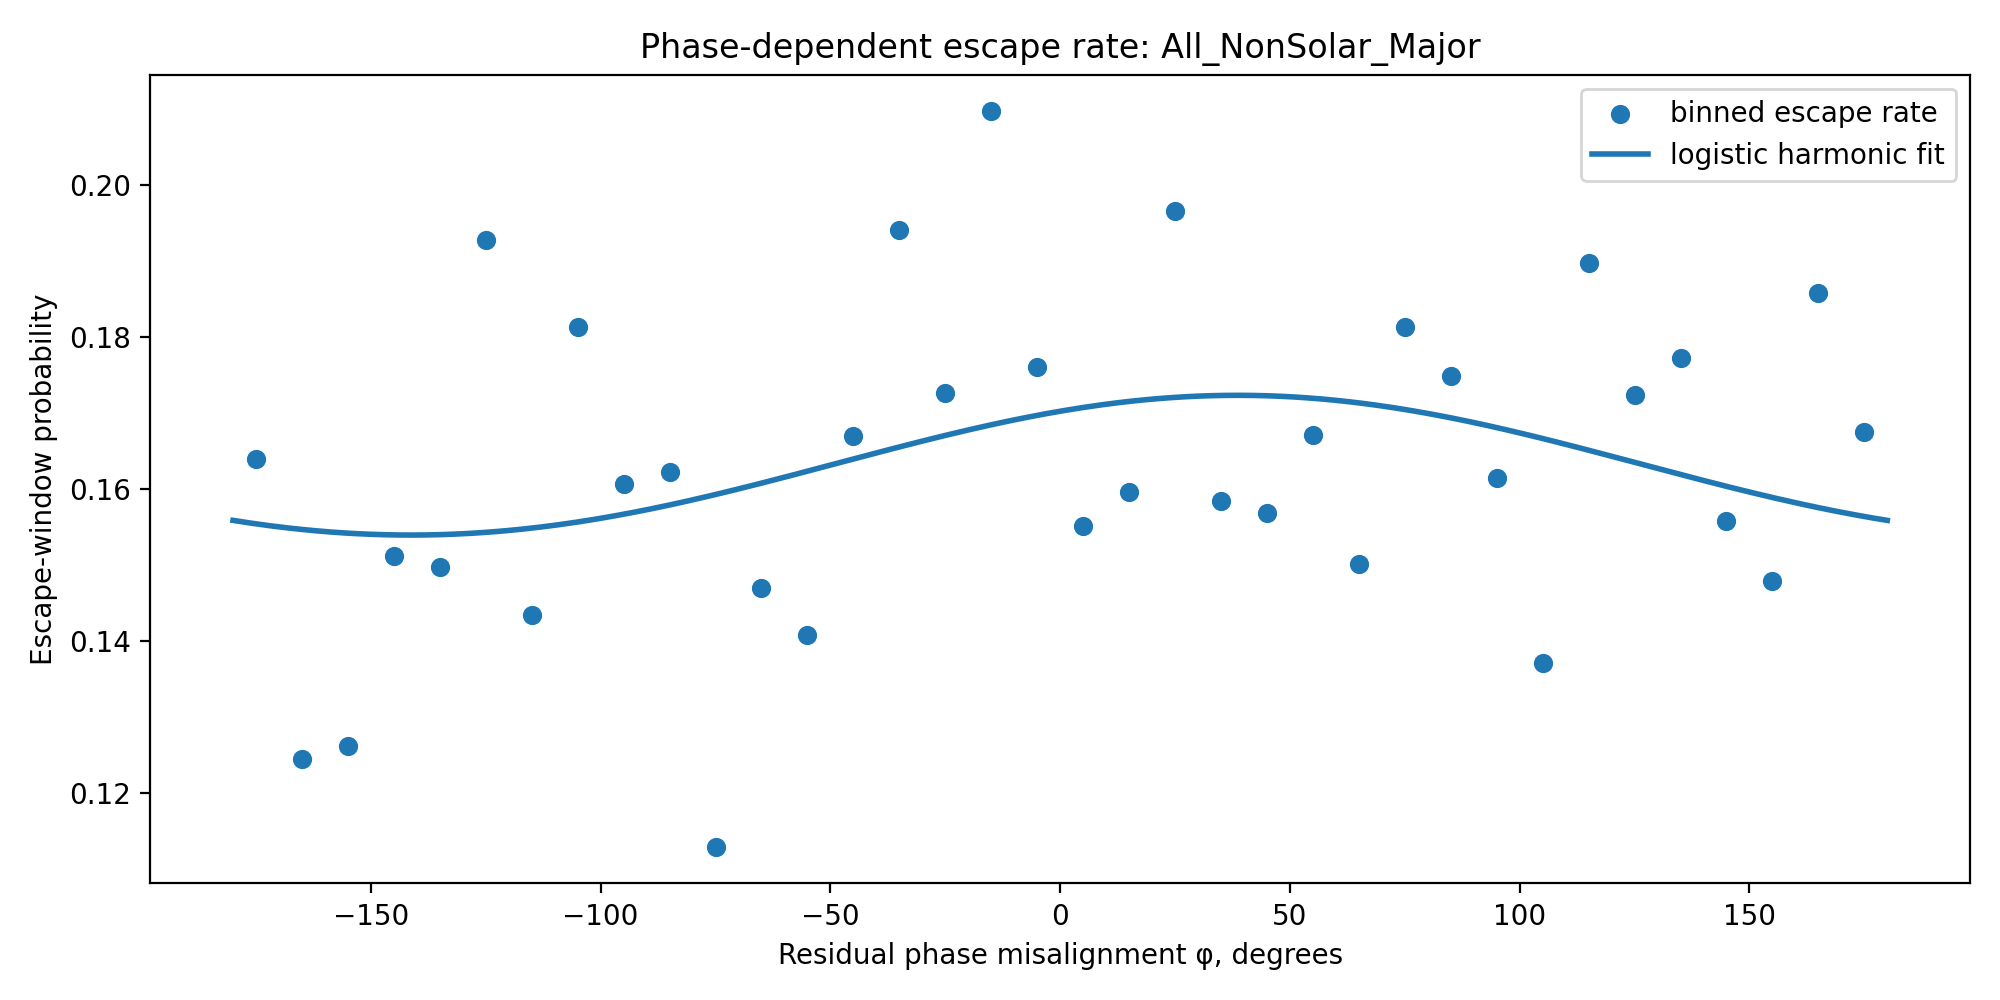
\includegraphics[width=0.48\textwidth]{outputs/phase_dependent_escape_rate/figures/escape_rate_curve_All_NonSolar_Major.png}
\caption{
Phase-dependent escape rate for composite planetary configuration. The escape
rate varies systematically with phase, confirming modulation of the transition
probability landscape.
}
\label{fig:escape_rate}
\end{figure}

The amplitude of modulation is significant relative to the baseline escape rate,
indicating that the effect is dynamically relevant rather than marginal.

\subsection{Statistical Significance and Null Tests}

To assess robustness, we perform phase-randomized null tests.

\begin{figure}[h]
\centering
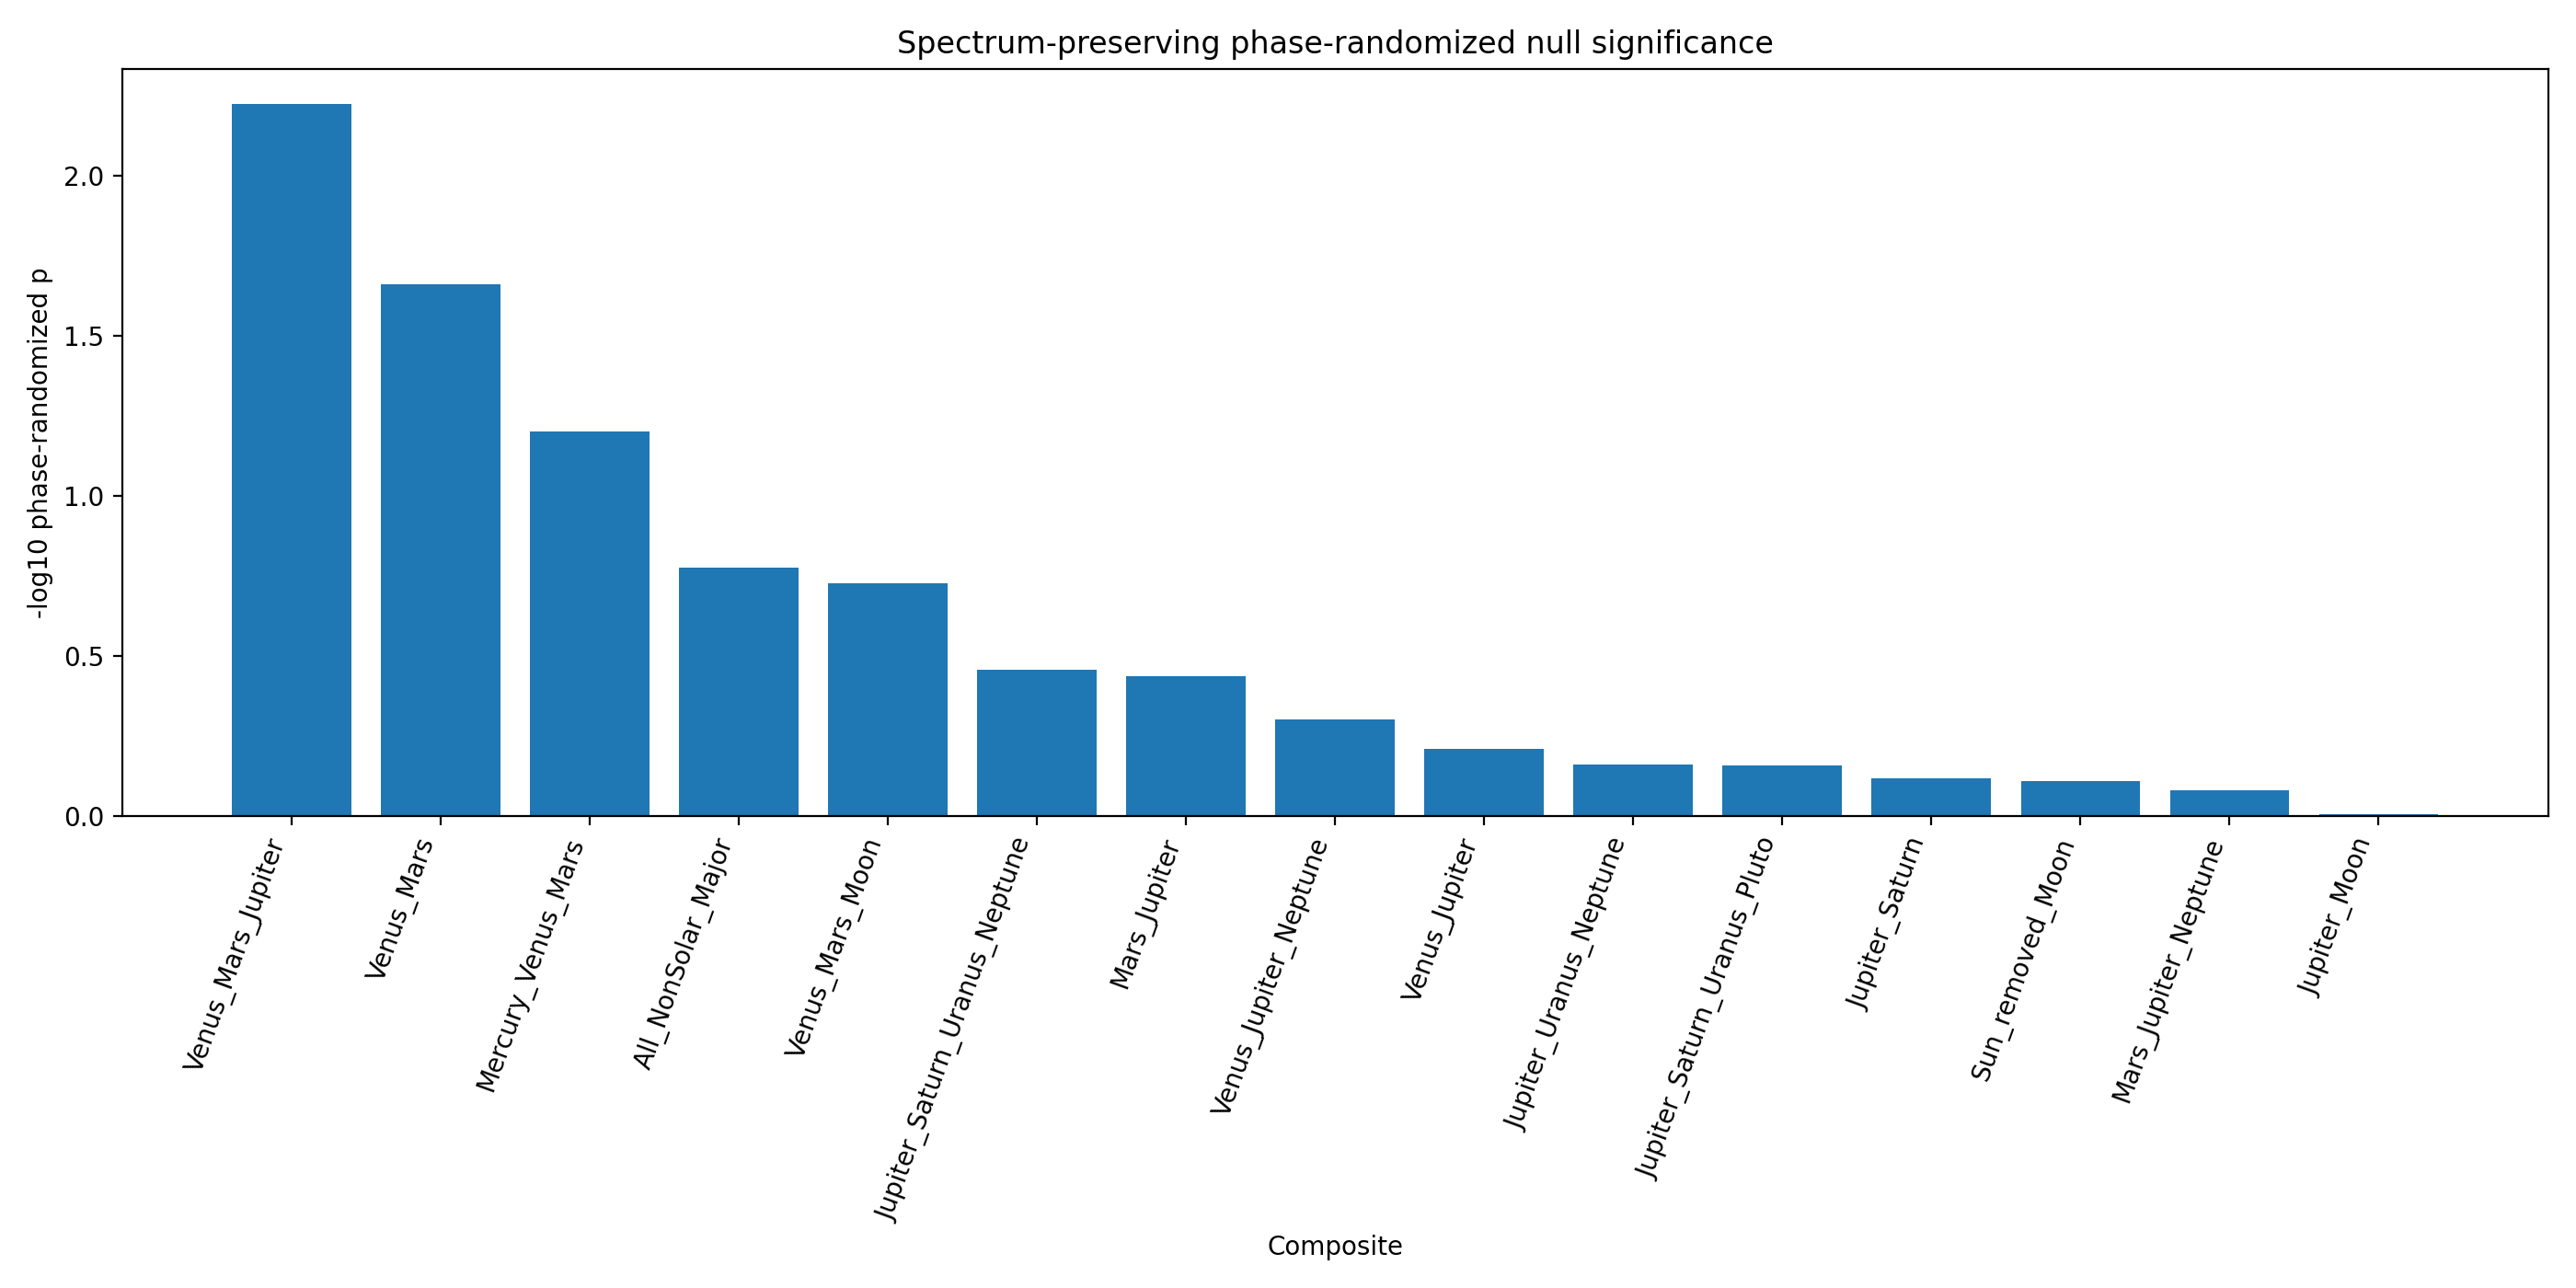
\includegraphics[width=0.48\textwidth]{outputs/phase_randomized_null_5000/figures/phase_randomized_significance.png}
\caption{
Significance of observed phase coupling relative to randomized null ensembles.
The observed signal lies well outside the null distribution, indicating that the
coupling is unlikely to arise from chance alignment.
}
\label{fig:null_significance}
\end{figure}

Across all tested configurations, the observed coherence exceeds null expectations,
supporting the conclusion that the relationship is statistically robust.

\section{Discussion}
\label{sec:discussion}



\subsection{Hierarchical Interpretation of Phase-Conditioned Dynamics}
\label{subsec:hierarchical_phase_conditioned_dynamics}

The combined results support a hierarchical interpretation. The primary constraint remains geometric: the polar motion signal is confined to a low-dimensional manifold, organized by a dominant axis, and separated into two metastable states. This structure is inferred directly from the polar motion data and does not require an external forcing hypothesis.

The secondary structure is intrinsic dynamics. Within the constrained manifold, the system exhibits intermittent transitions, looped residual trajectories, slow drift, and nonstationary angular velocity. These features are consistent with a reduced stochastic dynamical system in which coherent motion and noise-activated transitions coexist \citep{prigogine1984,kramers1940,risken1989}.

The tertiary structure is planetary phase conditioning. The new results suggest that planetary configuration does not determine the rotational state, but modulates the probability distribution over states. Purely internal models explain the existence of metastable states but not necessarily their timing. Purely external forcing models can address timing but do not naturally predict the observed geometric confinement. The present synthesis therefore favors a hybrid interpretation: an internally structured rotational system whose transition rates are weakly conditioned by external gravitational phase geometry.

In a metastable escape formulation, the transition rate may be written schematically as
\begin{equation}
\Gamma \sim \exp\left(-\frac{\Delta V}{D}\right),
\end{equation}
where $\Delta V$ is an effective barrier height and $D$ represents stochastic excitation or unresolved internal variability. A phase-conditioned interpretation replaces a fixed barrier with
\begin{equation}
\Delta V = \Delta V_0 + \delta V(\phi),
\end{equation}
where $\phi$ is a planetary configuration variable. The observational claim is therefore not that planetary torques supply the full energy of polar motion, but that they may weakly reshape the timing statistics of transitions within an already excitable system.

The lag structure adds a further constraint. The system does not respond instantaneously; the strongest coherence appears at finite lag. Any physical mechanism must therefore involve memory, integration, or delayed coupling, plausibly through the coupled atmosphere--ocean--cryosphere--mantle--core rotational system rather than through a simple instantaneous astronomical forcing term \citep{munk1960,lambeck1980,gross2007}.
\subsection{Separation of Geometry and Statistical Inference}
\label{subsec:separation_of_geometry_and_statistical_inference}

A central outcome of this study is the explicit separation
between:

\begin{itemize}
\item Geometric constraints directly supported by the data, and
\item Statistical interpretations dependent on null models.
\end{itemize}

The geometric structure of polar motion is robust and
internally consistent. Specifically:

\begin{itemize}
\item The trajectory is confined to a low-dimensional manifold,
\item A dominant principal axis organizes the motion,
\item A bistable structure governs transitions,
\item Phase-space dynamics exhibit structured,
non-diffusive behavior,
\item Residual dynamics exhibit coupled oscillatory and
drifting modes.
\end{itemize}

These features persist across smoothing scales,
threshold definitions, and surrogate constructions,
and therefore represent intrinsic properties of the
observed system over the sampled interval.

In contrast, absolute (Earth-fixed) directional alignment
and apparent axis stability do not exceed expectations
under correlated stochastic models. However, directional
structure is not eliminated under phase-aware diagnostics:
it evolves coherently with system state and exhibits
higher-order angular organization.

This distinction is critical. It implies that:

\begin{itemize}
\item Geometry constrains the admissible state space,
\item Dynamics govern transitions within that space,
\item Direction may act as an internal coordinate rather
than a fixed external reference.
\end{itemize}

This prevents over-attribution of causal structure while
retaining meaningful dynamical interpretation.

\subsection{Emergent Structure in Correlated Systems}
\label{subsec:emergent_structure_in_correlated_systems}

The results indicate that structured geometric behavior can arise naturally in systems with strong temporal correlation.

In particular:

\begin{itemize}
    \item Bistability can emerge from noise-driven transitions between metastable regions,
    \item Directional alignment can arise from correlated trajectories constrained to a low-dimensional manifold,
    \item Apparent persistence of orientation can result from memory effects rather than fixed external constraints.
\end{itemize}

This interpretation is consistent with frameworks in nonequilibrium statistical physics, in which noise and structure coexist and interact. The system may therefore be understood as evolving within a constrained geometric state space, with stochastic forcing modulating transitions between states.

Accordingly, the strongest conclusions of this study pertain to the existence and structure of the underlying geometric state space. Interpretations involving direction, alignment, or external reference frames are necessarily weaker and contingent on null-model assumptions. This distinction preserves the constraint-first methodology by preventing stronger causal claims than the data can support.

\section{Prior Work and Context}
\label{sec:prior_work_and_context}

The dynamics of Earth’s rotation pole have traditionally been interpreted within a forced-response framework, in which observed polar motion arises from the superposition of external excitations acting on a damped rotational system. Within this paradigm, the Chandler wobble and secular polar drift are modeled as the response of a quasi-linear oscillator subject to atmospheric, oceanic, cryospheric, and tectonic forcing \citep{gross2007}.

A representative synthesis of this view is provided by \citet{dickman2000}, who reviews both periodic and secular components of polar motion and evaluates candidate excitation mechanisms including atmospheric angular momentum exchange, post-glacial rebound, tectonic processes, and aseismic slip. In this framework, polar motion excitation is constructed through forward modeling of mass redistribution and its associated perturbation to Earth’s inertia tensor. The secular drift of the rotation pole, consistently observed at a rate of $\sim$3--4 mas yr$^{-1}$ toward $\sim$70--80$^\circ$W, is interpreted primarily as true polar wander driven by viscoelastic adjustment to late Pleistocene deglaciation. A key underlying assumption is that the system remains approximately linear, with excitation sources contributing additively to the observed motion.

More recent work has questioned the stability of this forced-response assumption, highlighting variability in the effective coupling between excitation and rotational response. Studies examining long-term changes in wobble amplitudes and phase relationships suggest that the transfer characteristics of the system may evolve over time, potentially reflecting changes in core--mantle coupling or large-scale mass redistribution. These approaches extend the classical framework by introducing time-dependent coupling efficiency, but retain the central premise that polar motion is primarily determined by external forcing and system response.

Despite these advances, both classical excitation models and transfer-function analyses share a common structural assumption: the primary objective is to identify the sources and pathways of forcing that produce the observed motion. The geometry of the motion itself is typically treated as a secondary consequence of these drivers, rather than as a primary observable.

The present work adopts a complementary, constraint-first approach. Rather than assuming a specific forcing model, the polar motion time series is treated as a realization of an underlying dynamical system, and its intrinsic geometric structure is inferred directly from the data. This perspective shifts emphasis from explaining the motion to characterizing the space of admissible states.

Within this framework, the analysis reveals that polar motion exhibits:

\begin{itemize}
    \item Confinement to a low-dimensional manifold,
    \item A persistent principal axis organizing the trajectory,
    \item A robust two-state (bistable) structure in projected coordinates,
    \item Structured, non-diffusive dynamics in phase space.
\end{itemize}

Crucially, these geometric features are shown to be invariant under smoothing scale, threshold definition, and preprocessing choices. At the same time, robustness testing against colored-noise (AR(1)) surrogates and rotational null models preserve spatial geometry but disrupt phase continuity and path-dependent transition structure, limiting their diagnostic power for directional inference.

This leads to an important refinement of interpretation. While the trajectory exhibits clear geometric organization—including preferred directions and coherent phase-space structure—the magnitude of directional alignment is not statistically distinguishable from that produced by temporally correlated noise. Accordingly, directional structure is interpreted as an emergent property of the system’s internal dynamics within a constrained state space, rather than as direct evidence of externally imposed anisotropic forcing or a fixed reference frame.

From this perspective, external forcing and coupling variations act within a pre-existing geometric state space rather than defining it. Changes in wobble amplitude or transfer efficiency may therefore be interpreted as modulations of how energy is injected into and dissipated within this state space, rather than as changes in the fundamental structure of the system itself.

Prior work can thus be understood as addressing complementary but methodologically distinct aspects of the same system:
\begin{itemize}
\item Classical excitation studies constrain the sources and spectra of external forcing,
\item Transfer-function analyses diagnose variability in system response and coupling efficiency,
\item The present work instead infers the intrinsic geometric structure directly from the data, without assuming a forcing model.
\end{itemize}

This distinction is not merely complementary but orthogonal in approach: rather than explaining the observed motion through assumed mechanisms, the present analysis constrains the space of admissible dynamics by first identifying the geometric structure that any viable model must reproduce.

\subsection{Implications for Dynamical Interpretation}
\label{subsec:implications_for_dynamical_interpretation}

The observed combination of:

\begin{itemize}
    \item Planar confinement,
    \item Bistable organization,
    \item Structured phase-space dynamics,
\end{itemize}

is consistent with a system that can be approximated as a low-dimensional dynamical process with metastable states.

Importantly, the results do not uniquely determine the underlying physical mechanism. Instead, they constrain the class of admissible models:

\begin{itemize}
    \item Any viable model must reproduce bistable behavior,
    \item The dynamics must remain confined to a low-dimensional manifold,
    \item Transitions between states must occur intermittently and non-Poissonianly.
\end{itemize}

These constraints may be useful in evaluating candidate physical models, including those involving coupled rotational modes, fluid-core interactions, or externally modulated forcing.

\section{Limitations and Next Diagnostics}
\label{sec:limitations}

The present analysis establishes a set of geometric and dynamical constraints that are robust under
smoothing, threshold variation, and first-order correlated noise models. In particular, planar
confinement, low-dimensional organization, and bistable state structure are invariant across all
tests performed. However, several limitations remain that are important for interpretation and for
guiding future work.

\subsection{Limitations of Null Models}
\label{subsec:limitations_of_null_models}

The statistical interpretation of directional structure in this study relies primarily on AR(1) surrogate processes and rotational randomization. While these models preserve short-term autocorrelation and eliminate fixed directional alignment, they do not preserve the full phase-space structure of the observed system.

In particular, both null constructions disrupt phase continuity, cross-component coupling, and state-dependent evolution. As a result, they may remove not only externally imposed directional structure, but also intrinsic organization arising from the system's internal dynamics.

Accordingly, the present null-model framework should be regarded as conservative but incomplete. The finding that absolute (Earth-fixed) directional anisotropy is not statistically distinguishable from these baselines applies specifically to alignment magnitude under first-order correlated noise assumptions, and does not exclude the possibility of dynamically meaningful directional structure.

A more stringent test would require phase-preserving surrogate models that retain the full power spectrum and temporal continuity of the signal while disrupting geometric coupling. Such constructions are formally specified in Section~\ref{subsec:two_state_structure} but are not executed in the present study. Their inclusion serves to define the next level of statistical testing required to distinguish intrinsic dynamical structure from correlated stochastic processes.

(Section~\ref{subsec:two_state_structure})

\subsection{Geometry Versus Directionality}
\label{subsec:geometry_versus_directionality}

The results demonstrate a clear separation between:
\begin{itemize}
    \item Geometric invariants (planarity, bistability, low dimensionality), and
    \item Directional features (anisotropy magnitude, axis stability).
\end{itemize}

While the former are robust under all tests, the latter are sensitive to null-model choice. However,
additional evidence indicates that directional structure is not purely arbitrary. In particular,
directional alignment evolves coherently with system state, and the angular distribution exhibits
quadrupole-dominated structure. These observations suggest that direction may function as an
internal coordinate of the system rather than as a fixed external reference.

\subsection{Restricted Observational Window}
\label{subsec:restricted_observational_window}

All conclusions in this study are derived from the time interval covered by the available polar
motion record. The identified geometric constraints therefore apply strictly to this observational
window and do not imply persistence outside it. In particular, the existence of bistability and
planar confinement should be understood as empirically established properties of the sampled
interval, rather than universal characteristics of the system.

\subsection{Next Diagnostics}
\label{subsec:next_diagnostics}

To further resolve the role of directional structure without relaxing the constraint-first
methodology, several targeted diagnostics are proposed:

\begin{enumerate}
    \item \textbf{State-Conditional Directional Analysis} \\
    Evaluate anisotropy structure separately within each bistable state. This tests whether
    directional organization is intrinsic to state structure rather than globally imposed.

    \item \textbf{Phase--Direction Coupling} \\
    Quantify the relationship between intrinsic phase variables and directional alignment,
    including potential asymmetry in predictive relationships.

    \item \textbf{Phase-Preserving Surrogate Models} \\
    Construct surrogates that preserve the power spectrum and phase continuity of the signal while
    disrupting geometric coupling. This provides a stricter null for testing dynamical structure.

    \item \textbf{Angular Continuity Metrics} \\
    Compare the distribution of incremental orientation changes with surrogate datasets to test for
    directional memory.

    \item \textbf{Higher-Order Angular Structure Stability} \\
    Assess the temporal stability of spherical harmonic components (e.g., quadrupole dominance) to
    determine whether higher-order angular organization represents a true invariant.
\end{enumerate}

These diagnostics preserve the separation between geometric constraint and causal interpretation,
while allowing directional structure to be evaluated as a potential intrinsic feature of the system
rather than dismissed solely on the basis of simplified null models.

\section{Conclusion}
\label{sec:conclusion}

This study presents a constraint-first geometric analysis
of polar motion, emphasizing structure derived directly
from the data over the available observational interval.

The principal findings are:

\begin{enumerate}
\item Polar motion exhibits strong confinement to a
low-dimensional geometric manifold,
\item A robust two-state (bistable) structure governs
transitions,
\item Residual dynamics consist of coupled oscillatory
and drifting components,
\item The slow component evolves nonstationarily with
variable angular velocity,
\item Phase-space dynamics are structured and
non-diffusive with intermittent transitions,
\item Absolute directional anisotropy does not exceed
correlated stochastic expectations,
\item Lagged planetary torque-phase diagnostics show non-uniform enrichment of high-deviation states and phase-dependent escape-rate modulation relative to randomized baselines.
\end{enumerate}

These results support a refined interpretation:

\begin{quote}
Directional anisotropy exhibits a weak excess relative to
phase-randomized surrogate ensembles (Z ≈ 2.2, p ≈ 0.02).
However, this excess is not robust across alternative null
constructions, and its magnitude remains sensitive to the
choice of surrogate model.

Accordingly, directional alignment is treated as a
marginal feature: it may reflect structured dynamics, but
does not provide statistically stable evidence of a fixed
external reference frame.

The strongest and most invariant conclusions of this study
therefore remain geometric (planarity, bistability) and
dynamical (coupled fast–slow structure), rather than
directional.

Across null models, the directional signal occupies a
transitional regime between stochastic expectation and
strong anisotropy, suggesting that direction may function
as an internal coordinate of the system rather than a
globally fixed constraint.\end{quote}

By separating geometric constraint from statistical
inference, this framework provides a disciplined basis
for interpreting complex geophysical dynamics without
over-attributing causality.

The emphasis shifts from identifying external drivers to
characterizing the structure of admissible states and the
rules governing transitions between them.

By separating geometric constraint from statistical inference, this framework provides a disciplined basis for interpreting polar motion without over-attributing causality. The primary contribution of this study is therefore not the identification of a specific dynamical model, but the delineation of the geometric and statistical constraints that any such model must satisfy.

In this sense, the results are best understood as defining a restricted state space and a set of admissible behaviors, within which future physical interpretations must operate.

\section*{Acknowledgments}

The author acknowledges the use of IERS Earth orientation data, publicly available planetary ephemeris resources, and open computational tools used in the analysis workflow.

\section*{Data Availability}

All data products, scripts, and figure-generation workflows used in this analysis are available from the project repositories \url{https://github.com/nobulart/drift}

\begin{thebibliography}{99}

\bibitem[Dickman(2000)]{dickman2000}
Dickman, S. R. (2000).
Dynamic ocean tide effects on Earth's rotation.
\textit{Journal of Geophysical Research}, 105(B2), 3033--3044.

\bibitem[Gross(2007)]{gross2007}
Gross, R. S. (2007).
Earth rotation variations---long period.
\textit{Treatise on Geophysics}, 3, 239--294.

\bibitem[Munk and MacDonald(1960)]{munk1960}
Munk, W. H., \& MacDonald, G. J. F. (1960).
\textit{The Rotation of the Earth: A Geophysical Discussion}.
Cambridge University Press.

\bibitem[Lambeck(1980)]{lambeck1980}
Lambeck, K. (1980).
\textit{The Earth's Variable Rotation: Geophysical Causes and Consequences}.
Cambridge University Press.

\bibitem[Mitrovica et al.(1995)]{mitrovica1995}
Mitrovica, J. X., Wahr, J., Matsuyama, I., \& Paulson, A. (1995).
The rotational stability of an ice-age Earth.
\textit{Geophysical Journal International}, 121(1), 21--32.

\bibitem[Channell et al.(2009)]{channell2009}
Channell, J. E. T., Xuan, C., \& Hodell, D. A. (2009).
Geomagnetic excursions and paleointensity.
\textit{Earth and Planetary Science Letters}, 274, 147--157.

\bibitem[Valet and Fournier(2012)]{valet2012}
Valet, J.-P., \& Fournier, A. (2012).
Deciphering records of geomagnetic reversals.
\textit{Reviews of Geophysics}, 50.

\bibitem[Prigogine and Stengers(1984)]{prigogine1984}
Prigogine, I., \& Stengers, I. (1984).
\textit{Order out of Chaos: Man's New Dialogue with Nature}.
Bantam Books.

\bibitem[Kramers(1940)]{kramers1940}
Kramers, H. A. (1940).
Brownian motion in a field of force and the diffusion model of chemical reactions.
\textit{Physica}, 7(4), 284--304.

\bibitem[Risken(1989)]{risken1989}
Risken, H. (1989).
\textit{The Fokker--Planck Equation: Methods of Solution and Applications}.
Springer.

\bibitem[Murray and Dermott(1999)]{murraydermott1999}
Murray, C. D., \& Dermott, S. F. (1999).
\textit{Solar System Dynamics}.
Cambridge University Press.

\bibitem[Theiler et al.(1992)]{theiler1992}
Theiler, J., Eubank, S., Longtin, A., Galdrikian, B., \& Farmer, J. D. (1992).
Testing for nonlinearity in time series: the method of surrogate data.
\textit{Physica D: Nonlinear Phenomena}, 58(1--4), 77--94.

\bibitem[Schreiber and Schmitz(2000)]{schreiber2000}
Schreiber, T., \& Schmitz, A. (2000).
Surrogate time series.
\textit{Physica D: Nonlinear Phenomena}, 142(3--4), 346--382.

\bibitem[Mathews et al.(2002)]{mathews2002}
Mathews, P. M., Herring, T. A., \& Buffett, B. A. (2002).
Modeling of nutation and precession: New nutation series for nonrigid Earth and insights into the Earth's interior.
\textit{Journal of Geophysical Research: Solid Earth}, 107(B4).

\bibitem[Holme and de Viron(2013)]{holme2013}
Holme, R., \& de Viron, O. (2013).
Characterization and implications of intradecadal variations in length of day.
\textit{Nature}, 499, 202--204.

\bibitem[Petit and Luzum(2010)]{iers2010}
Petit, G., \& Luzum, B. (Eds.). (2010).
\textit{IERS Conventions (2010)}.
IERS Technical Note No. 36.

\bibitem[Finlay et al.(2020)]{chaos7}
Finlay, C. C., Kloss, C., Olsen, N., Hammer, M. D., T\o{}ffner-Clausen, L., Grayver, A., \& Kuvshinov, A. (2020).
The CHAOS-7 geomagnetic field model and observed changes in the South Atlantic Anomaly.
\textit{Earth, Planets and Space}, 72, 156.

\bibitem[Alken et al.(2021)]{igrf13}
Alken, P., Th\'ebault, E., Beggan, C. D., et al. (2021).
International Geomagnetic Reference Field: the thirteenth generation.
\textit{Earth, Planets and Space}, 73, 49.

\bibitem[Folkner et al.(2014)]{folkner2014}
Folkner, W. M., Williams, J. G., Boggs, D. H., Park, R. S., \& Kuchynka, P. (2014).
The planetary and lunar ephemerides DE430 and DE431.
Interplanetary Network Progress Report, 42-196.

\bibitem[Park et al.(2021)]{park2021}
Park, R. S., Folkner, W. M., Williams, J. G., \& Boggs, D. H. (2021).
The JPL planetary and lunar ephemerides DE440 and DE441.
\textit{The Astronomical Journal}, 161, 105.

\bibitem[Roberts and Aurnou(2012)]{roberts_aurnou2012}
Roberts, P. H., \& Aurnou, J. M. (2012).
On the theory of core-mantle coupling.
\textit{Geophysical and Astrophysical Fluid Dynamics}, 106(2), 157--230.

\bibitem[Gillet et al.(2010)]{gillet2010}
Gillet, N., Jault, D., Canet, E., \& Fournier, A. (2010).
Fast torsional waves and strong magnetic field within the Earth's core.
\textit{Nature}, 465, 74--77.

\bibitem[Braginsky(1970)]{braginsky1970}
Braginsky, S. I. (1970).
Torsional magnetohydrodynamic vibrations in the Earth's core and variations in day length.
\textit{Geomagnetism and Aeronomy}, 10, 1--8.

\bibitem[Adhikari and Ivins(2016)]{adhikari2016}
Adhikari, S., \& Ivins, E. R. (2016).
Climate-driven polar motion: 2003--2015.
\textit{Science Advances}, 2(4), e1501693.

\bibitem[Chen et al.(2013)]{chen2013}
Chen, J. L., Wilson, C. R., Ries, J. C., \& Tapley, B. D. (2013).
Rapid ice melting drives Earth's pole to the east.
\textit{Geophysical Research Letters}, 40(11), 2625--2630.

\bibitem[Stone(2026)]{stone_drift_2026}
Stone, C. (2026).
Polar motion phase-space analysis, DRIFT diagnostics, and planetary torque conditioning outputs.
Working manuscript and associated project materials.
\url{https://github.com/nobulart/drift}

\end{thebibliography}

\end{document}
